\section{Results}\label{sec:results}
% Intro section
	% Describe deviations from plan including difficulties which were encountered
	% Describe the operation of the application with pseudocode
	% Present a critical evaluation of the application
	This section will cover how the project was created and evaluated. It will begin by describing any deviations from the planned development process including any problems which were encountered and how they were addressed. It will then continue to describe how the final version of the application operates. Finally it will present the previously outlined critical evaluation covering validation, reliability, alternative comparison, and professional opinion.
	\subsection{Deviation from Plan}
		\subsubsection{Development Approach}
			As described in section \ref{sec:project_management} there was some uncertainty about which approach would be followed during the development stages of the project. As it happened, once the development stage was reached, an organic approach was taken. Although less structured than an agile methodology it was decided that removal of the sprint process would allow development of the application to progress quicker as items would not need to be delayed for the next sprint cycle. Allowing problems to be addressed immediately proved useful as the application was not left in an unusable state while other features were produced.
			\\\\
			The log produced by the development stage can be seen in Appendix \ref{app:dev_log}. This shows that an adequate amount of work was carried out within the time-frame allocated despite using a less structured process and that the final application includes complete functionality to meet its stated aims.
		\subsubsection{Use of EXIF Data and Reference Point}
			As mentioned in section \ref{sec:taking_measurements}, the process which the application would use to produce measurements was undecided and required experimentation. Initially \gls{exif} data from the image was used, which was successful until collection of data about the sensor size was required. Due to this being uncommon in \gls{exif} data, particularly in images taken with smartphone cameras, this method was abandoned in favour of using a reference point. The code produced during this experimentation phase can be seen in Appendix \ref{app:exif_code} where the function {\ttfamily get\_sensor\_size} is incomplete as this is the point where this approach was dropped.
			\\\\
			The reference point chosen is a red circular sticker as these are cheap, freely available in store or online, and being round do not need to be orientated to the object as a square or rectangular sticker would. This sticker is applied directly to the shock unit where it can be easily picked out in the image due to its prominent colour. But although locating the reference point was simple, issues were encountered in the measuring process and these will be discussed in a following section.
		\subsubsection{Colour Quantification}
			For initial experimentation with using a reference point, a similar sized red circle was manually added to images using an image processing application. This allowed for tuning of the colour masking process and refining the process before using a real reference point stuck on the shock. However when images with a real reference point were used, the application could not detect it. This was because the colour range for the masking process was using perfect red (RGB 255,0,0) and the non-standard reds of the sticker as captured in the image were not within this range.
			\\\\
			A first attempt to resolve this issue involved expanding the boundaries of acceptable colours that the application would recognize in the image as being red. This proved to be insufficient so a further image processing technique known as colour quantification was also used. This reduces an image to 2, 4, 8, 16, or 32 bit colour spaces which sacrifices the range of colours contained in an image but makes objects more prominent so they are easier to detect as they become shapes of solid colours. The difference between an original image and one using quantified colours is shown in Figure \ref{fig:quantified_colours}. Quantifying the colours to 8 bit makes the reference point a flat tone of red while maintaining its shape allowing for the masking process to function correctly.
			\begin{figure}[h!]
				\centering
				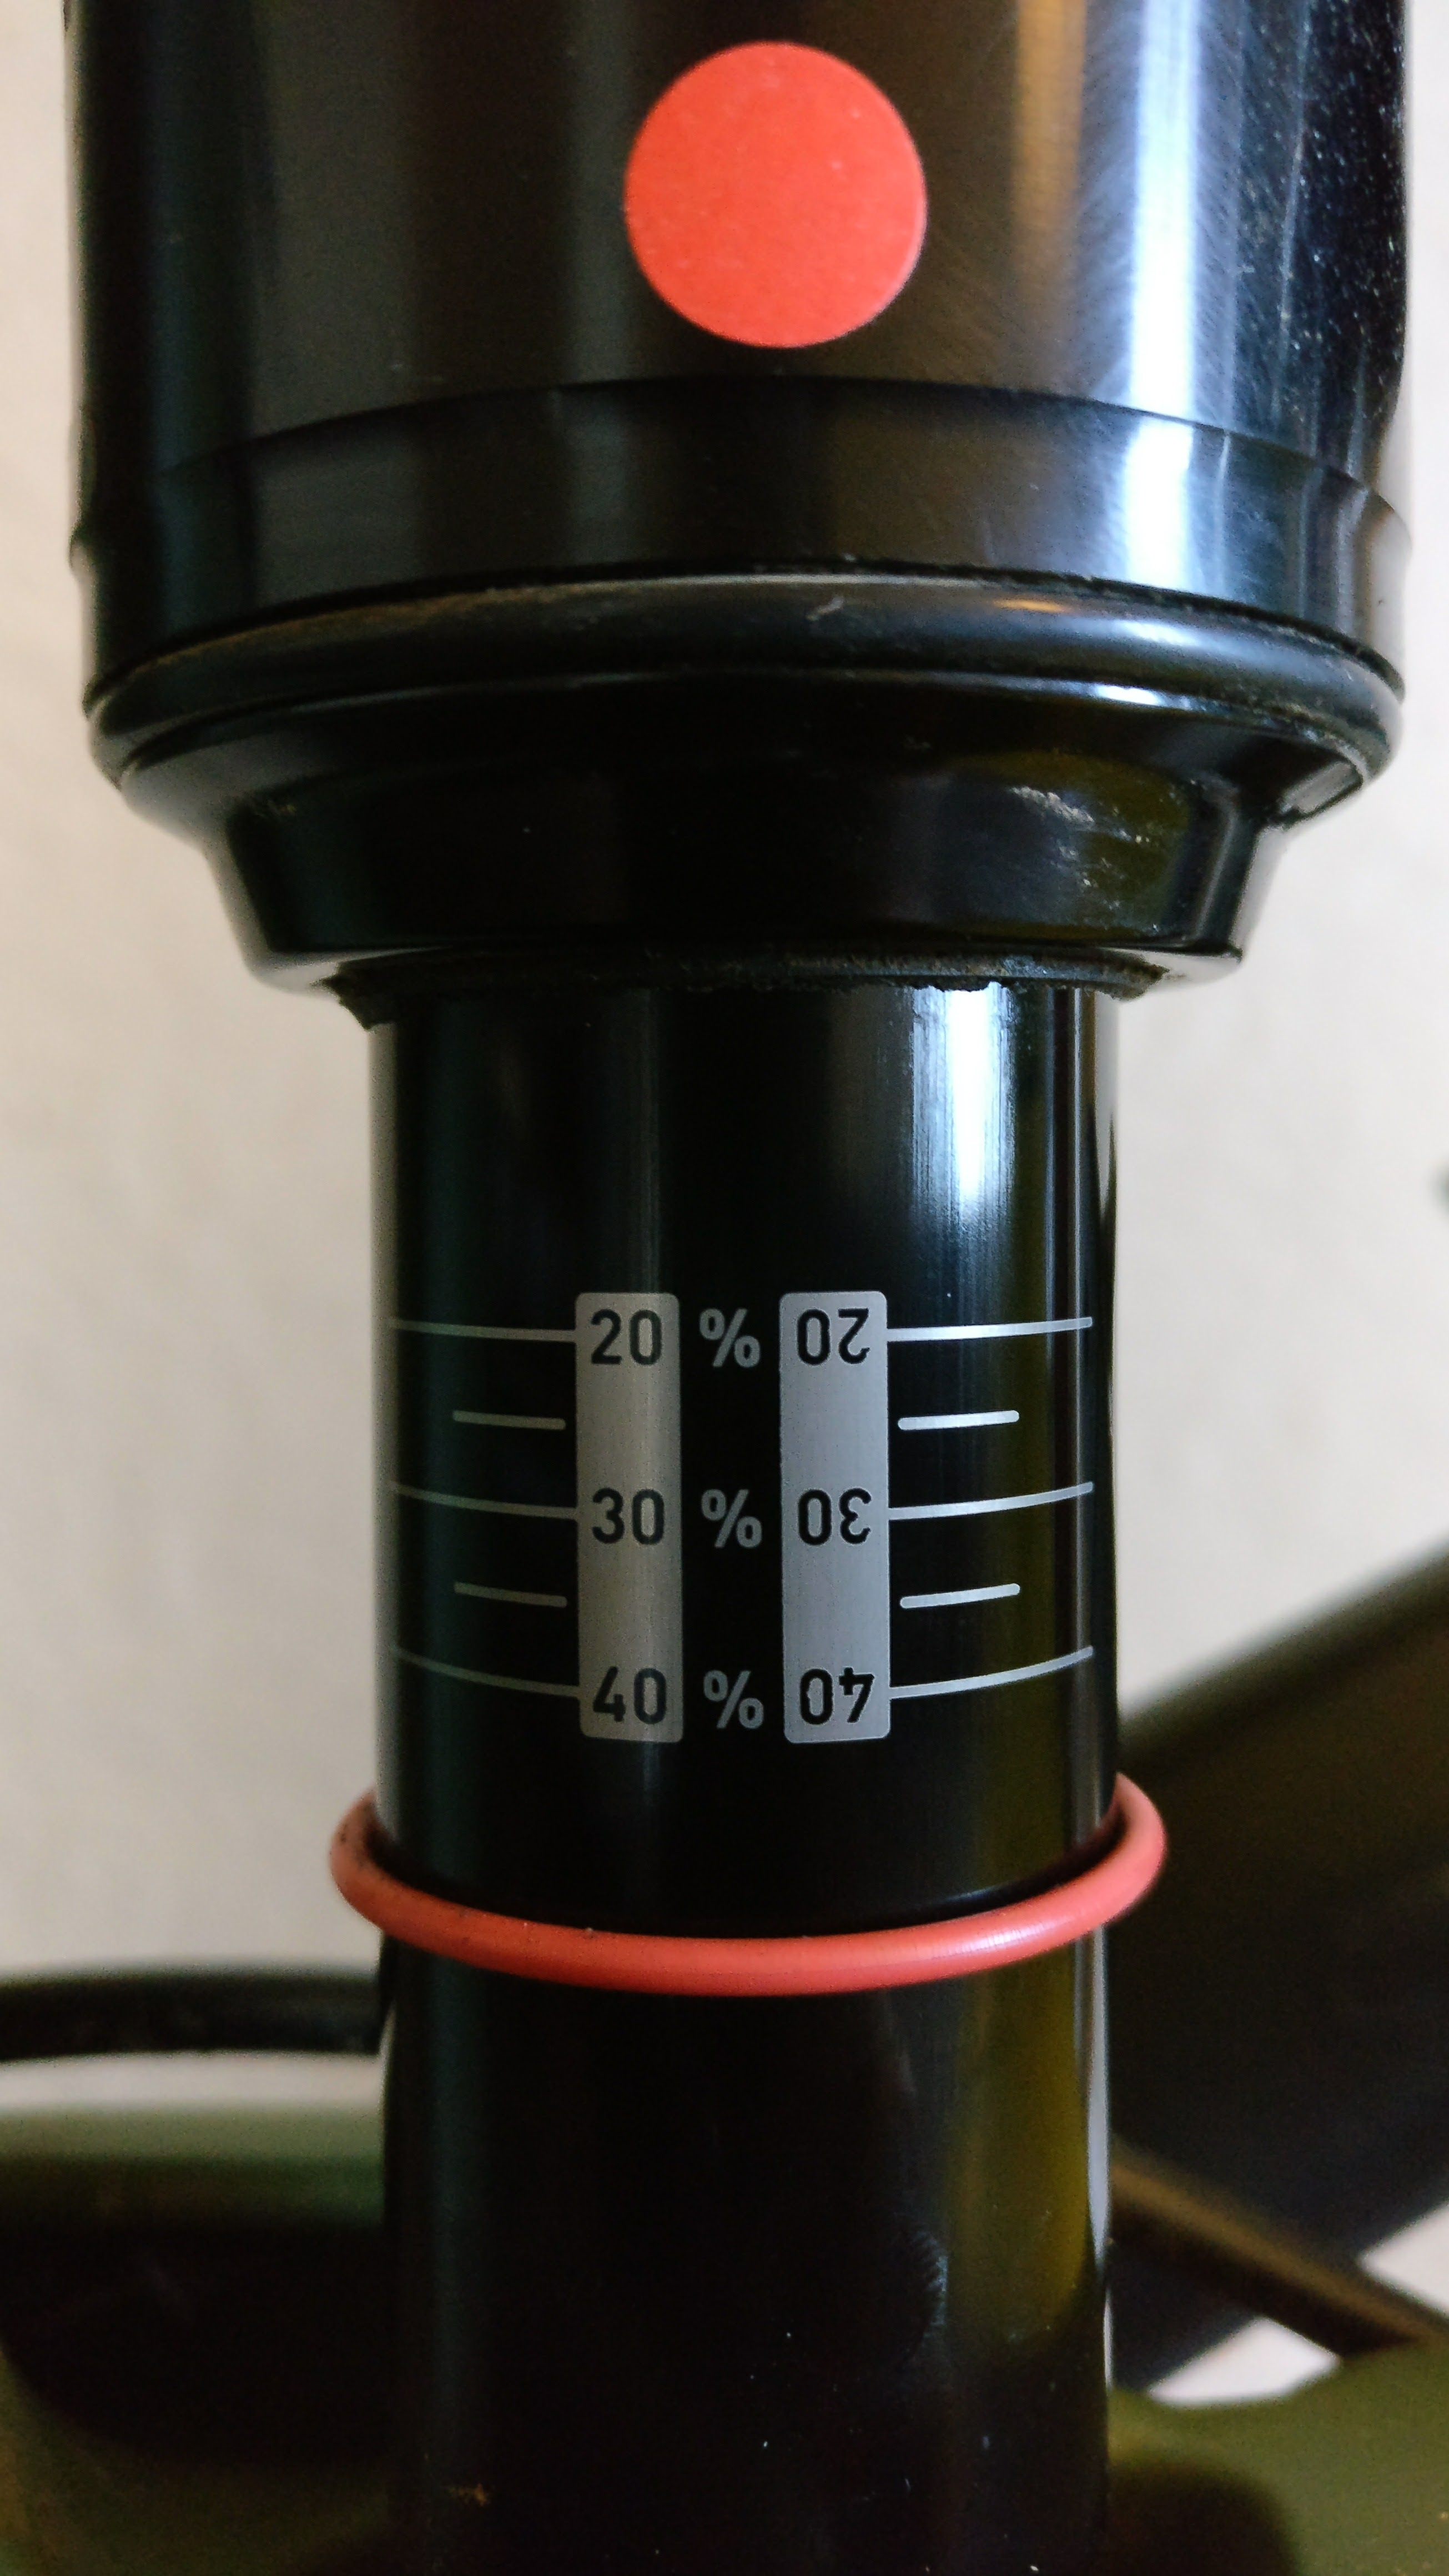
\includegraphics[scale=0.1,trim={0 140cm 0 0}, clip]{../images/results/100_rs.jpg}
				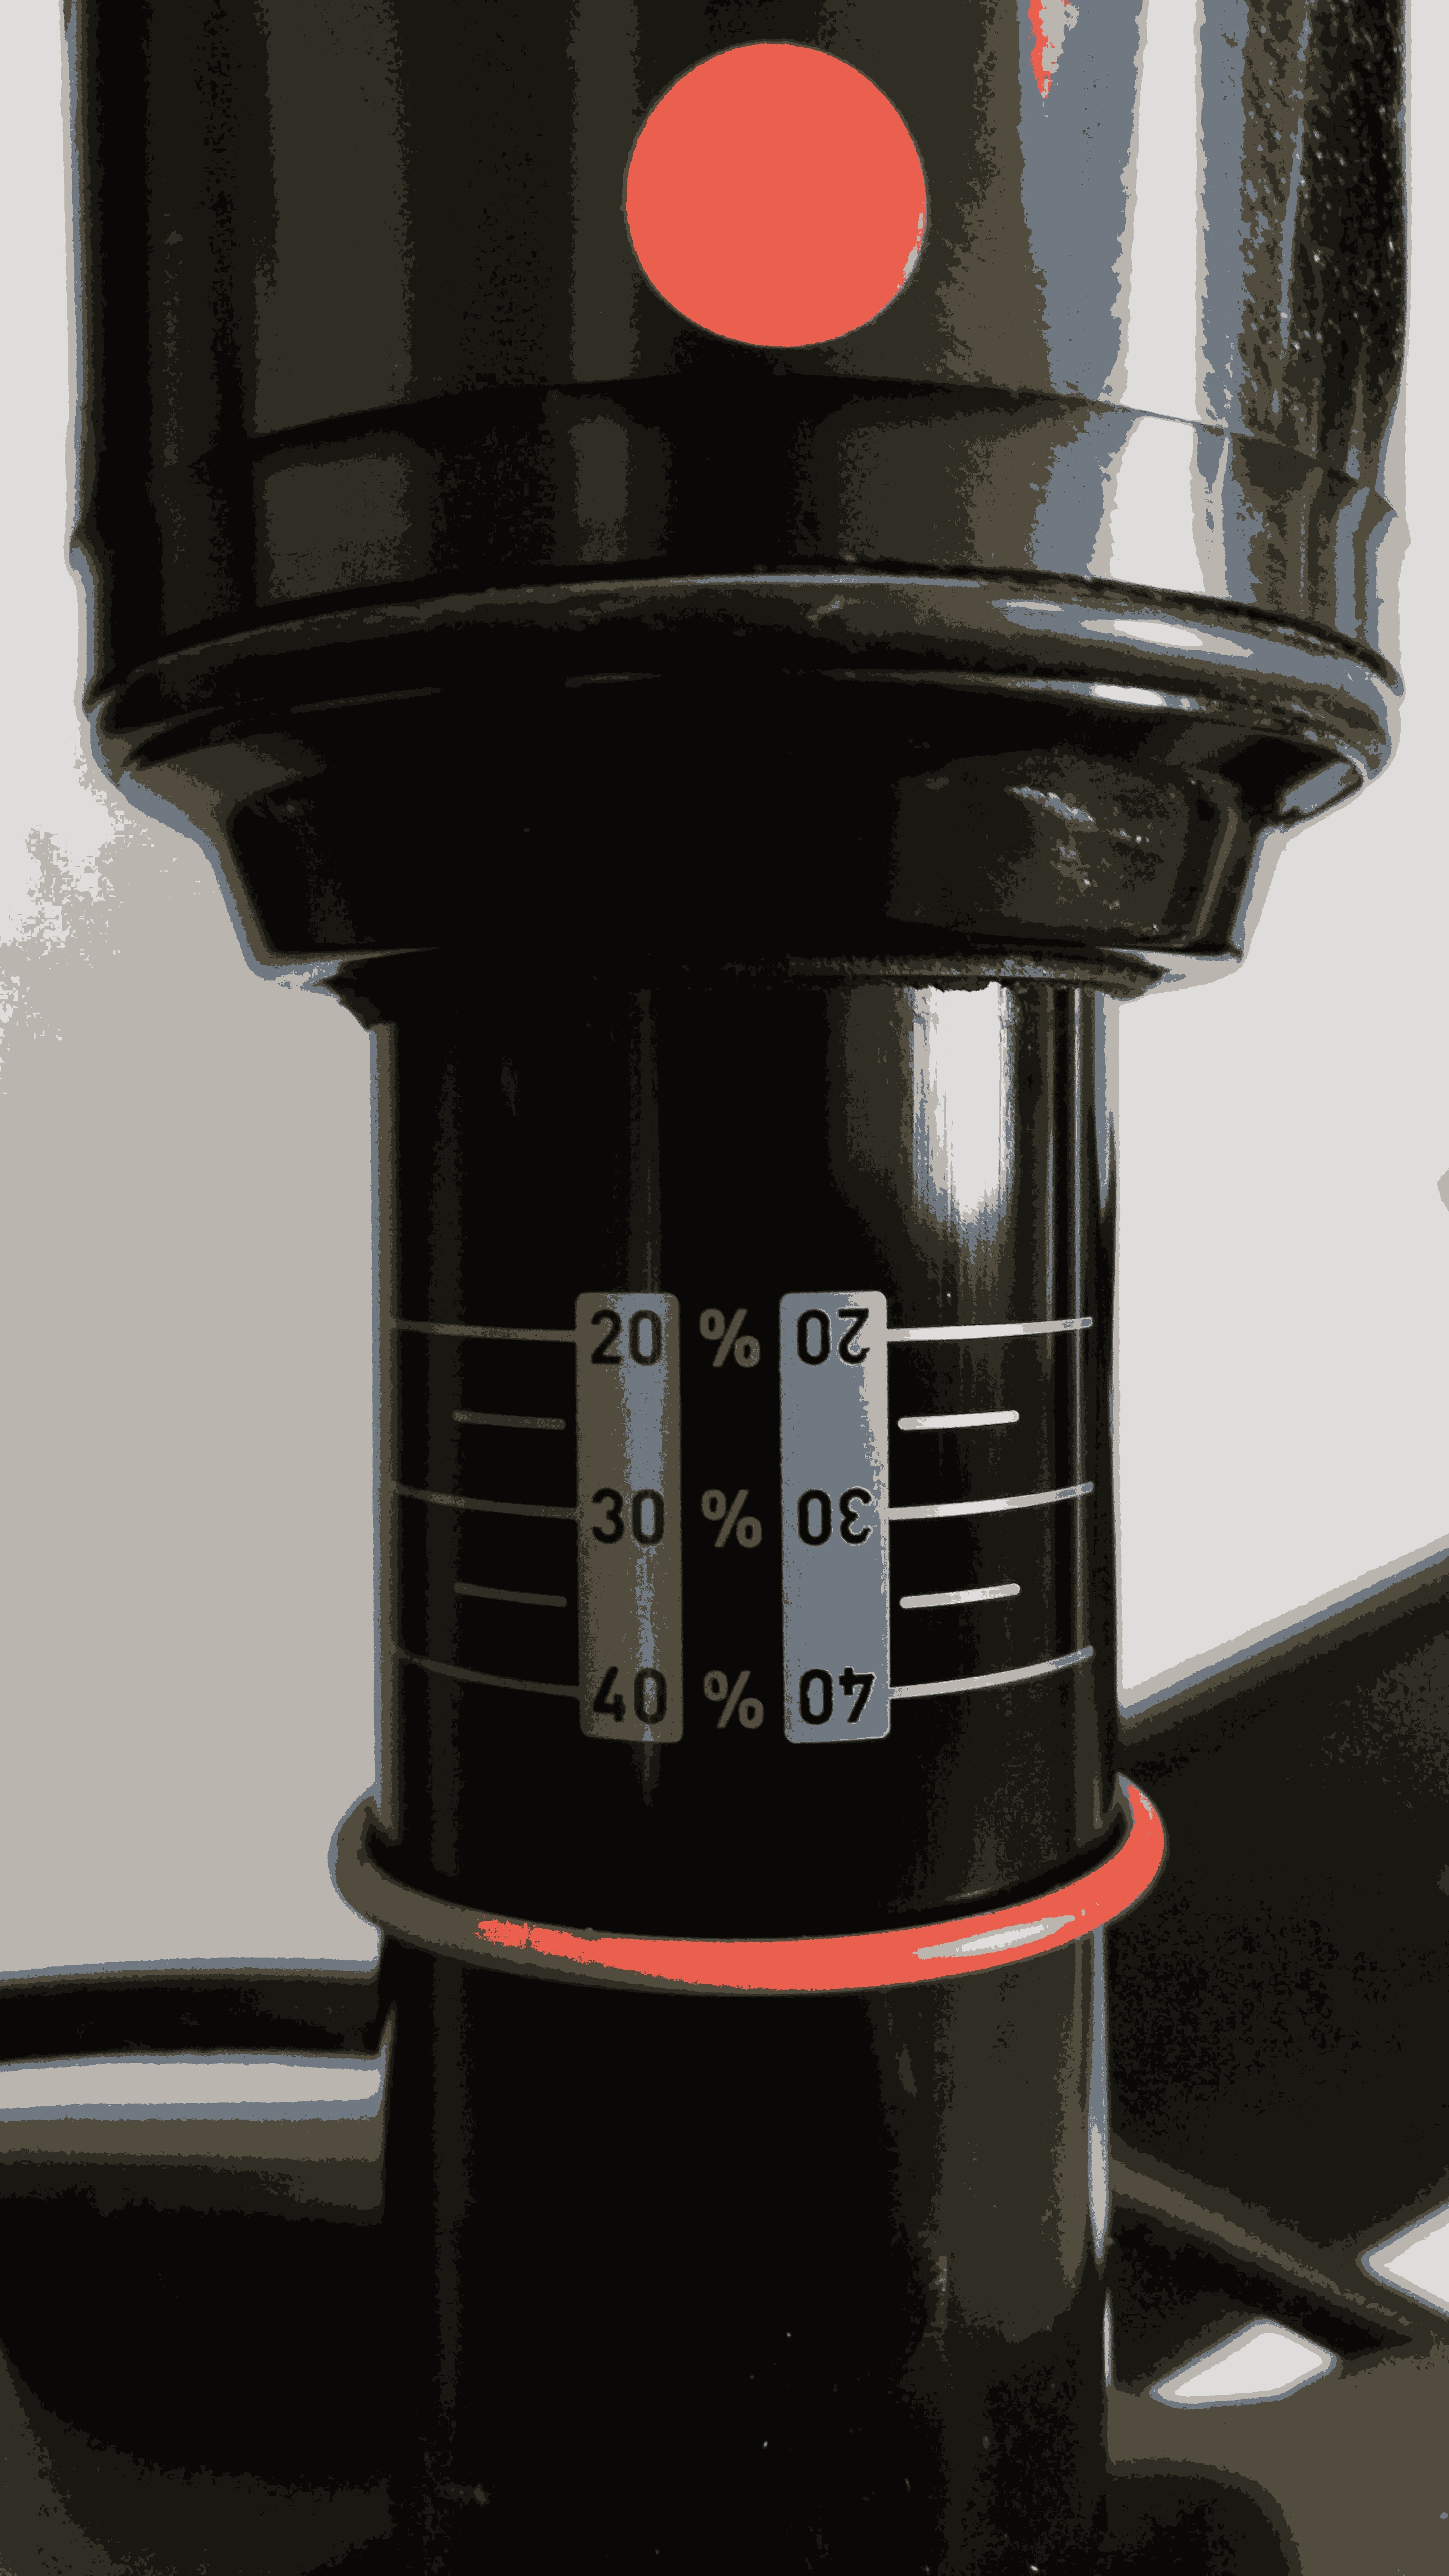
\includegraphics[scale=0.1,trim={0 140cm 0 0},clip]{../images/results/quant.jpg}
				\caption[Normal image versus quantified colours]{Normal image (top) versus quantified colours (bottom)}
				\label{fig:quantified_colours}
			\end{figure}
		\subsubsection{Dynamic Measurement Limits}
			It was decided that the application should utilise the distance between the shock wiper seal and the marker O-ring for providing the sag measurement. This was deemed suitable as the manual process to calculate sag also uses the O-ring which is a prominent feature on most shocks, unless removed by the owner. Initial versions of the application assumed it would find the O-ring somewhere about two thirds of the way up the image height although once multiple images were used from two different makes of shocks this assumption proved to be incorrect.
			\\\\
			To address this and ensure the application is always able to find the O-ring no matter where it appears in the image, it was necessary to use a dynamic method to detect it. In much the same way that using quantified colours solved the issues of detecting the reference point, OpenCV’s {\ttfamily findContours} can be used to find an O-ring of a known colour as long as it is present in the image. When located, a bounding box is drawn around the contour as shown in Figure \ref{fig:find_oring} and this can be used to determine the lowest point at which the O-ring appears in the image to establish the limit of measurement.
			\begin{figure}[h!]
				\centering
				\begin{minipage}{0.4\textwidth}
					\centering
					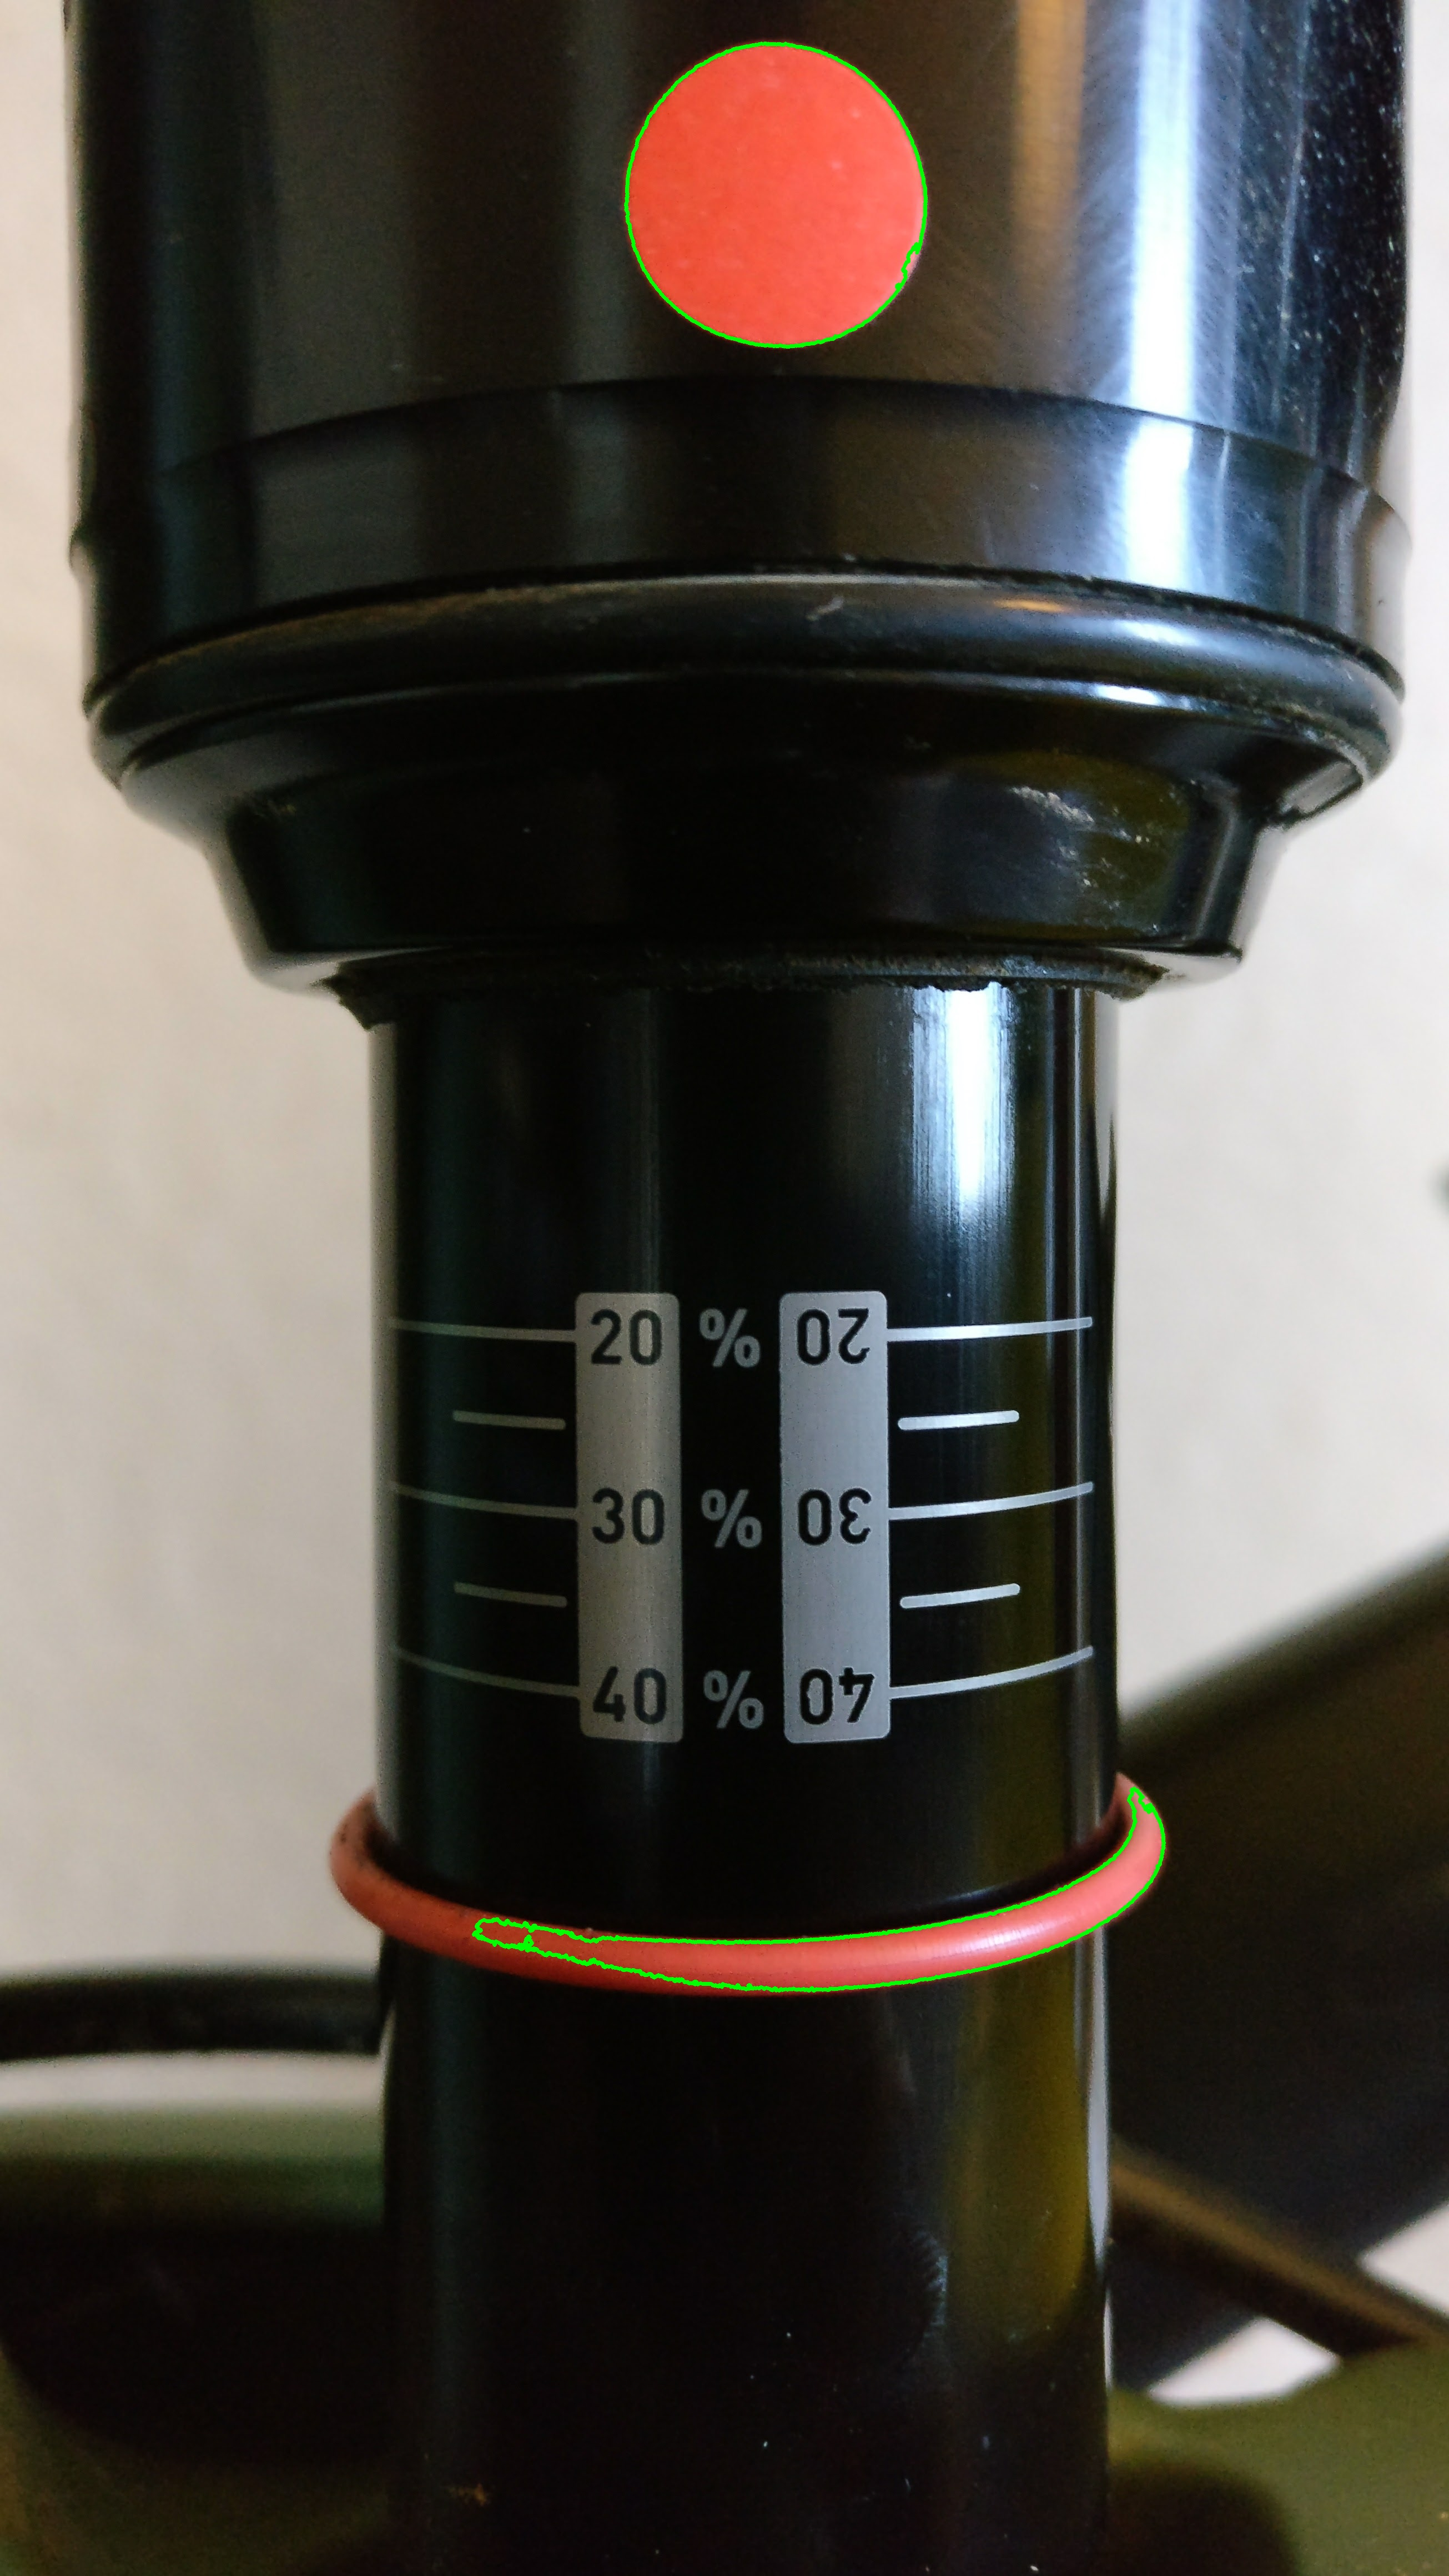
\includegraphics[scale=0.1,
					trim={20cm 30cm 15cm 110cm},
					clip]{../images/results/contours.jpg}				
				\end{minipage}
				\begin{minipage}{0.4\textwidth}
					\centering
					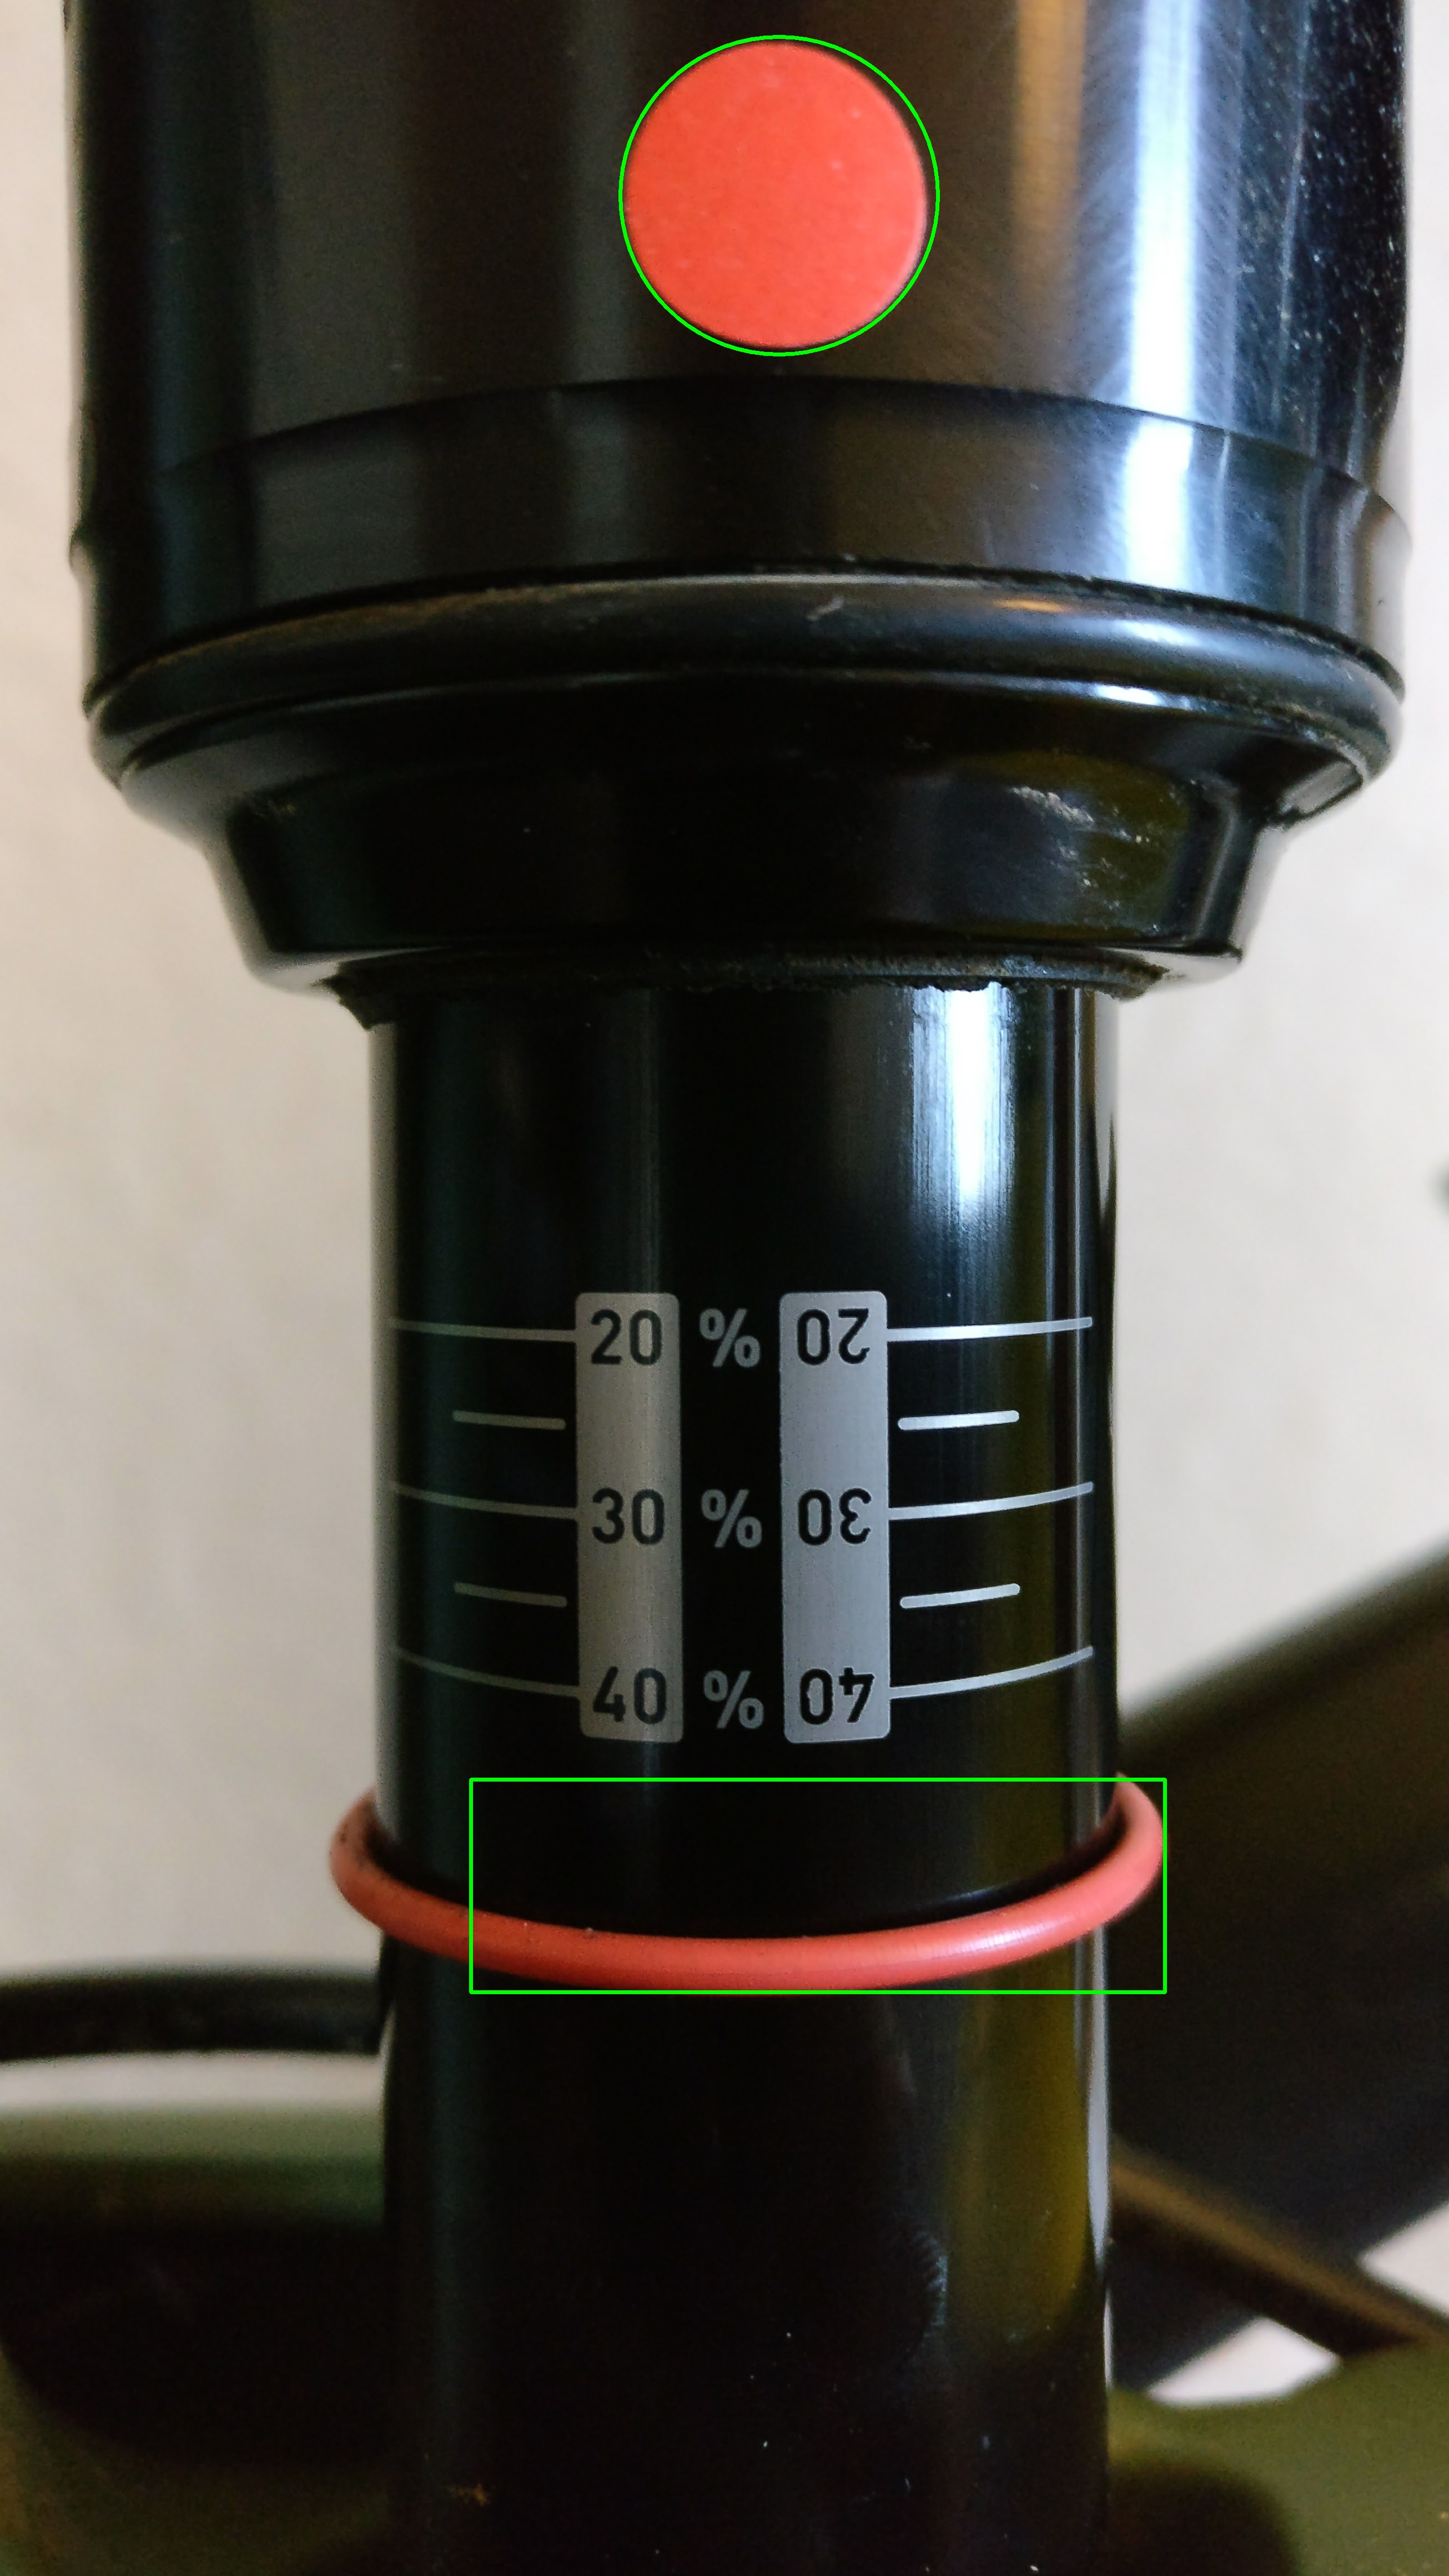
\includegraphics[scale=0.1,
					trim={20cm 30cm 15cm 110cm},
					clip]{../images/results/raw_refs.jpg}				
				\end{minipage}\hfill
				\caption[Red O-ring found using {\ttfamily findContours} with {\ttfamily boundingBox} applied]{Red O-ring found using {\ttfamily findContours} (left) with {\ttfamily boundingBox} applied (right)}
				\label{fig:find_oring}
			\end{figure}
			\\
			As some shocks do not have a coloured O-ring, this process was adapted to locate a black O-ring. This was not successful as black is much less prominent and an alternative method was used. Thresholding is applied to the image and contours produced from the reflections on the telescopic shaft of the shock unit. This made it easy for the application to detect the discontinuity between the O-ring and the shaft so the same bounding box could be applied and used to establish the lower limit for where the application can measure. This result is shown in Figure \ref{fig:black_oring}.
			\begin{figure}[h!]
				\centering
				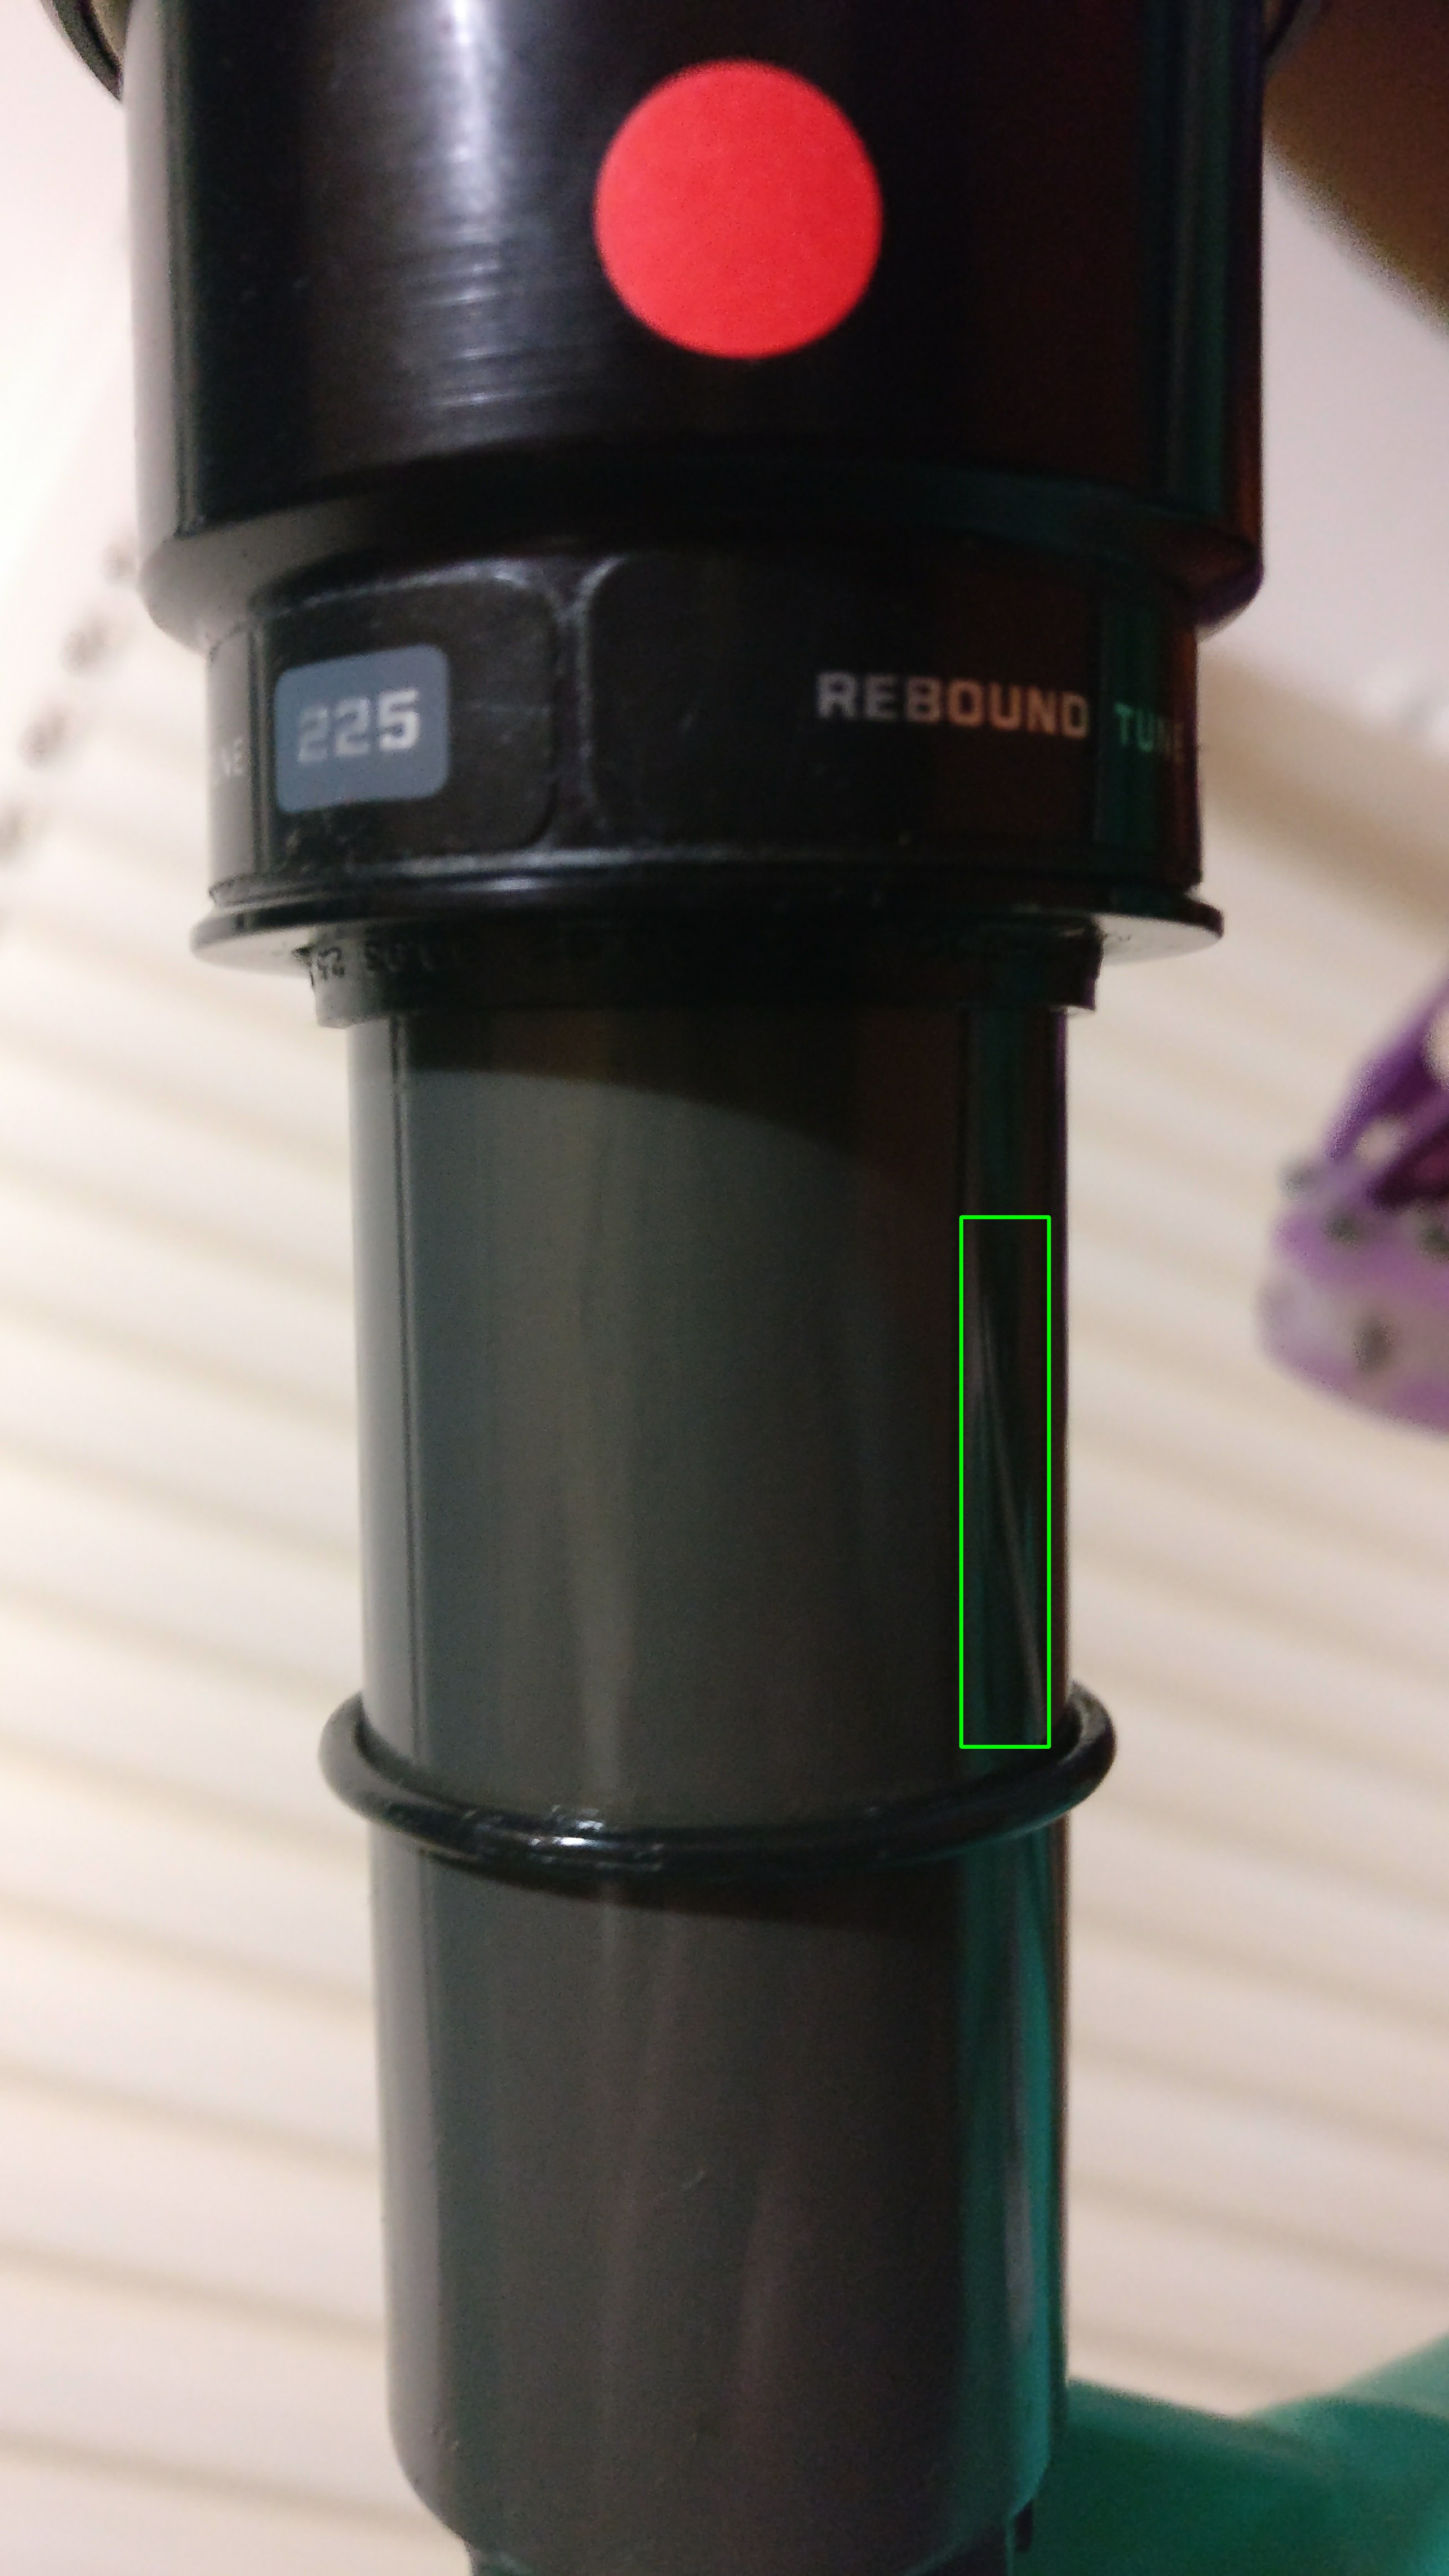
\includegraphics[scale=0.1,trim={20cm 40cm 20cm 70cm},clip]{../images/results/fox_oring.jpg}
				\caption{Black O-ring found using thresholding and {\ttfamily findContours}}
				\label{fig:black_oring}
			\end{figure}
		\subsubsection{Reference Point Measurement Method}
			To measure the dimensions of the circular reference point, the first process applied was Hough Circle Transform as described in \ref{sec:lit_review_hough}. This method was chosen as it is designed specifically to find circles within an image and is simple to implement. Although this did produce measurements, once these values were compared with values derived by manually measuring the image, they proved to be unreliable with variances both above and below the actual value. This effect is shown in Figure \ref{fig:hough_circle} where it is clear that the circle identified using Hough Circle Transform is much smaller than the actual reference point.
			\begin{figure}[h!]
				\centering
				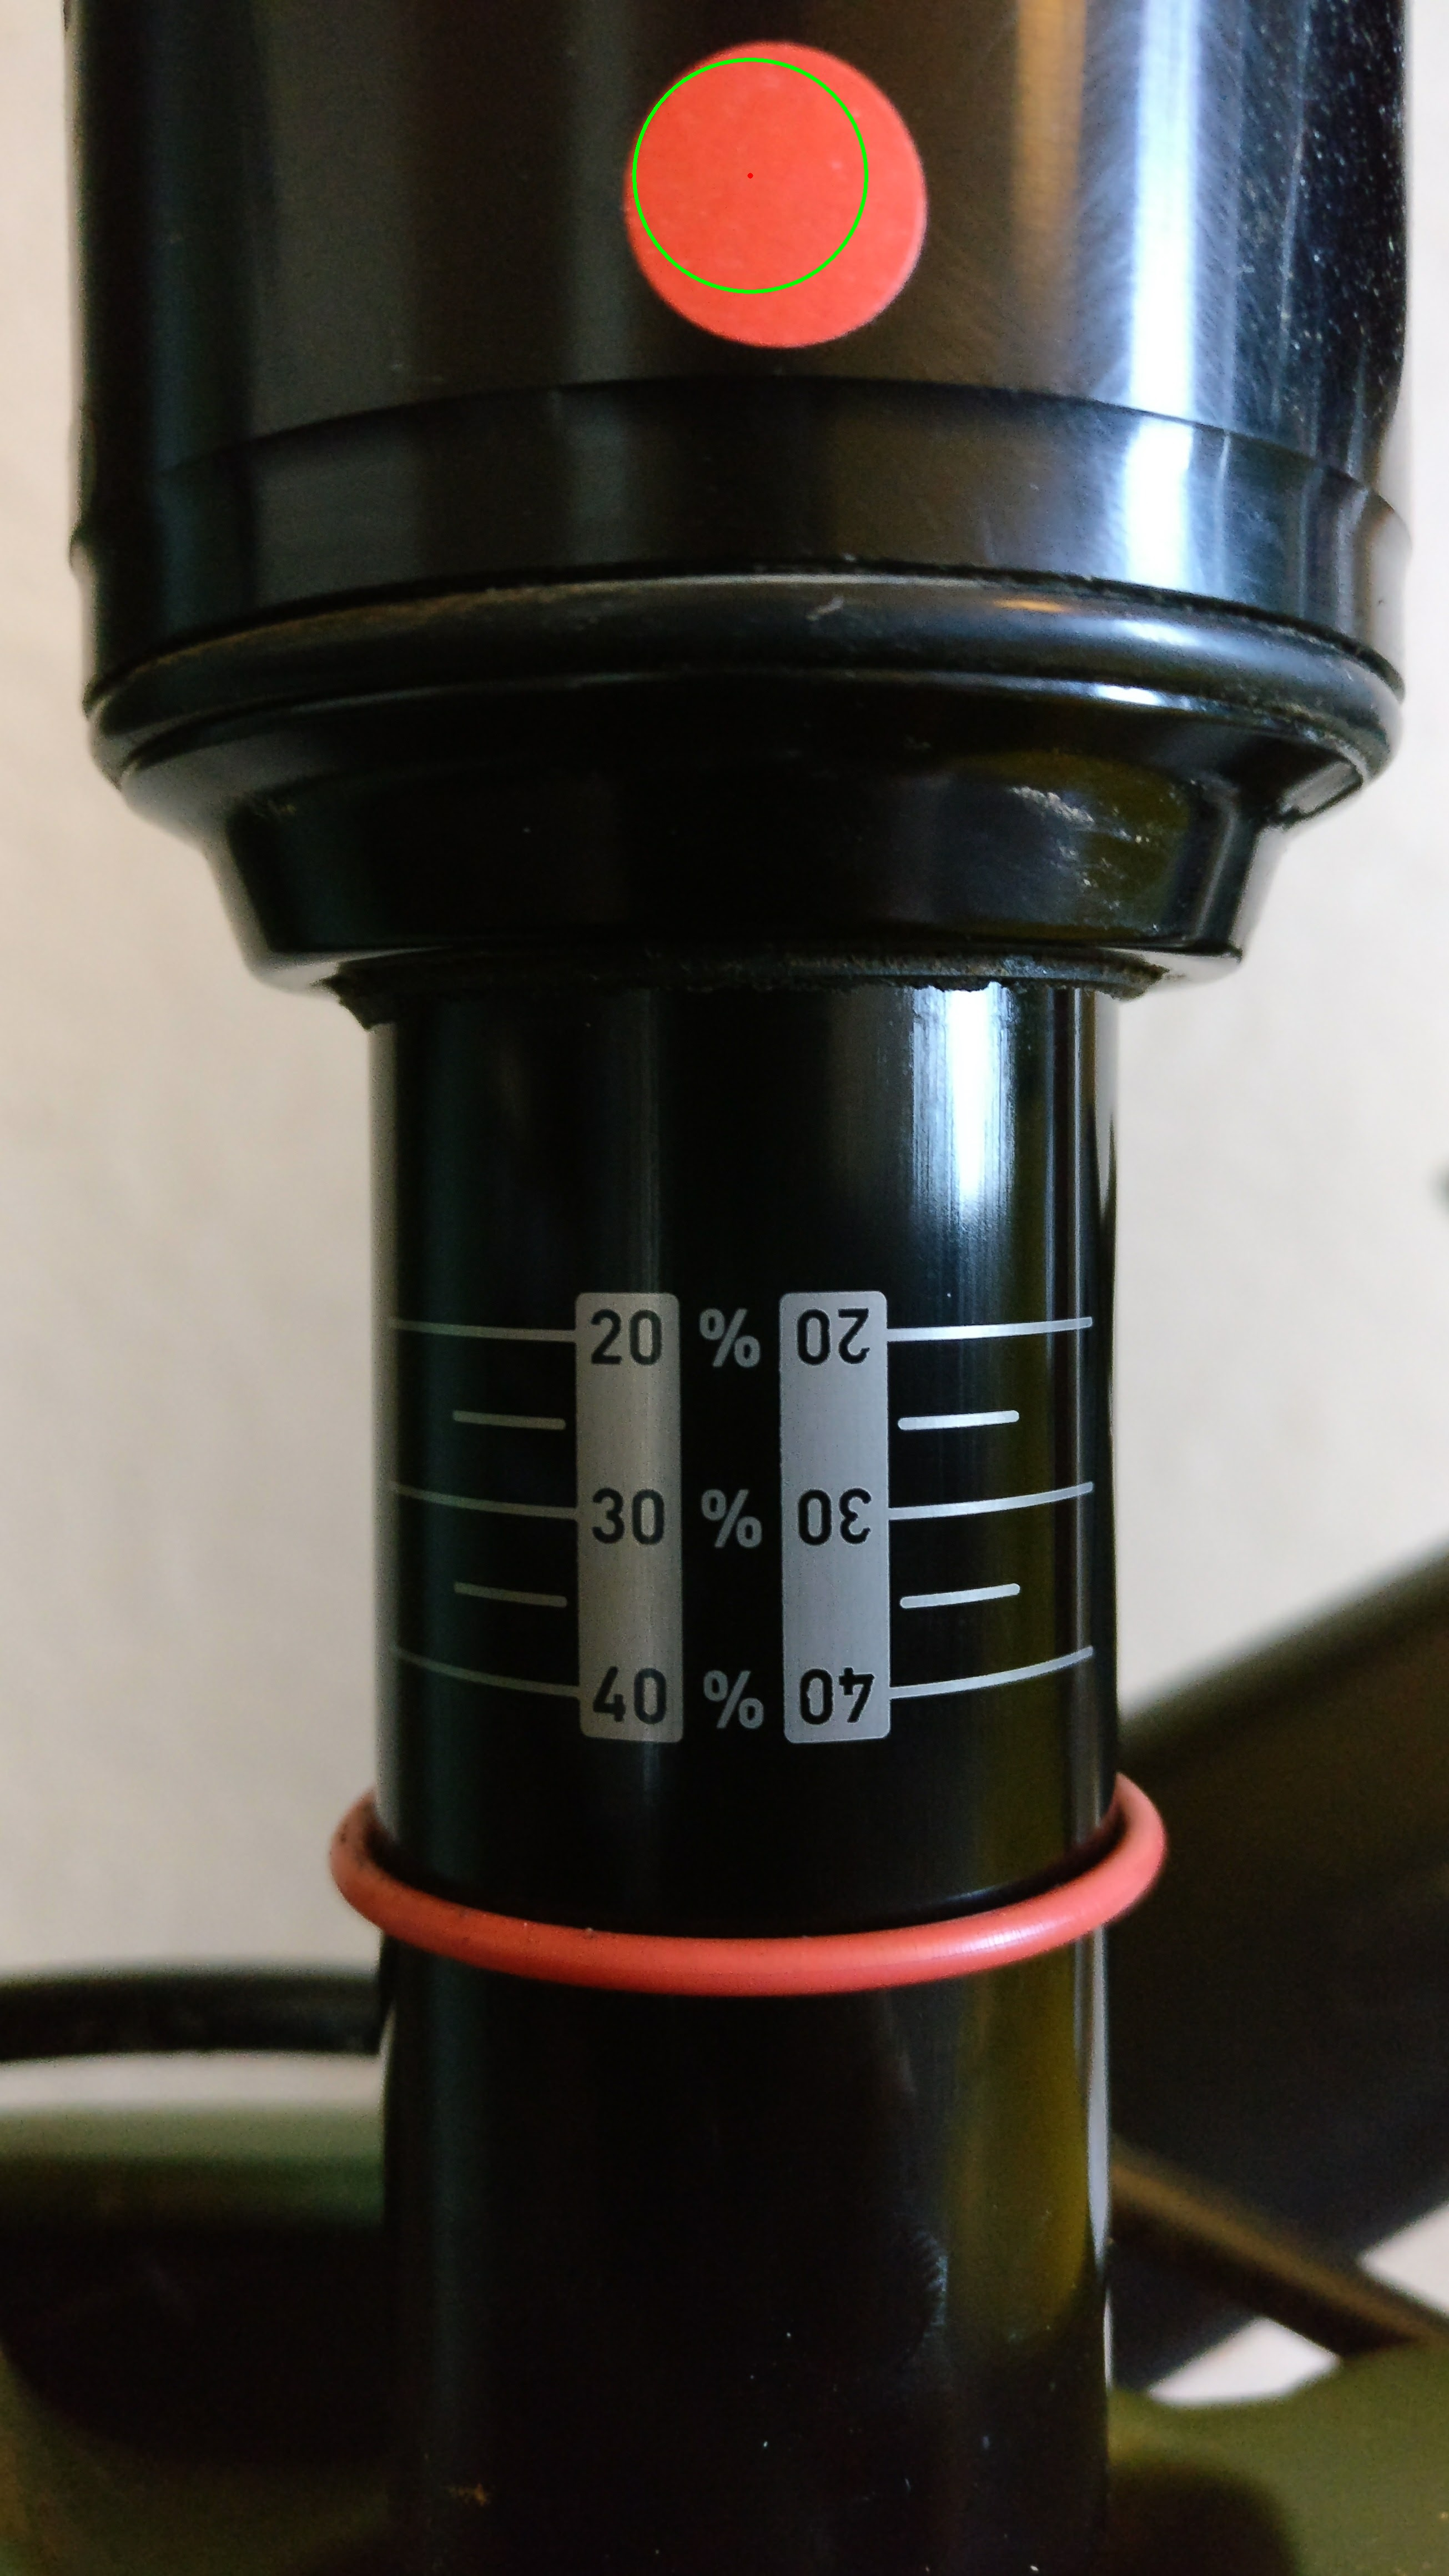
\includegraphics[scale=0.1,
				trim={30cm 140cm 25cm 0},
				clip]{../images/results/HoughCircles.jpg}
				\caption{Reference point found using Hough Circle Transform}
				\label{fig:hough_circle}
			\end{figure}
			\\\\
			To overcome this issue it was necessary to again use OpenCV’s {\ttfamily findContours} in exactly the same way it used to successfully locate the O-ring. Once a contour is found that encompasses the entire reference point, a bounding circle can be drawn around it as shown in Figure \ref{fig:find_ref}. Although the bounding circle appears to be slightly larger than the reference point, experimentation with a variety of images showed that this method produced measurements that were within acceptable tolerances for the pixel per millimetre calculation.
			\\\\
			The reason the Hough Circle method produced a bounding circle that is slightly different to the reference point is because the reference point captured in the image is not a uniform circle. Although the thresholds of the Hough Circle method can be adjusted, applying the sticker to the cylindrical body of the shock unit means it is too misshapen to be detected correctly without the use of OpenCV’s {\ttfamily findContours}.
			\begin{figure}[h!]
				\centering
				\begin{minipage}{0.4\textwidth}
					\centering
					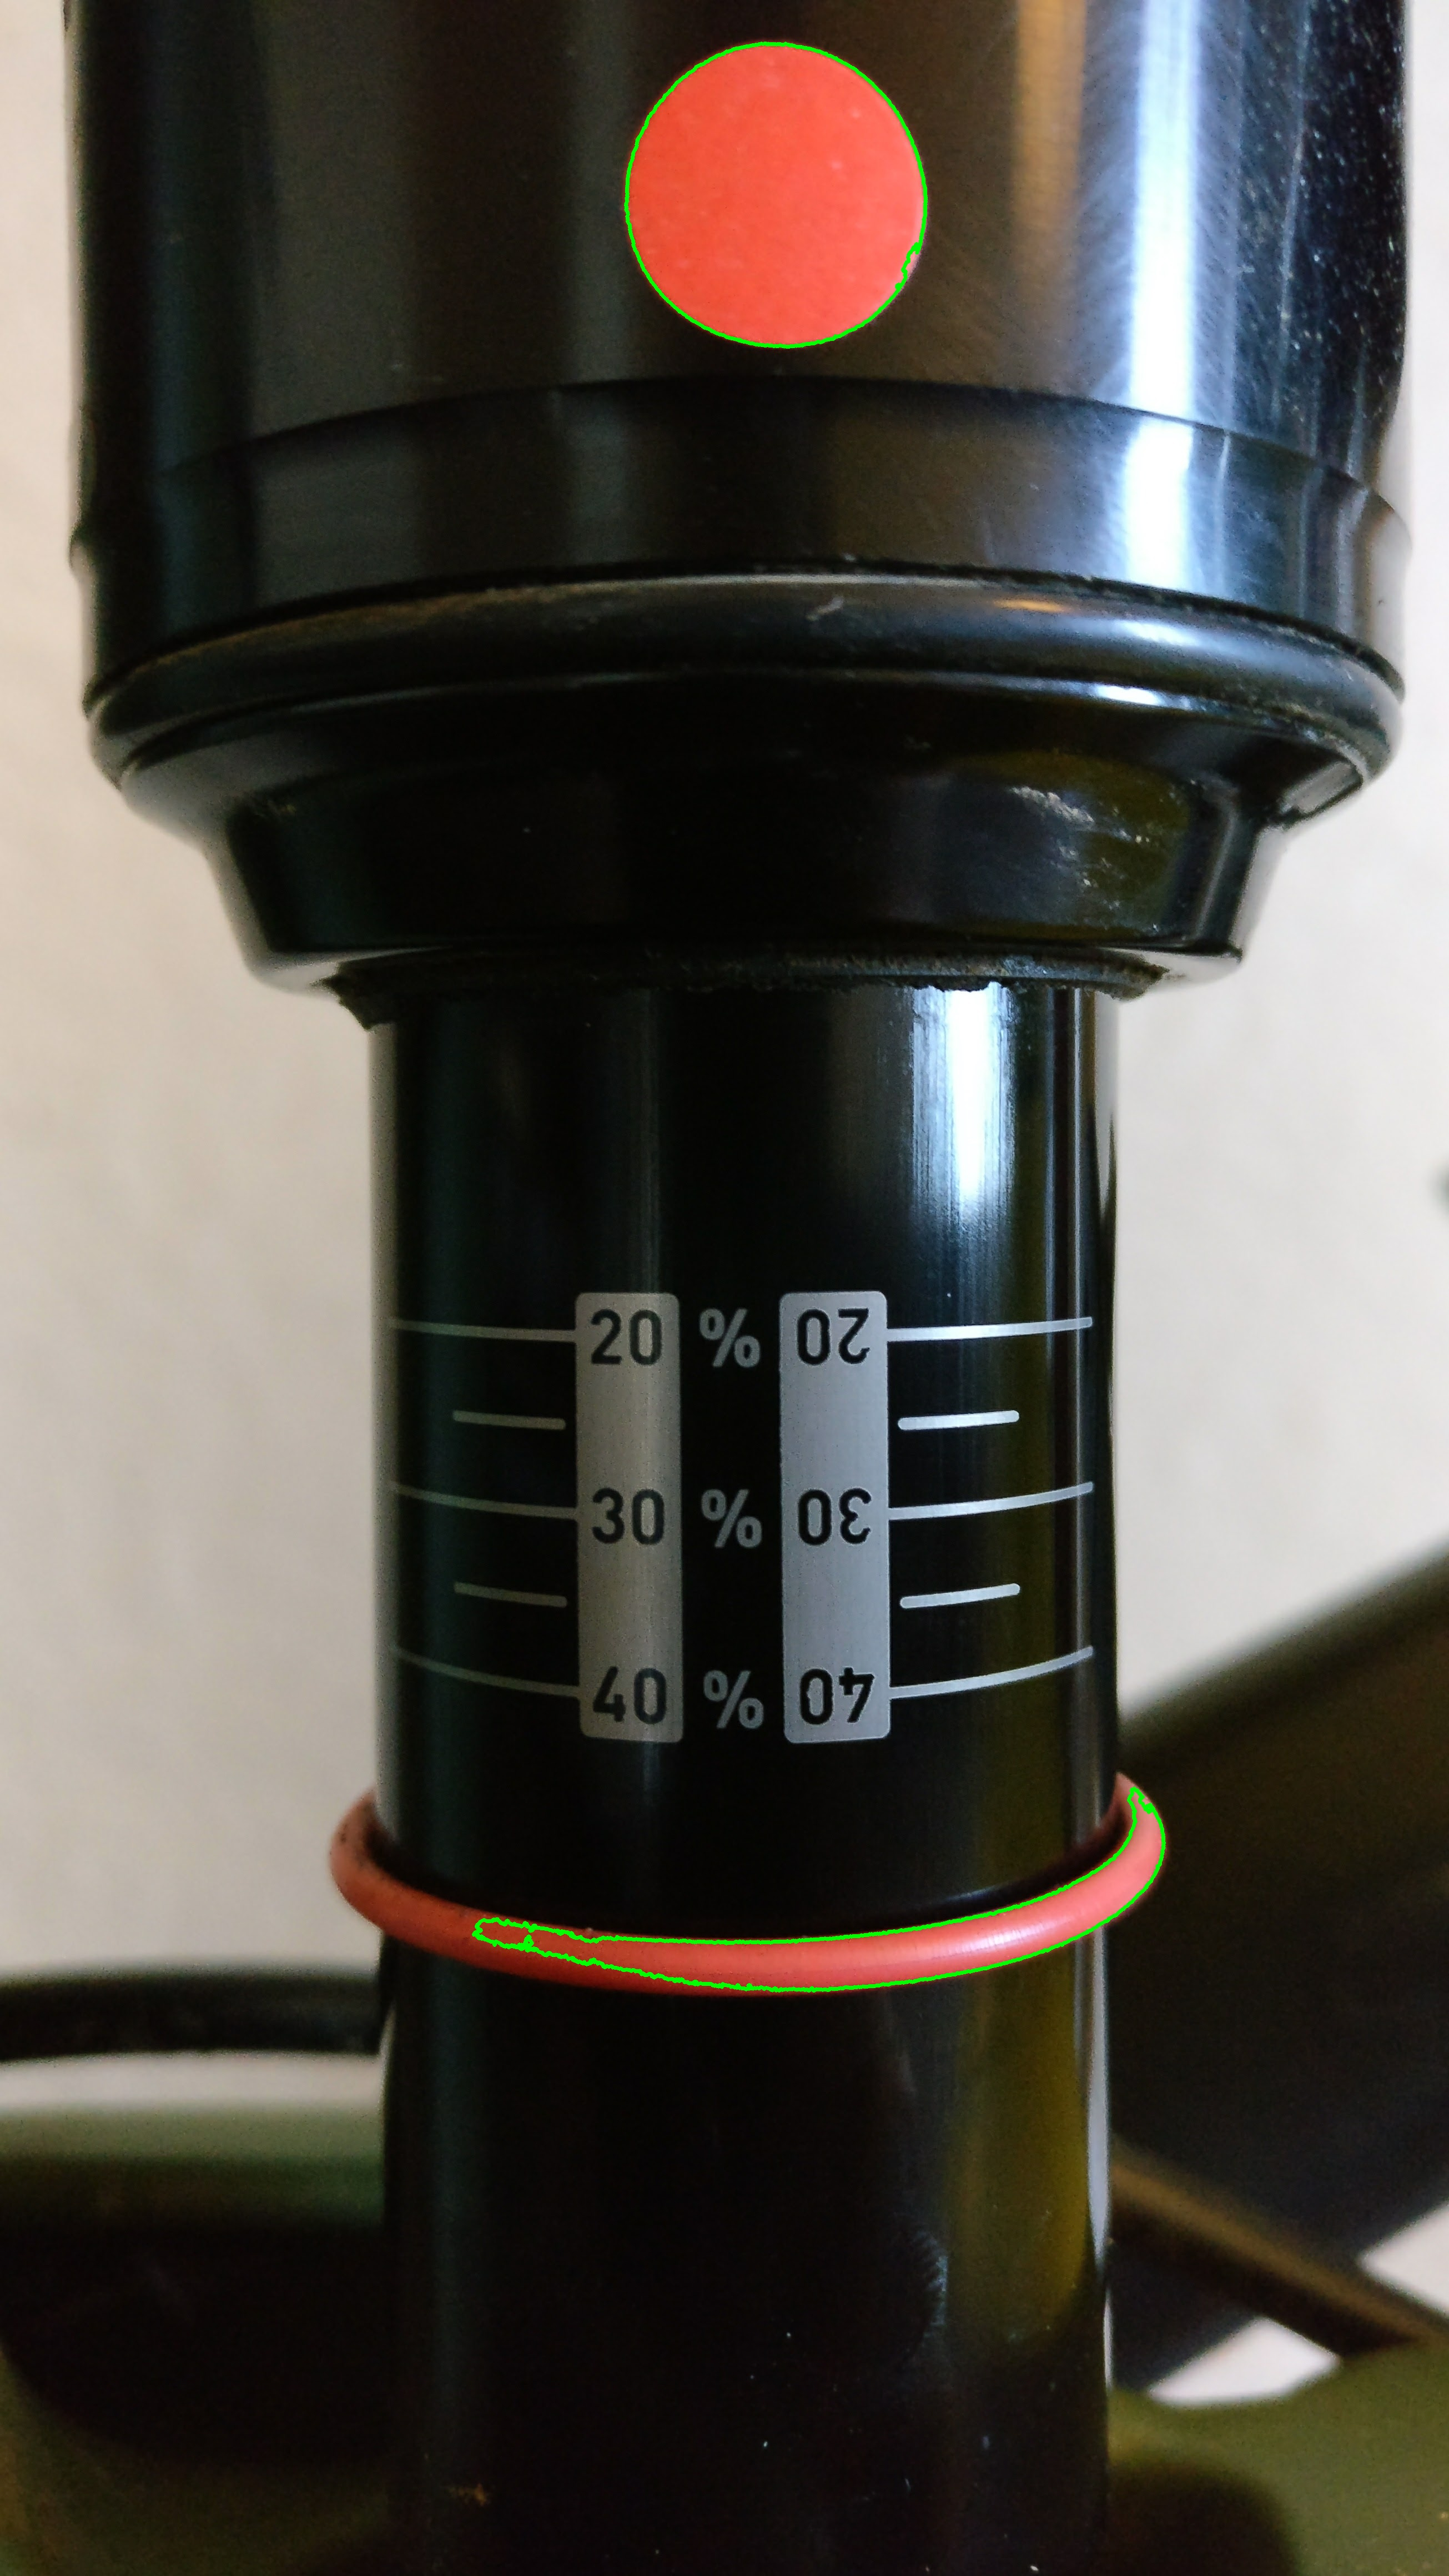
\includegraphics[scale=0.1,
					trim={30cm 140cm 25cm 0},
					clip]{../images/results/contours.jpg}				
				\end{minipage}
				\begin{minipage}{0.4\textwidth}
					\centering
					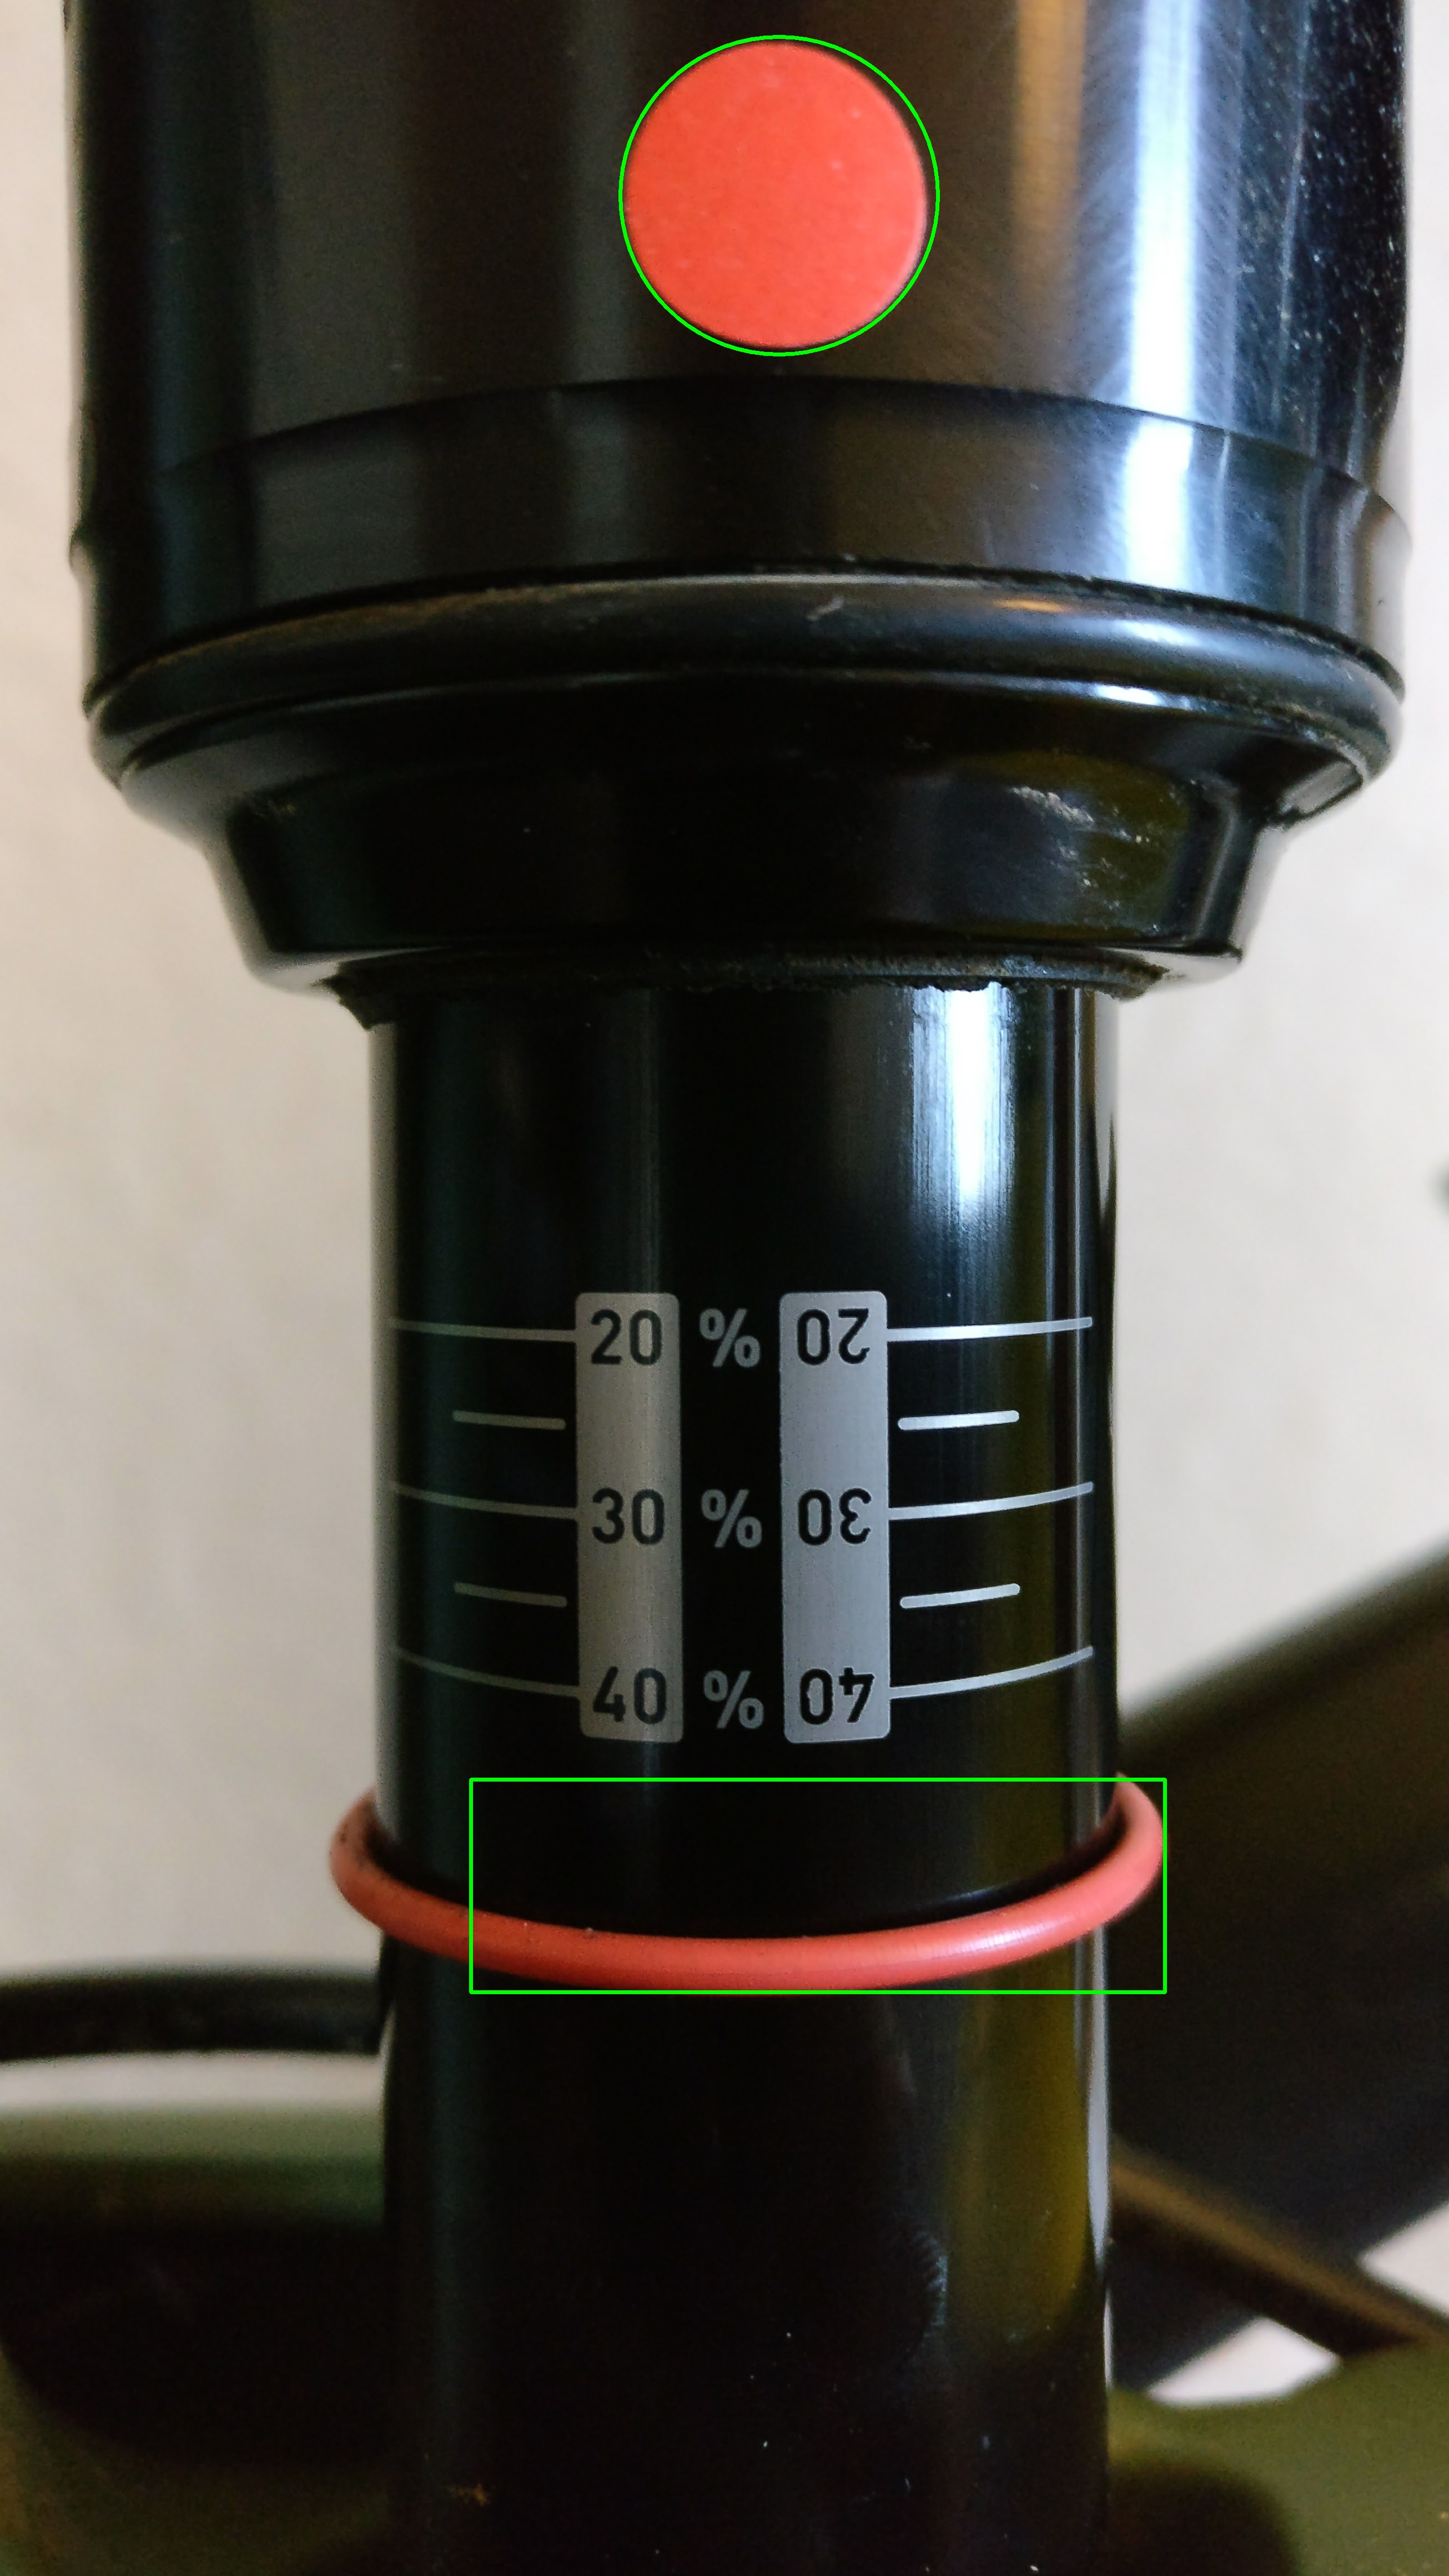
\includegraphics[scale=0.1,
					trim={30cm 140cm 25cm 0},
					clip]{../images/results/raw_refs.jpg}				
				\end{minipage}\hfill
				\caption[Reference point found using {\ttfamily findContours} with {\ttfamily boundingCircle} applied]{Reference point found using {\ttfamily findContours} (left) with {\ttfamily boundingCircle} applied (right)}
				\label{fig:find_ref}
			\end{figure}
		\subsubsection{Pressure Calculation}\label{sec:results_pressure_calculation}
			The original method for producing a suggested pressure that would give the optimal amount of sag was to calculate a pressure per millimetre metric in pounds per square inch (PSI) from the measurement of the shock shaft and the current pressure of the shock supplied by the user. The assumption being that for every 1 PSI of pressure added to the shock, this would reduce the movement by a fixed amount proportionate to the original pressure. The equation for this metric is as follows:
			\begin{equation}
				\label{equ:pxpermm}
				P_s = \Bigg(\frac{P_c}{M_c}\Bigg)M_s
			\end{equation}
			\begin{where}
				\item $P_s$ is the pressure to produce the desired sag setting
				\item $P_c$ is the pressure currently in the shock
				\item $M_s$ is the measurement to produce the desired sag setting
				\item $M_c$ is the current measurement of the shock shaft
			\end{where}
			\vspace{5mm}
			Though this hypothesised method had produced reliable results when tested manually, it failed to do so in the application both when different images, reference points, and desired sag values were tested and even when these values were hard-coded. Further investigation and discussion suggested the cause of this problem was the non-linearity of rear suspension, previously discussed in \ref{sec:lit_review_rear_suspension}, and non-linearity of air springs.
			\\\\
			When an air spring is compressed the spring rate increases through its travel as the particles of air become increasingly compressed \citep{goodyear2014air}. While this effect still allows the shock unit to be fine tuned, applying a linear equation to a non-linear phenomenon is clearly going to produce some degree of error. However as the range of measurement in this project is small compared to the full stroke of an air shock, it was theorised that the spring rate can be considered linear within the limited range of compression in question.
			\\\\
			To investigate this, the sag of a shock was measured at pressures between 100 and 250 PSI in increments of 10 PSI. This was carried out for two shocks, one with a normal air can and another with a high volume air can, then the collected data was plotted and compared against a trend line generated by linear regression. The results of this can be seen in Figure \ref{fig:scatters}.
			\begin{figure}[h!]
				\centering
				\begin{minipage}{0.4\textwidth}
					\centering
					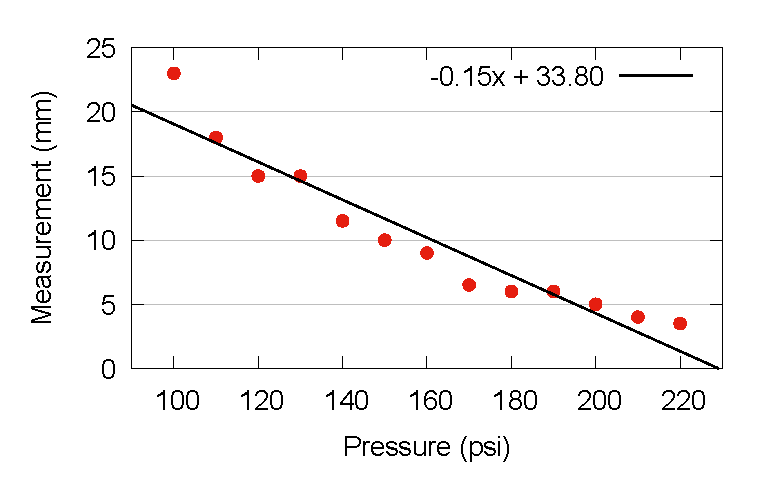
\includegraphics[width=\textwidth]{../images/results/fox_scatter.eps}
				\end{minipage}
				\begin{minipage}{0.4\textwidth}
					\centering
					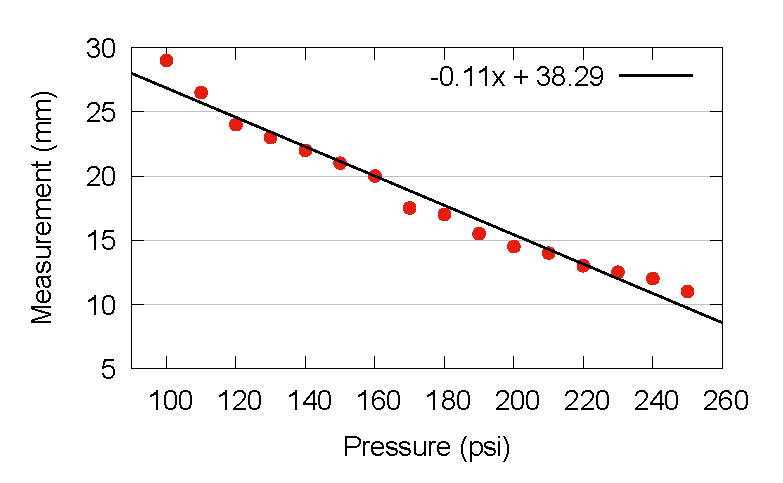
\includegraphics[width=\textwidth]{../images/results/rs_scatter.eps}
				\end{minipage}
				\caption[Sag measurements for standard air shock and high volume air shock]{Sag measurements for standard air shock (left) and high volume air shock (right)}
				\label{fig:scatters}
			\end{figure}\\
			From this data it could be concluded that, within the range of measurements, the compression rate of the air spring is linear. The data-points in Figure \ref{fig:scatters} do occasionally vary though this thought to be due to it being a non-sterile test environment. Both shocks were well-used potentially containing age-related defects and loading the bike was done simply by using body weight.
			\\\\
			Having established that the relationship between the pressure in the shock and movement from weighting the shock could be treated as if it were linear, the plan was to implement an ideal gas equation \citep{burdette2012ideal}. However investigation into producing charts using Python uncovered a method of computationally producing a linear equation. This led to the application’s process being rearranged so that it takes in two images, one of the shock loaded at 100 PSI and another at 150 PSI. Using this data it can produce a virtual plot and linear equation with which to calculate a value for the optimal sag setting.
	\subsection{Application}
		\subsubsection{Images}
			The application requires two images to generate the measurements needed for the calculation. The application can process images in different lighting conditions and ones where a flash has been used though there are some criteria which must be adhered to. There must be a red, circular, 7.5mm diameter sticker on the shock, preferably sited just above the shock seal. The image should also be taken so that the shock seal is around 1/3 down in the image. Examples of the images used are shown in Figure \ref{fig:application_images}.
			\\\\
			The user must supply one image of the shock which has been pressurised to 100 PSI and a second with the shock pressurised to 150 PSI both loaded under the normal riding weight, i.e. complete with helmet, body armour and hydration pack. Each time the marker O-ring should be returned to the top of the shock shaft before weight is applied to the shock.
			\begin{figure}[h!]
				\begin{subfigure}[t]{0.5\textwidth}
					\centering
					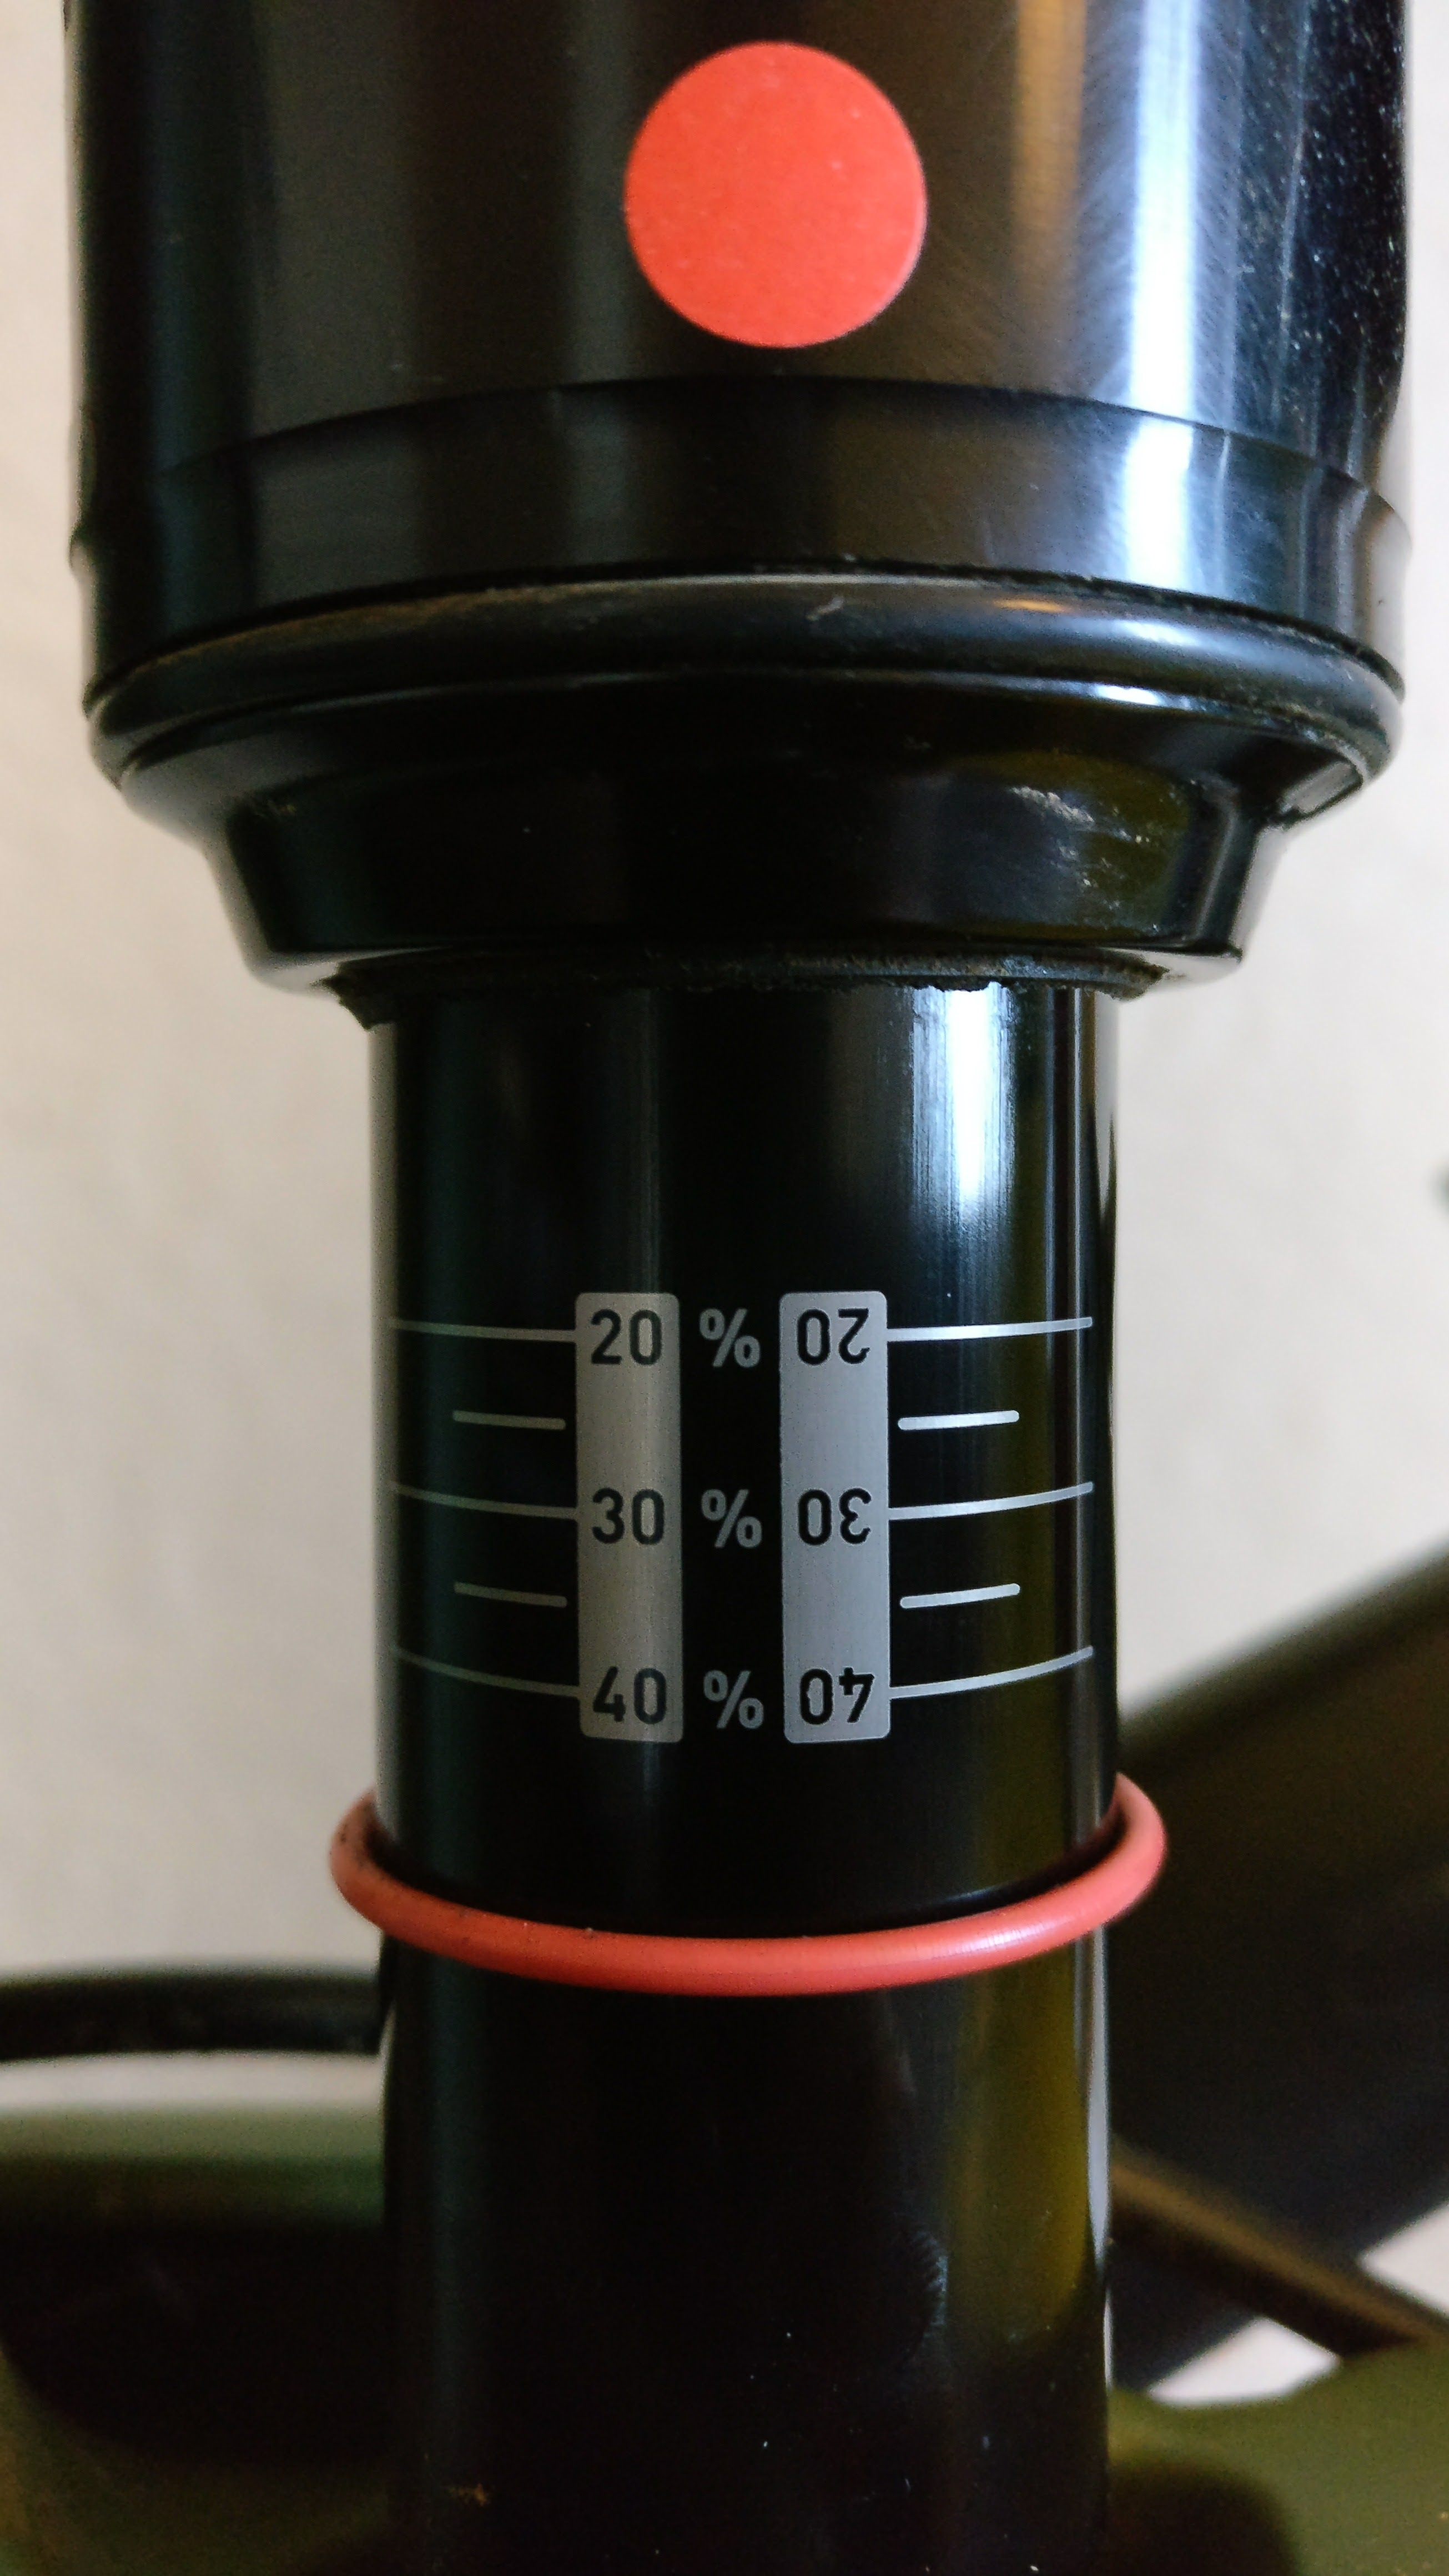
\includegraphics[scale=0.04]{../images/results/100_rs.jpg}
				\end{subfigure}
				\begin{subfigure}[t]{0.5\textwidth}
					\centering
					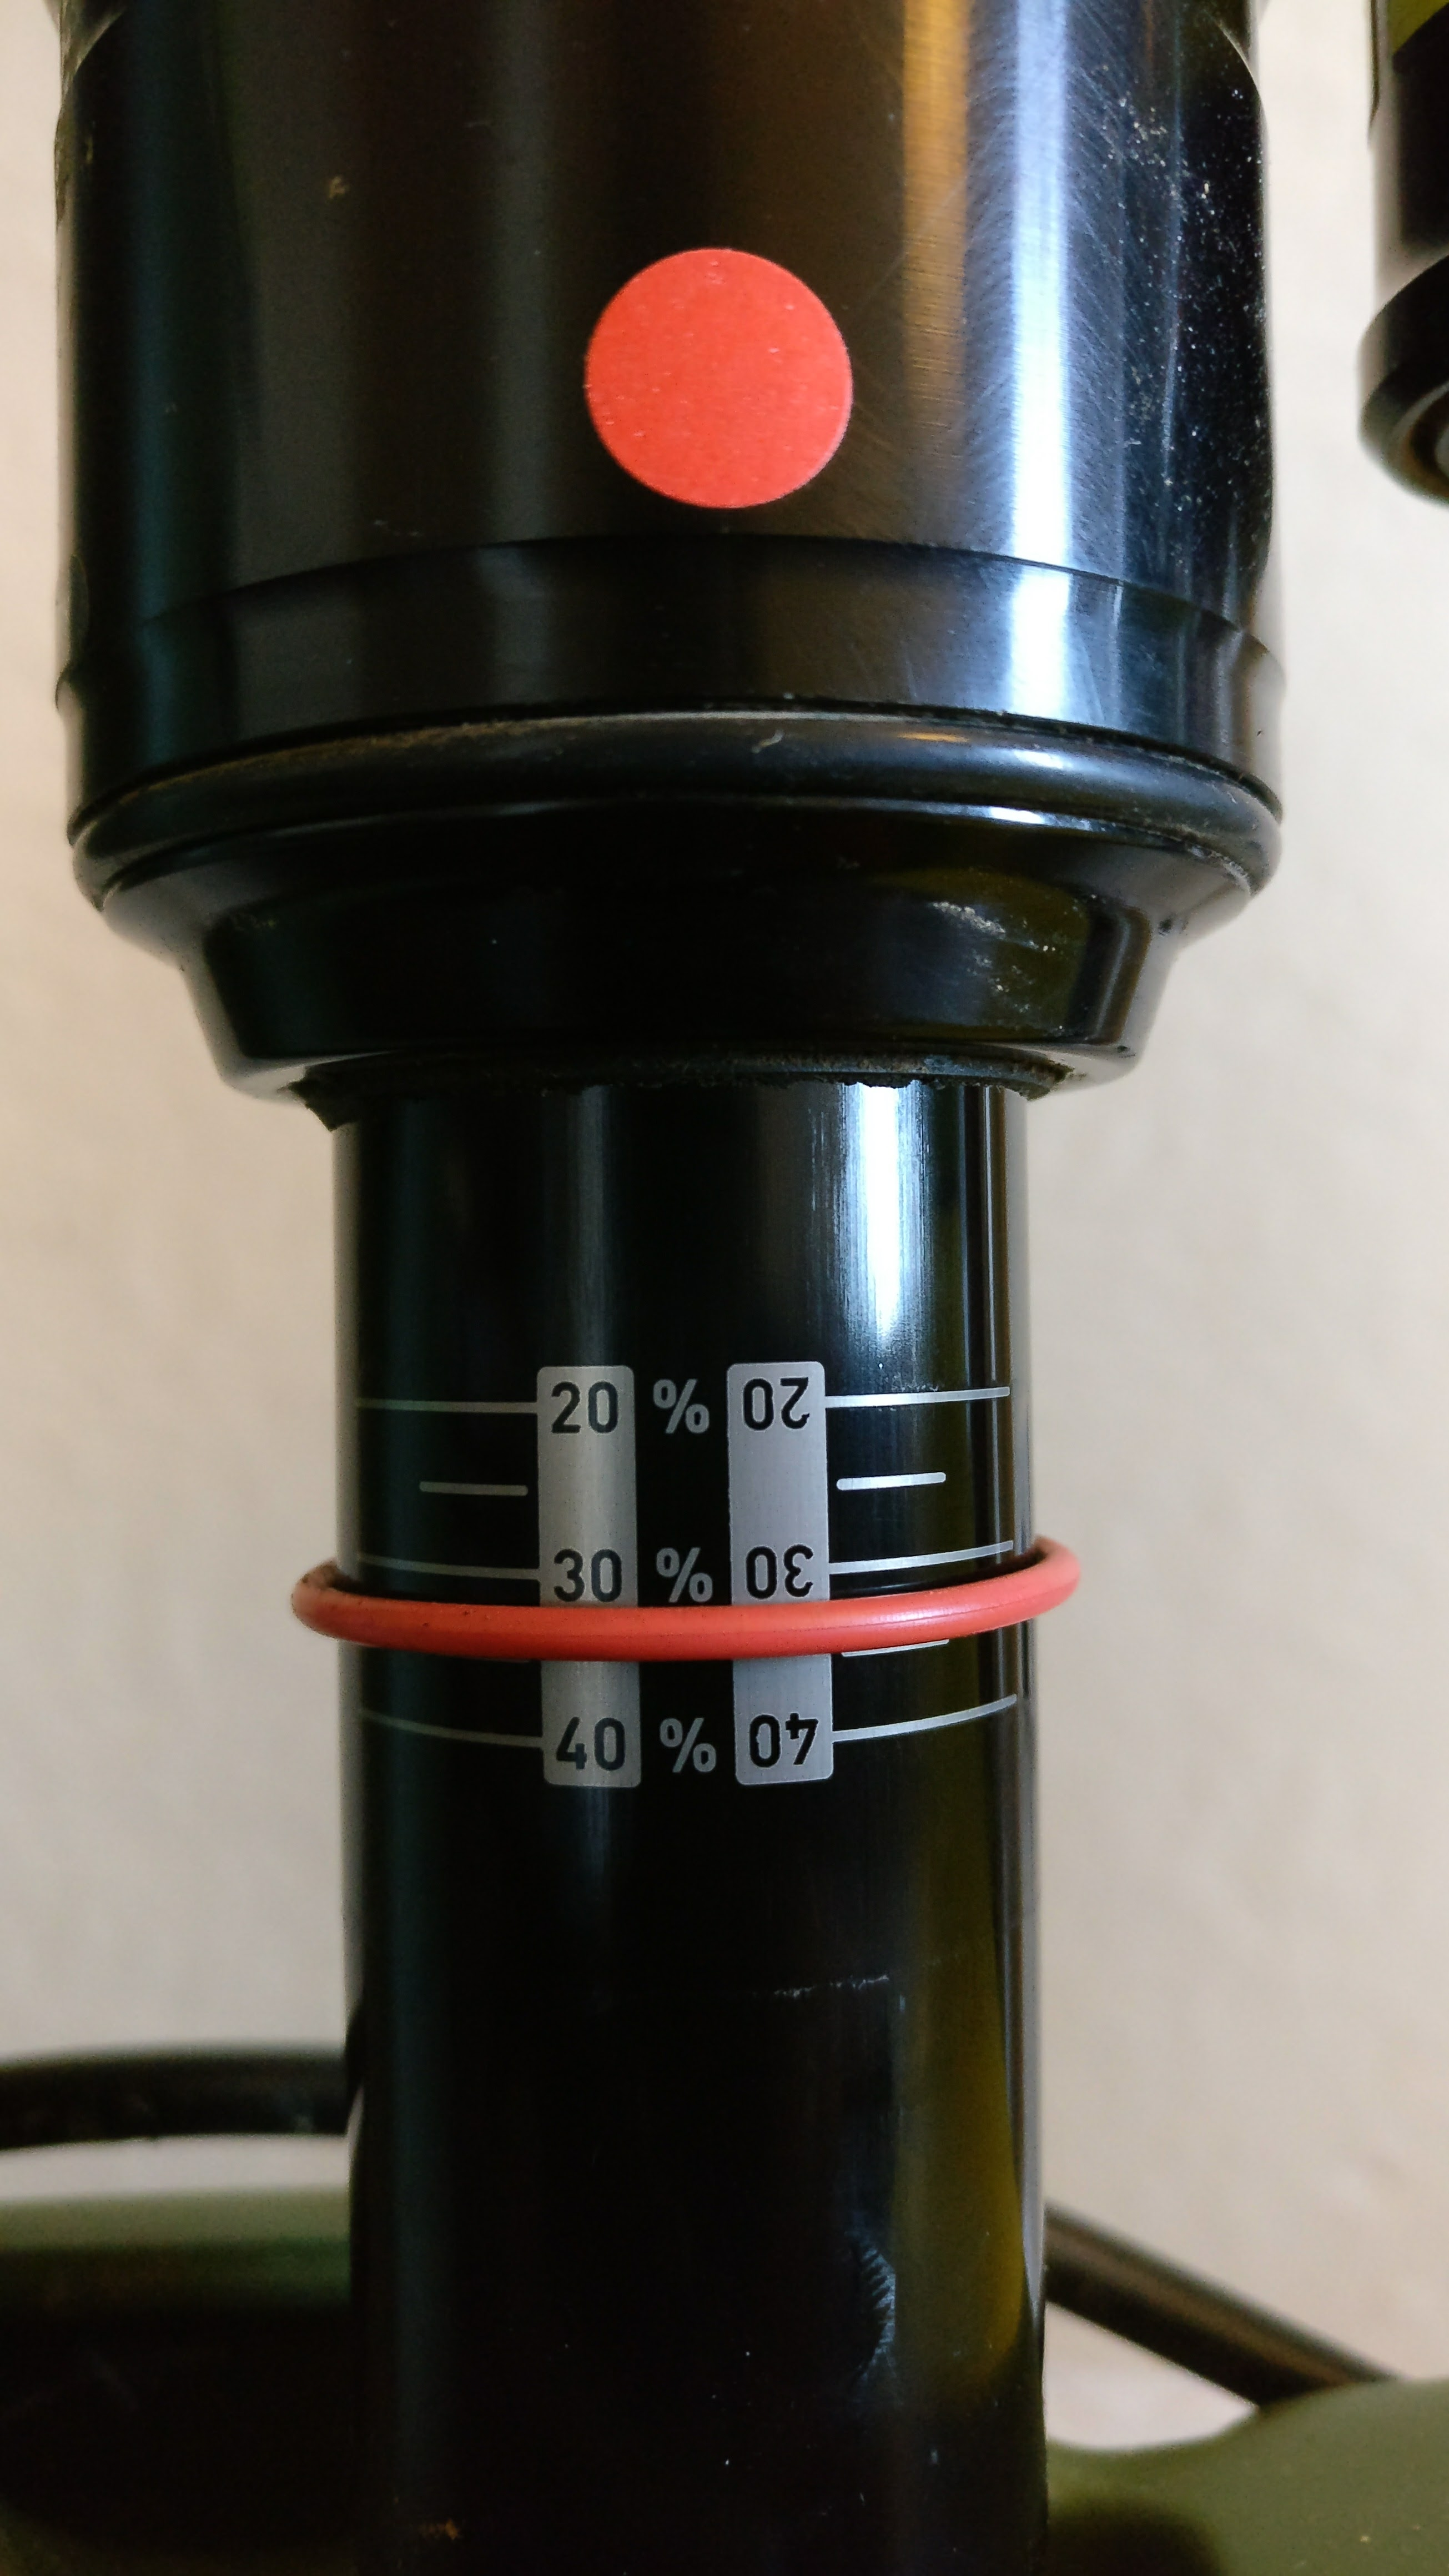
\includegraphics[scale=0.04]{../images/results/150_rs.jpg}
				\end{subfigure}
				\caption{Images suitable for processing}
				\label{fig:application_images}
			\end{figure}
		\subsubsection{Arguments}
			The application operates from a command line interface allowing the user to supply data through arguments; these are described in Table \ref{tab:arguments}. This system uses Python's Argparse package and a full command to run the application would be as follows:
			{\centering \ttfamily program -i user/images/100.jpg user/images/150.jpg -s 30 -t 57 -c red}
			\rowcolors{2}{gray!25}{white}
			\begin{table}[h!]
				\centering
				\caption{Table of application arguments}
				\label{tab:arguments}
				\begin{tabular}{|l|p{0.35\columnwidth}|p{0.25\columnwidth}|}
					\hline
					\rowcolor{gray!50}
					\bfseries Argument&\bfseries Description&\bfseries Usage\\
					\hline
					{\ttfamily -i,--image <path1 path2>}&The paths to the two images to be used for analysis&{\ttfamily -i path/to/img/1 path/to/img/2}\\
					{\ttfamily -s,--sag <percentage>}&The desired sag percentage&{\ttfamily -s 30}\\
					{\ttfamily -t,--stroke}&The stroke length of the shock being analysed&{\ttfamily -t 57}\\
					{\ttfamily -c,--colour}&The colour of the marker O-ring&{\ttfamily -c red}\\
					{\ttfamily -d,--debug}&This produces outputs from each stage to the terminal for debugging purposes&\\
					\hline
				\end{tabular}
			\end{table}
		\subsubsection{Processing}
			All source code for the application can be seen in appendix \ref{app:source}.
			\paragraph{Reference Point}
				The first process which the application must complete is to find the reference point for measurement. This is done by first colour quantifying the image to 8 bit colour so that the reference point becomes uniform in colour. The result of this process is shown in Figure \ref{subfig:quantified}. So the application can find the red colour of the reference point within the entire image, a mask is applied for any colour within a range. The output of this process is shown in Figure \ref{subfig:mask}. If an alternative colour reference point were to be used, this colour range could be easily adapted.
				\\\\
				The contours, or shapes in this image are then found and sorted by their area in decreasing order. By doing this it can be assumed with a high level of confidence that the largest will be the reference point. The found contour can be seen in Figure \ref{subfig:contours}. A bounding circle is created around the reference point contour, as shown in Figure \ref{subfig:boundaries}, and this can be used to calculate the pixel per millimetre metric.
			\begin{figure}[h!]
				\centering
				\begin{subfigure}[t]{0.2\textwidth}
					\centering
					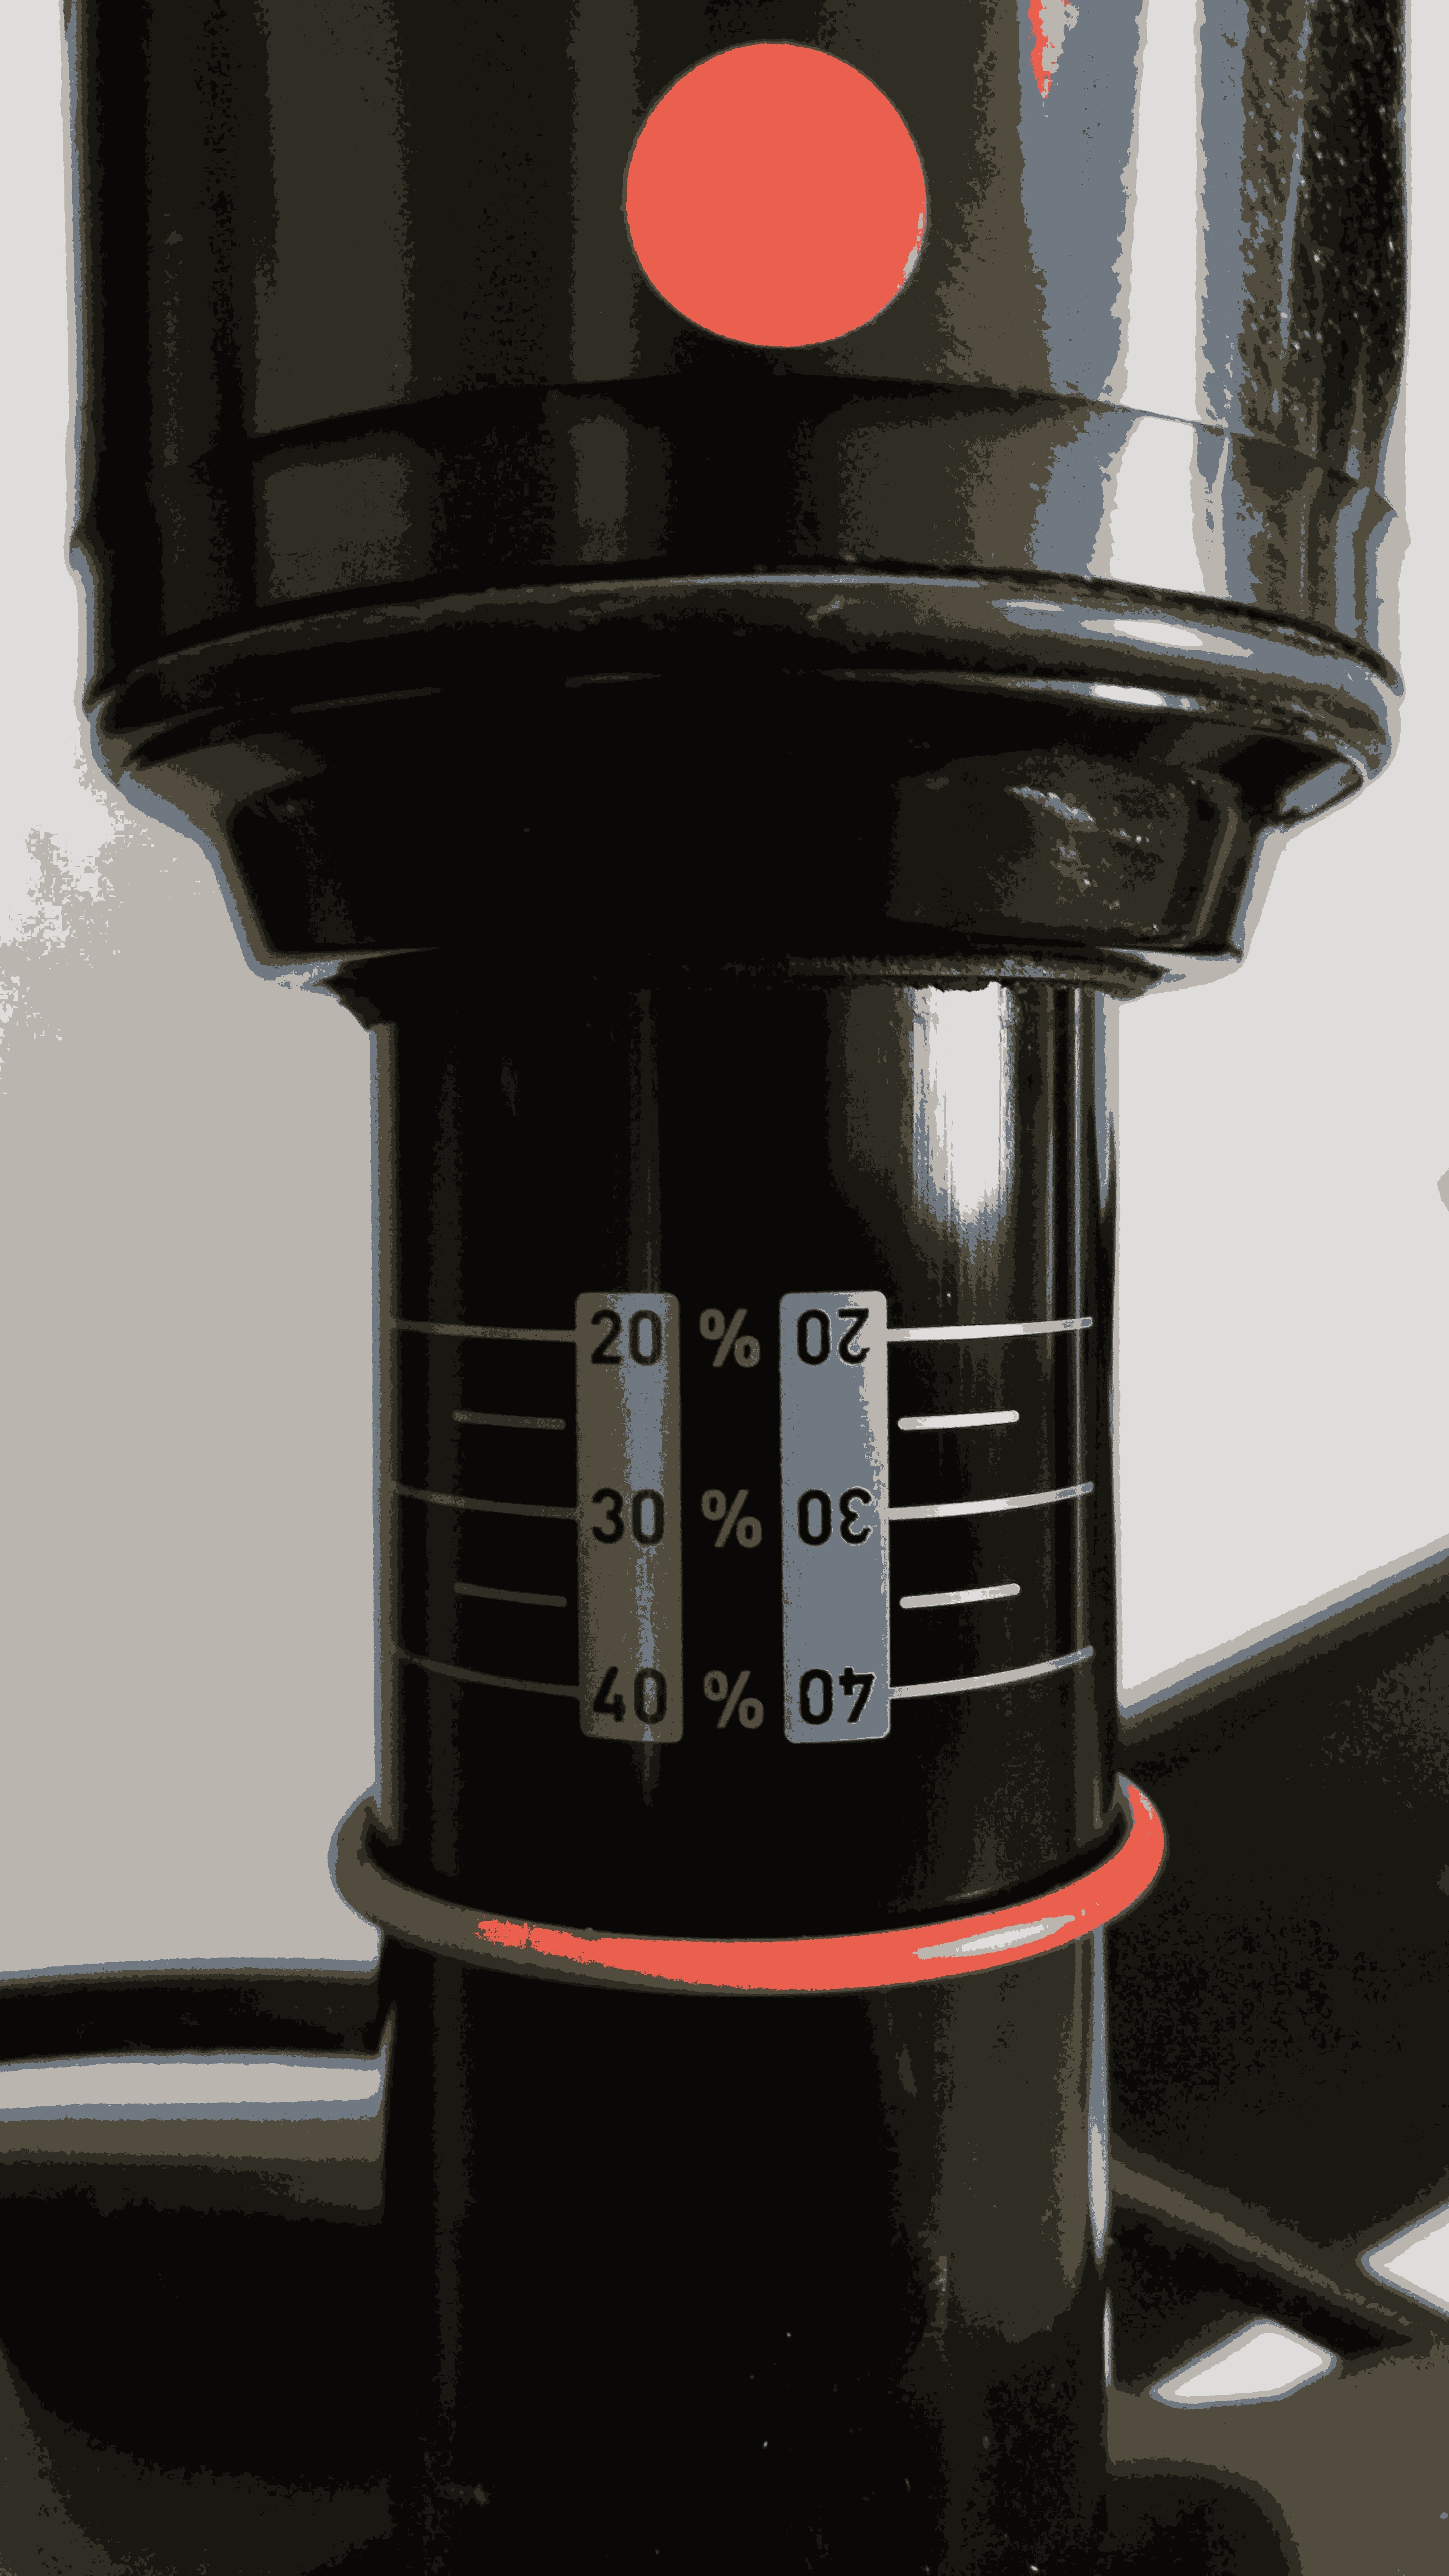
\includegraphics[scale=0.04]{../images/results/quant.jpg}
			 		\subcaption{Colour quantified image}
					\label{subfig:quantified}
				\end{subfigure}\hfill
				\begin{subfigure}[t]{0.2\textwidth}
					\centering
					
\includegraphics[scale=0.04]{../images/results/mask.jpg}
					\subcaption{Red image mask}
					\label{subfig:mask}
				\end{subfigure}\hfill
				\begin{subfigure}[t]{0.2\textwidth}
					\centering
					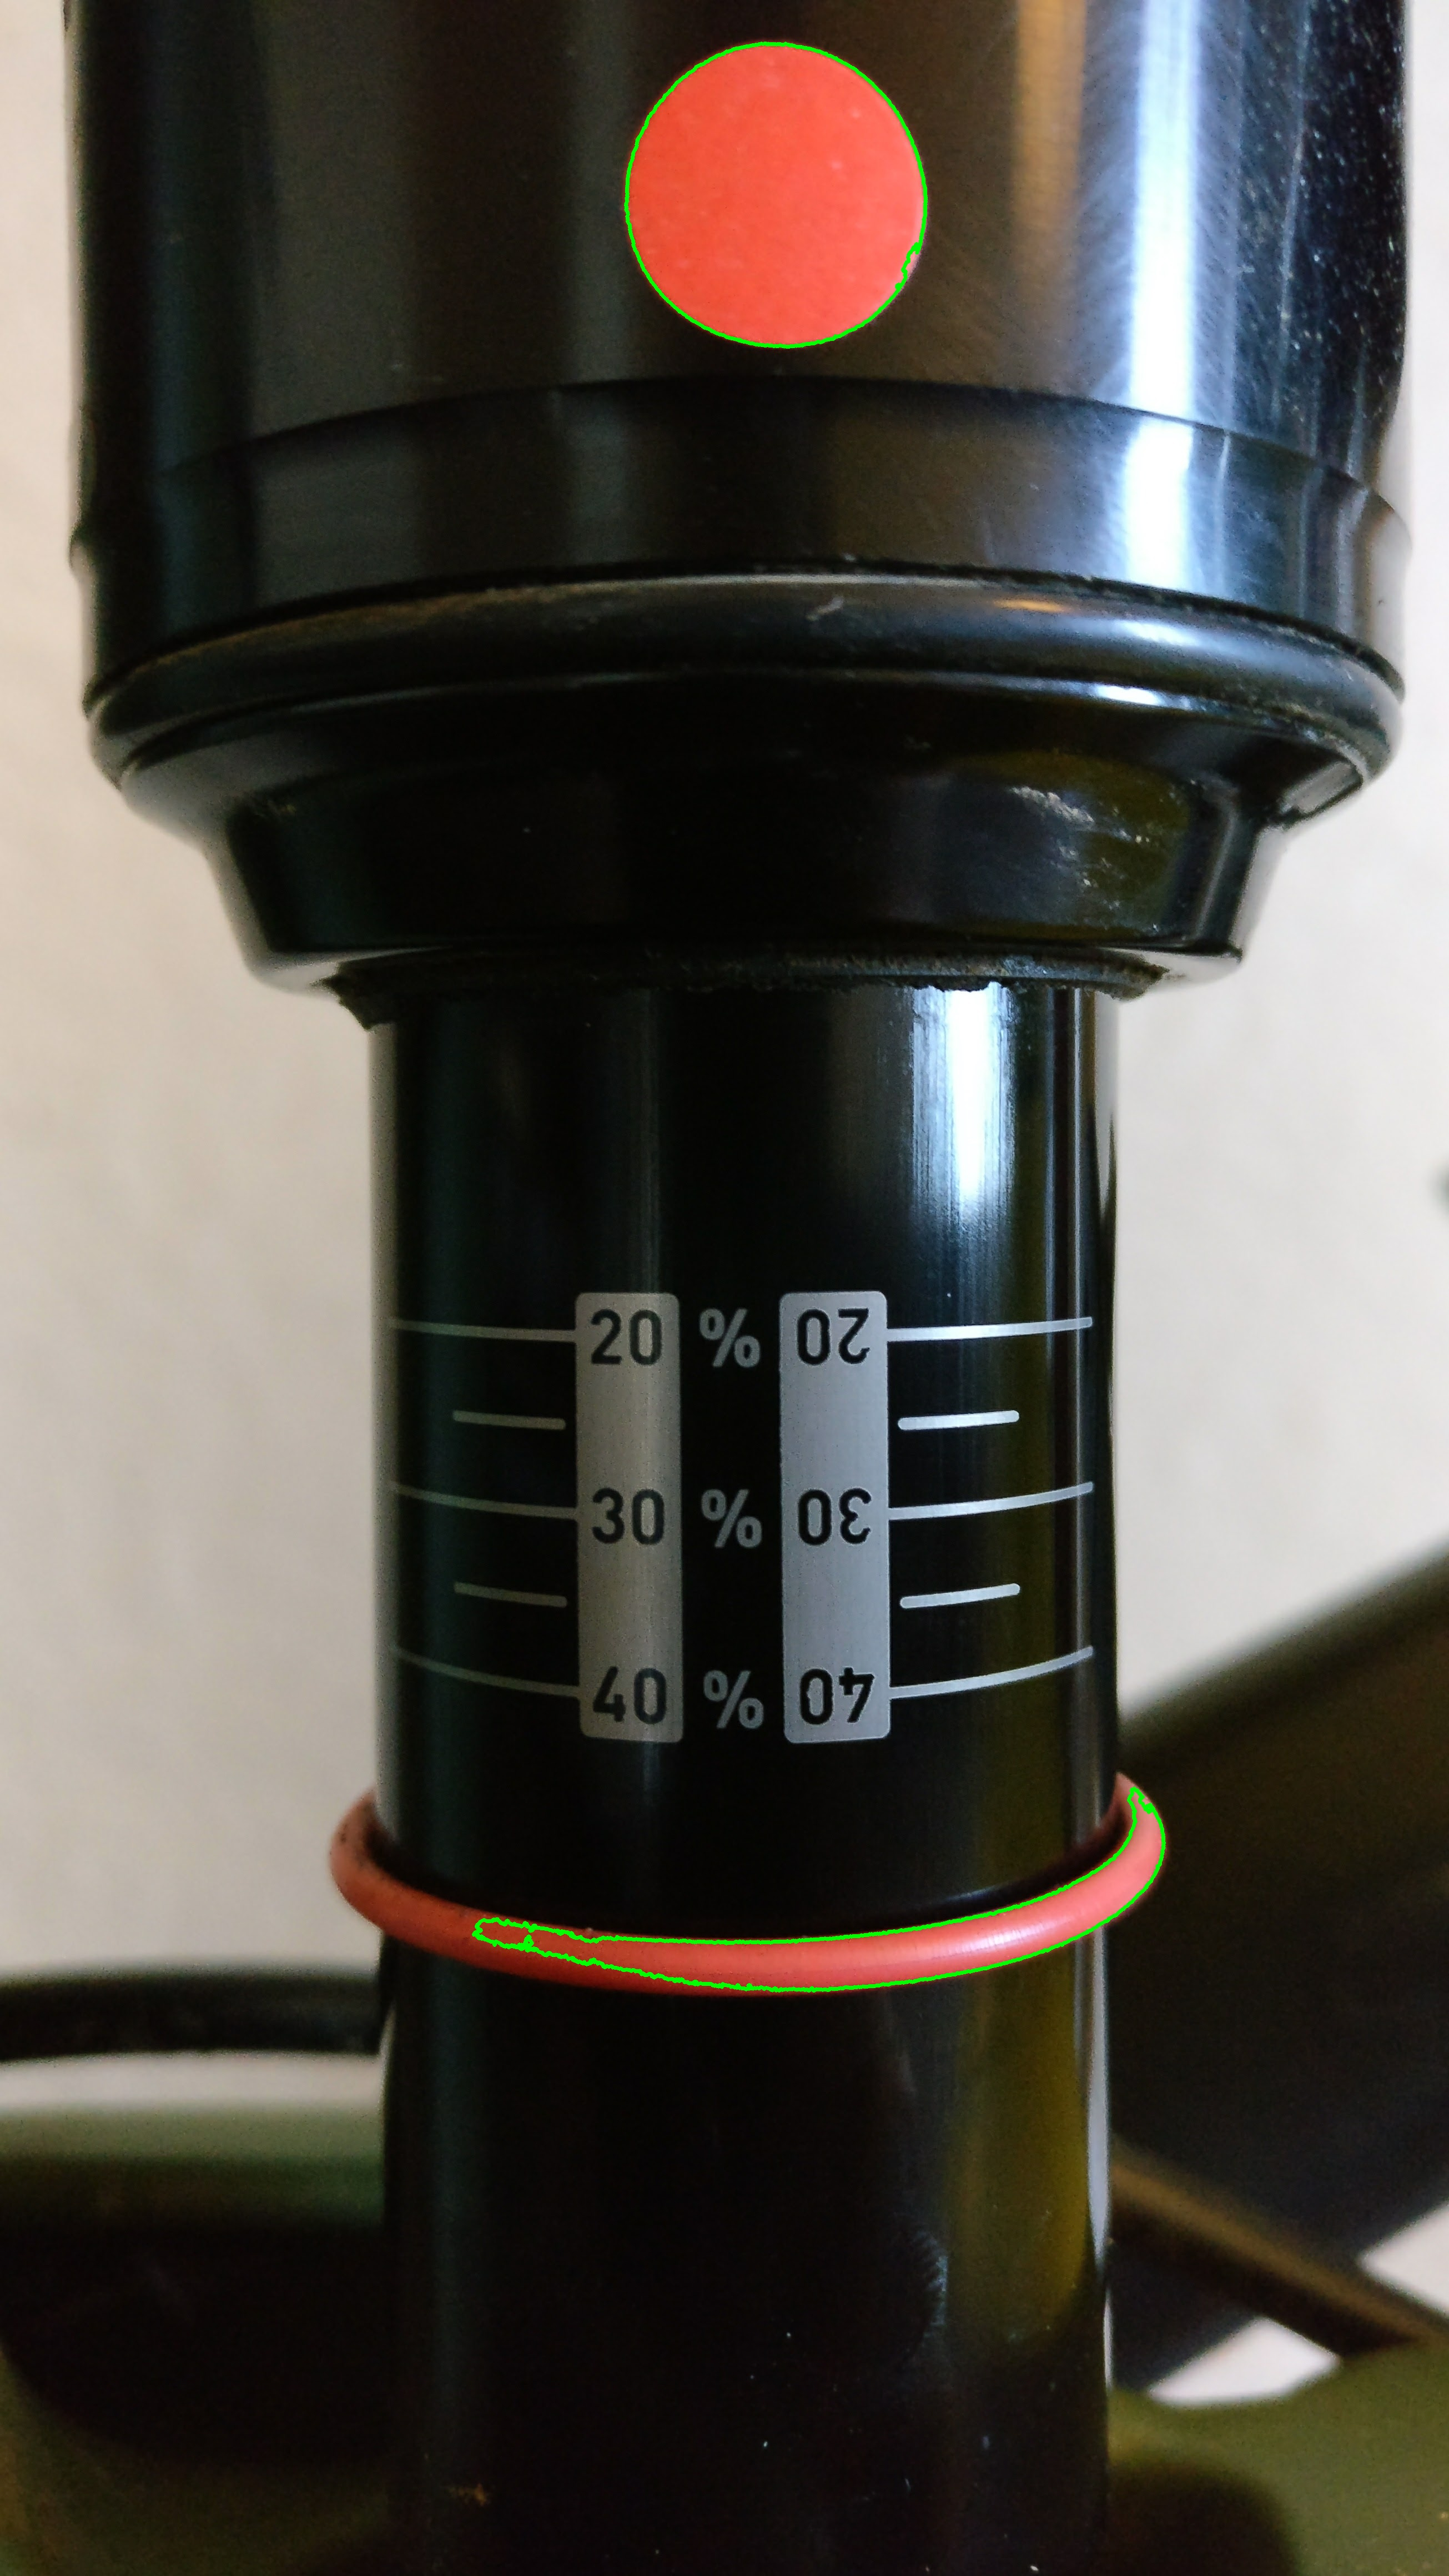
\includegraphics[scale=0.04]{../images/results/contours.jpg}
					\subcaption{Found contours from mask}
					\label{subfig:contours}
				\end{subfigure}\hfill
				\begin{subfigure}[t]{0.2\textwidth}
					\centering
					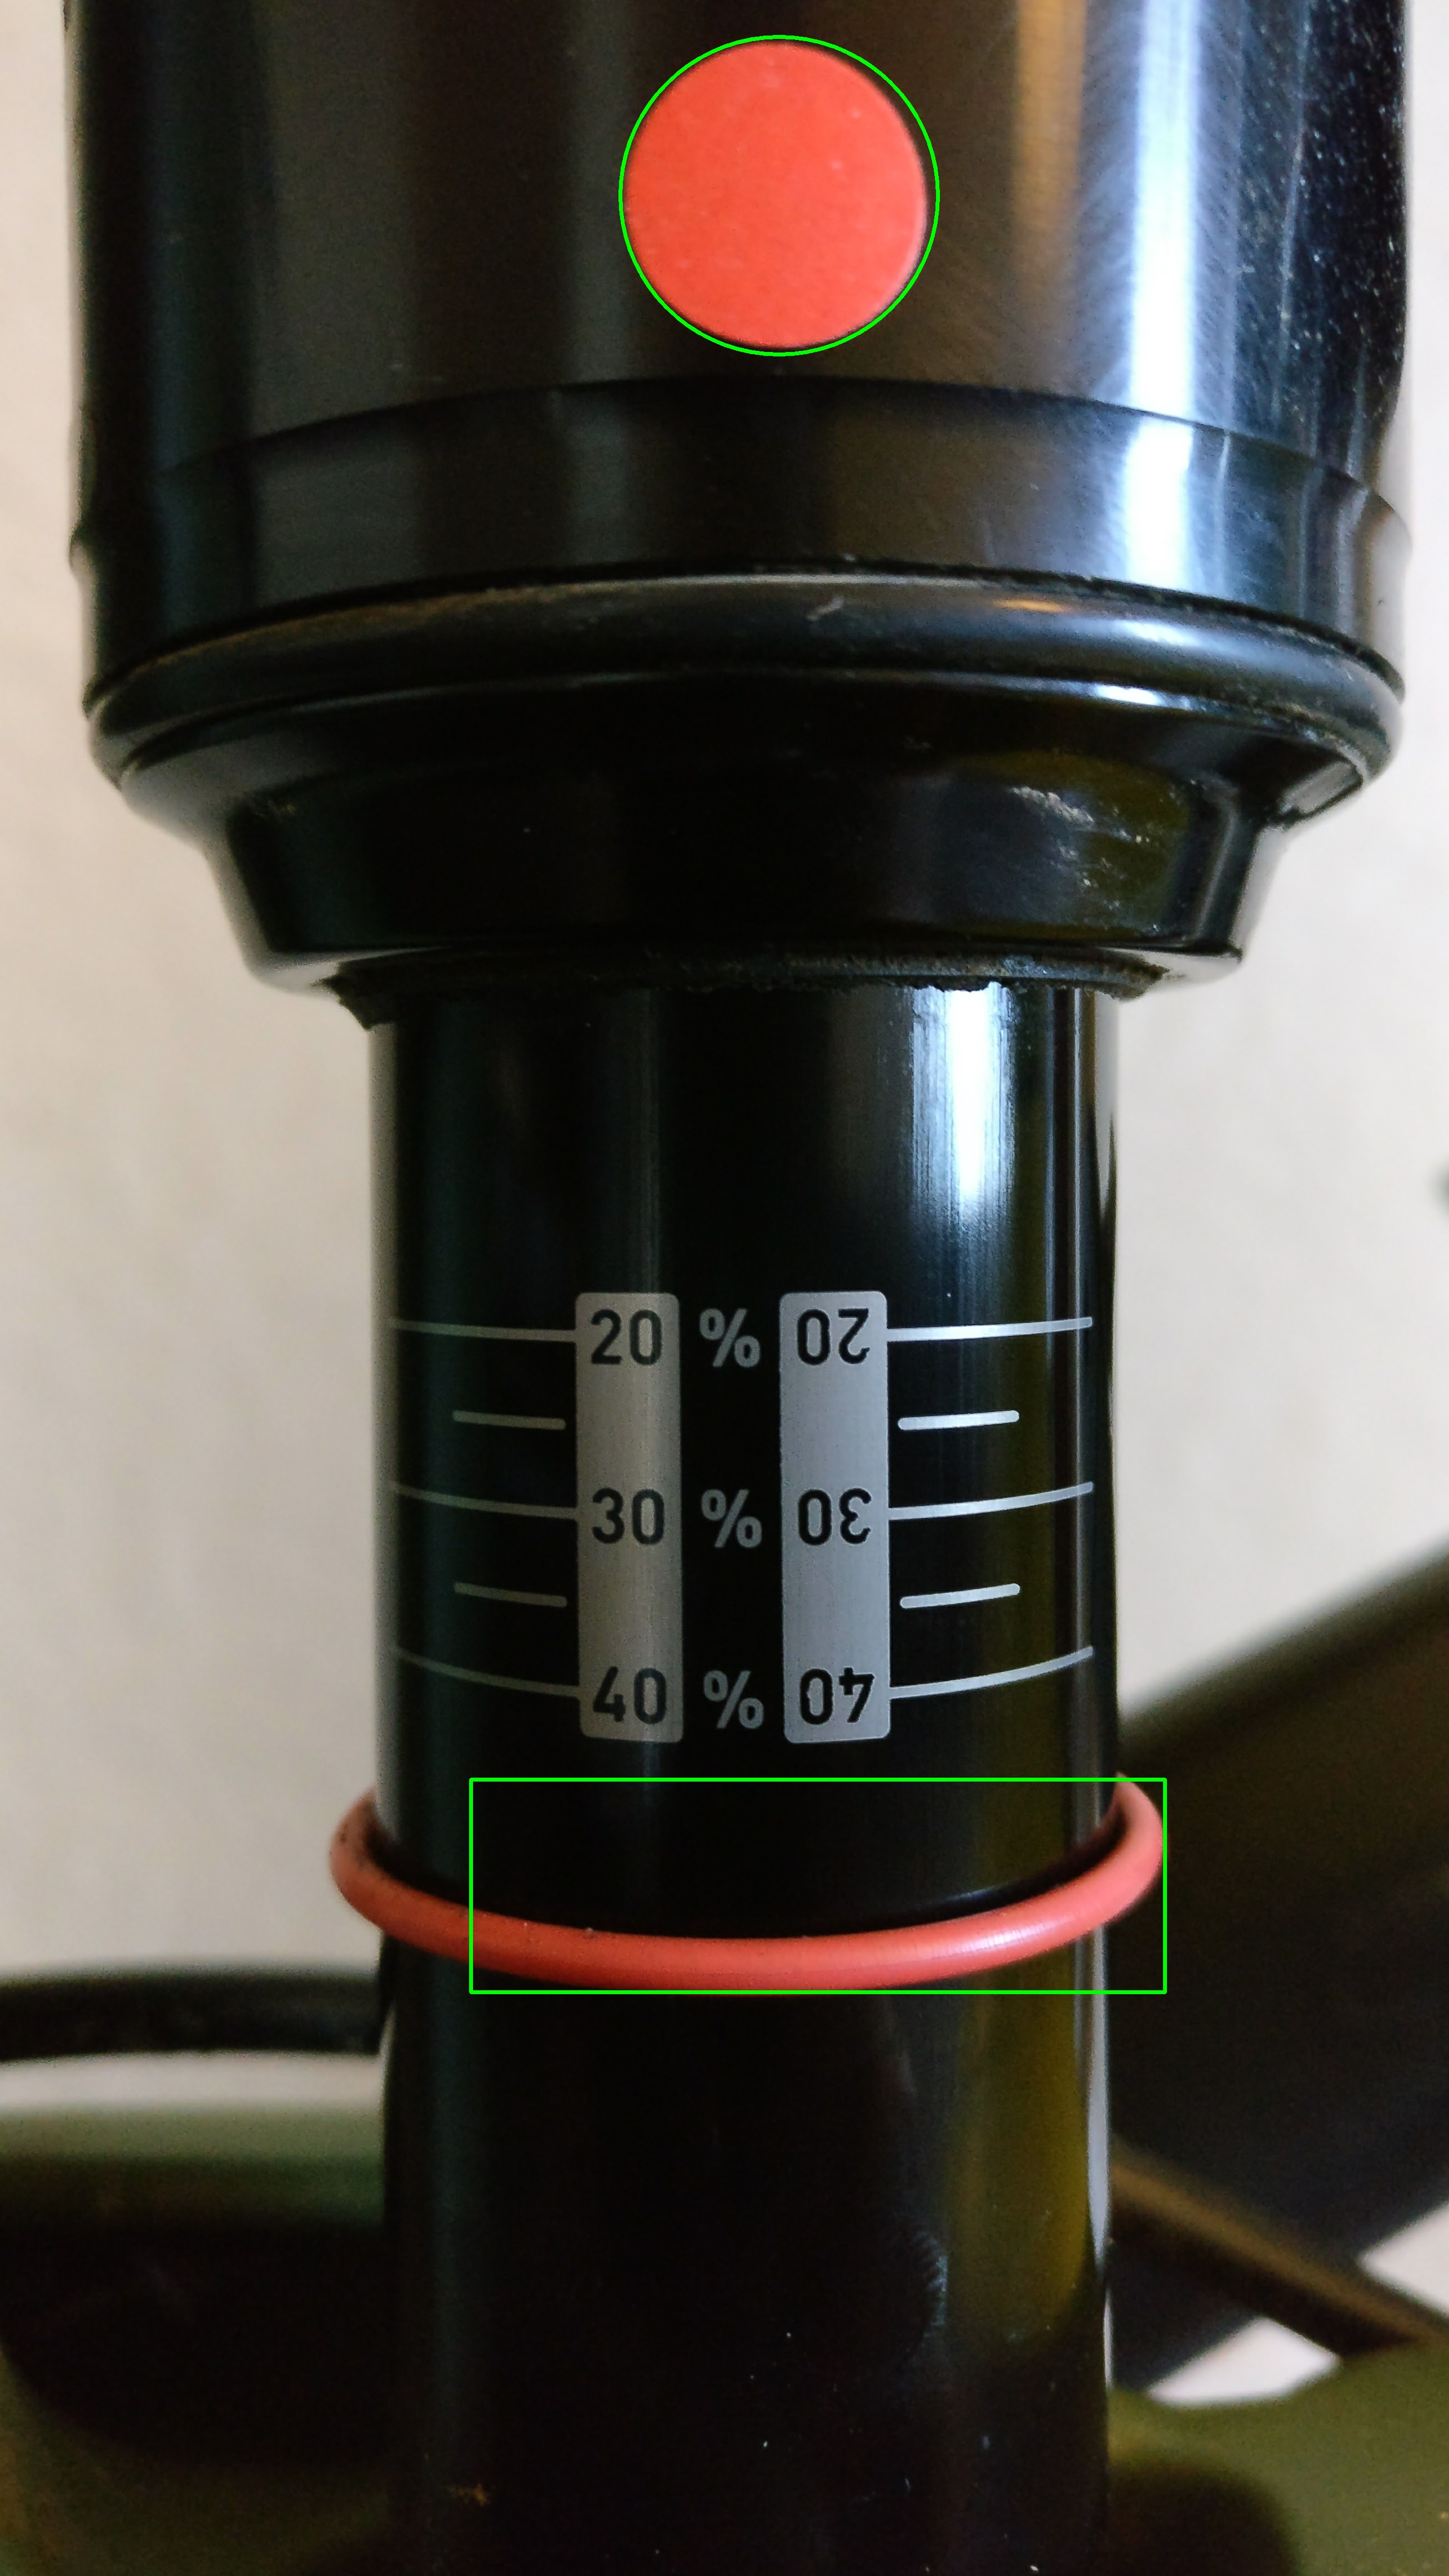
\includegraphics[scale=0.04]{../images/results/raw_refs.jpg}
					\subcaption{Bounding circle and box applied from contours}
					\label{subfig:boundaries}
				\end{subfigure}
				\caption{Processed images for finding reference point}
				\label{fig:ref_point_process}
			\end{figure}
		\paragraph{O-Ring}
			If a red coloured O-ring is specified then the same process to find the reference point is used. The second largest contour found will be the O-ring so a bounding box can be drawn round it from which a measurement limit can be collected. The red O-ring mask, contour, and bounding box can be seen in Figure \ref{fig:ref_point_process}. 
			\\\\
			If a black O-ring is specified, an alternative process is used. Thresholding is applied to the image which emphasises any shadows or highlights on the shock shaft. As these are intersected by the O-ring it is simple to select a contour which ends at the O-ring to use as a measurement limit. This process is shown in Figure \ref{fig:fox_oring}.
			\begin{figure}[h!]
				\centering
				\begin{subfigure}[t]{0.4\textwidth}
					\centering
					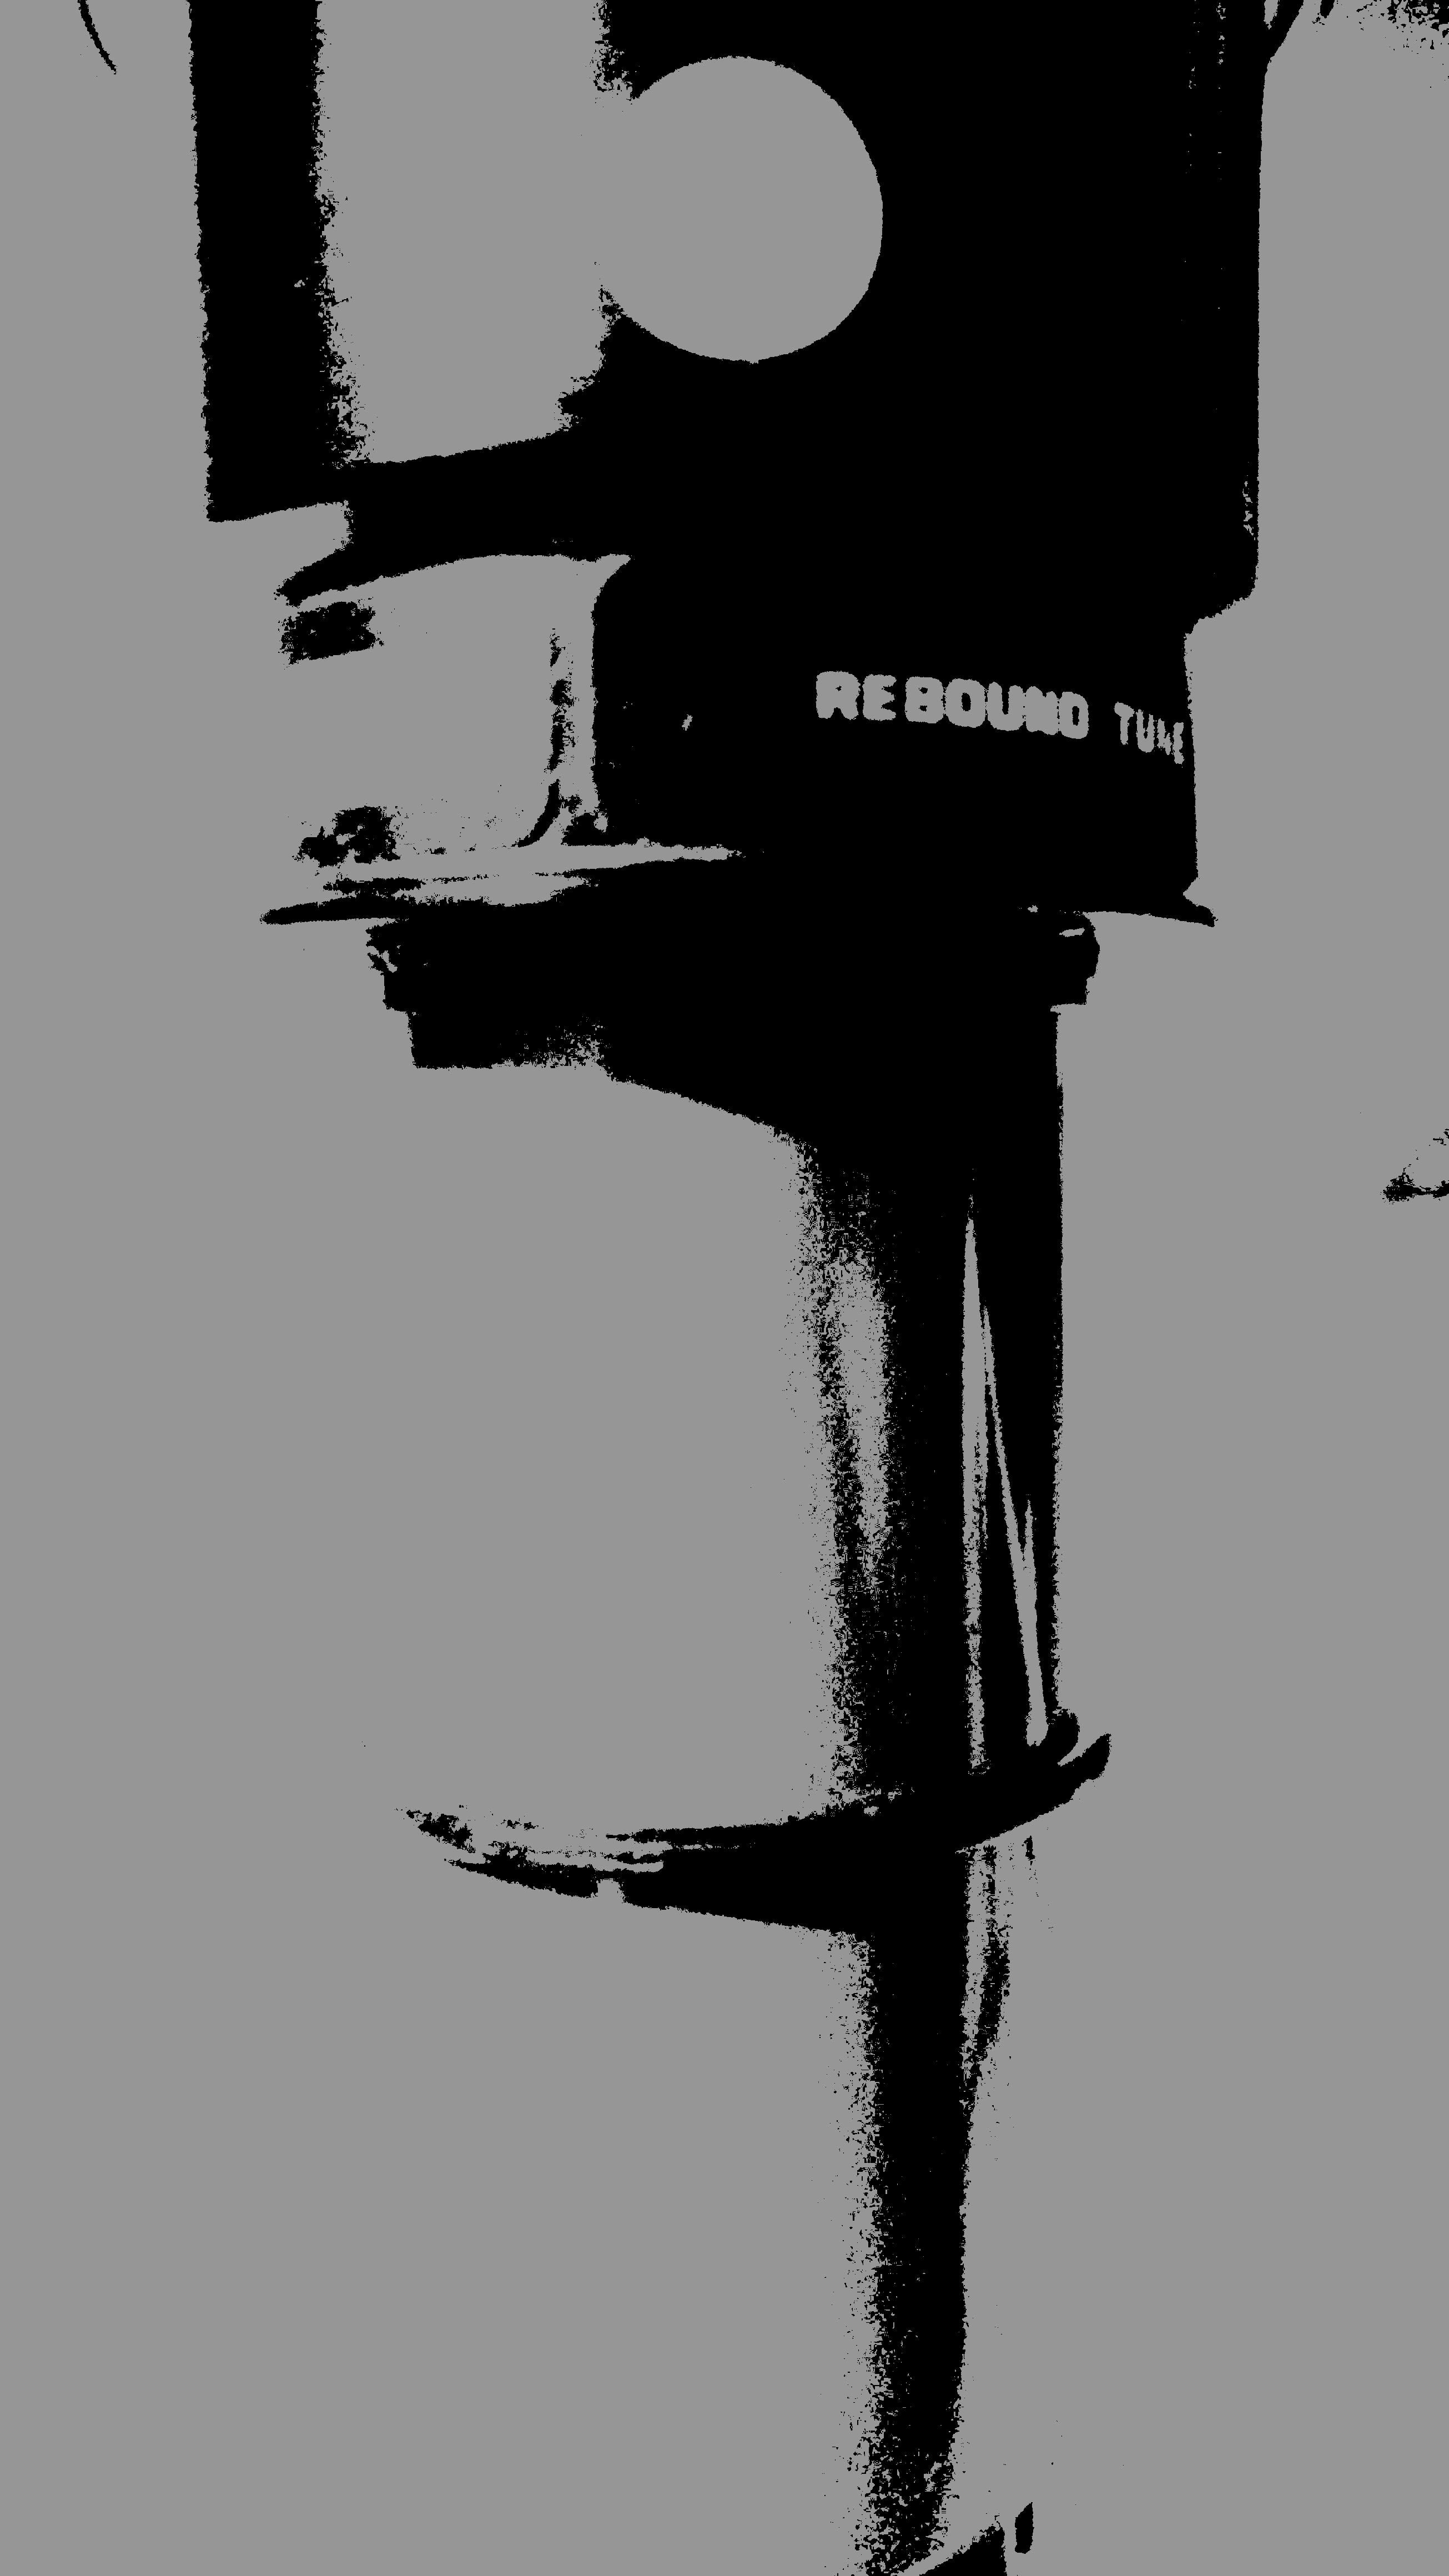
\includegraphics[scale=0.04]{../images/results/threshold.jpg}
					\subcaption{Image thresholding}
					\label{subfig:threshold}
				\end{subfigure}
				\begin{subfigure}[t]{0.4\textwidth}
					\centering
					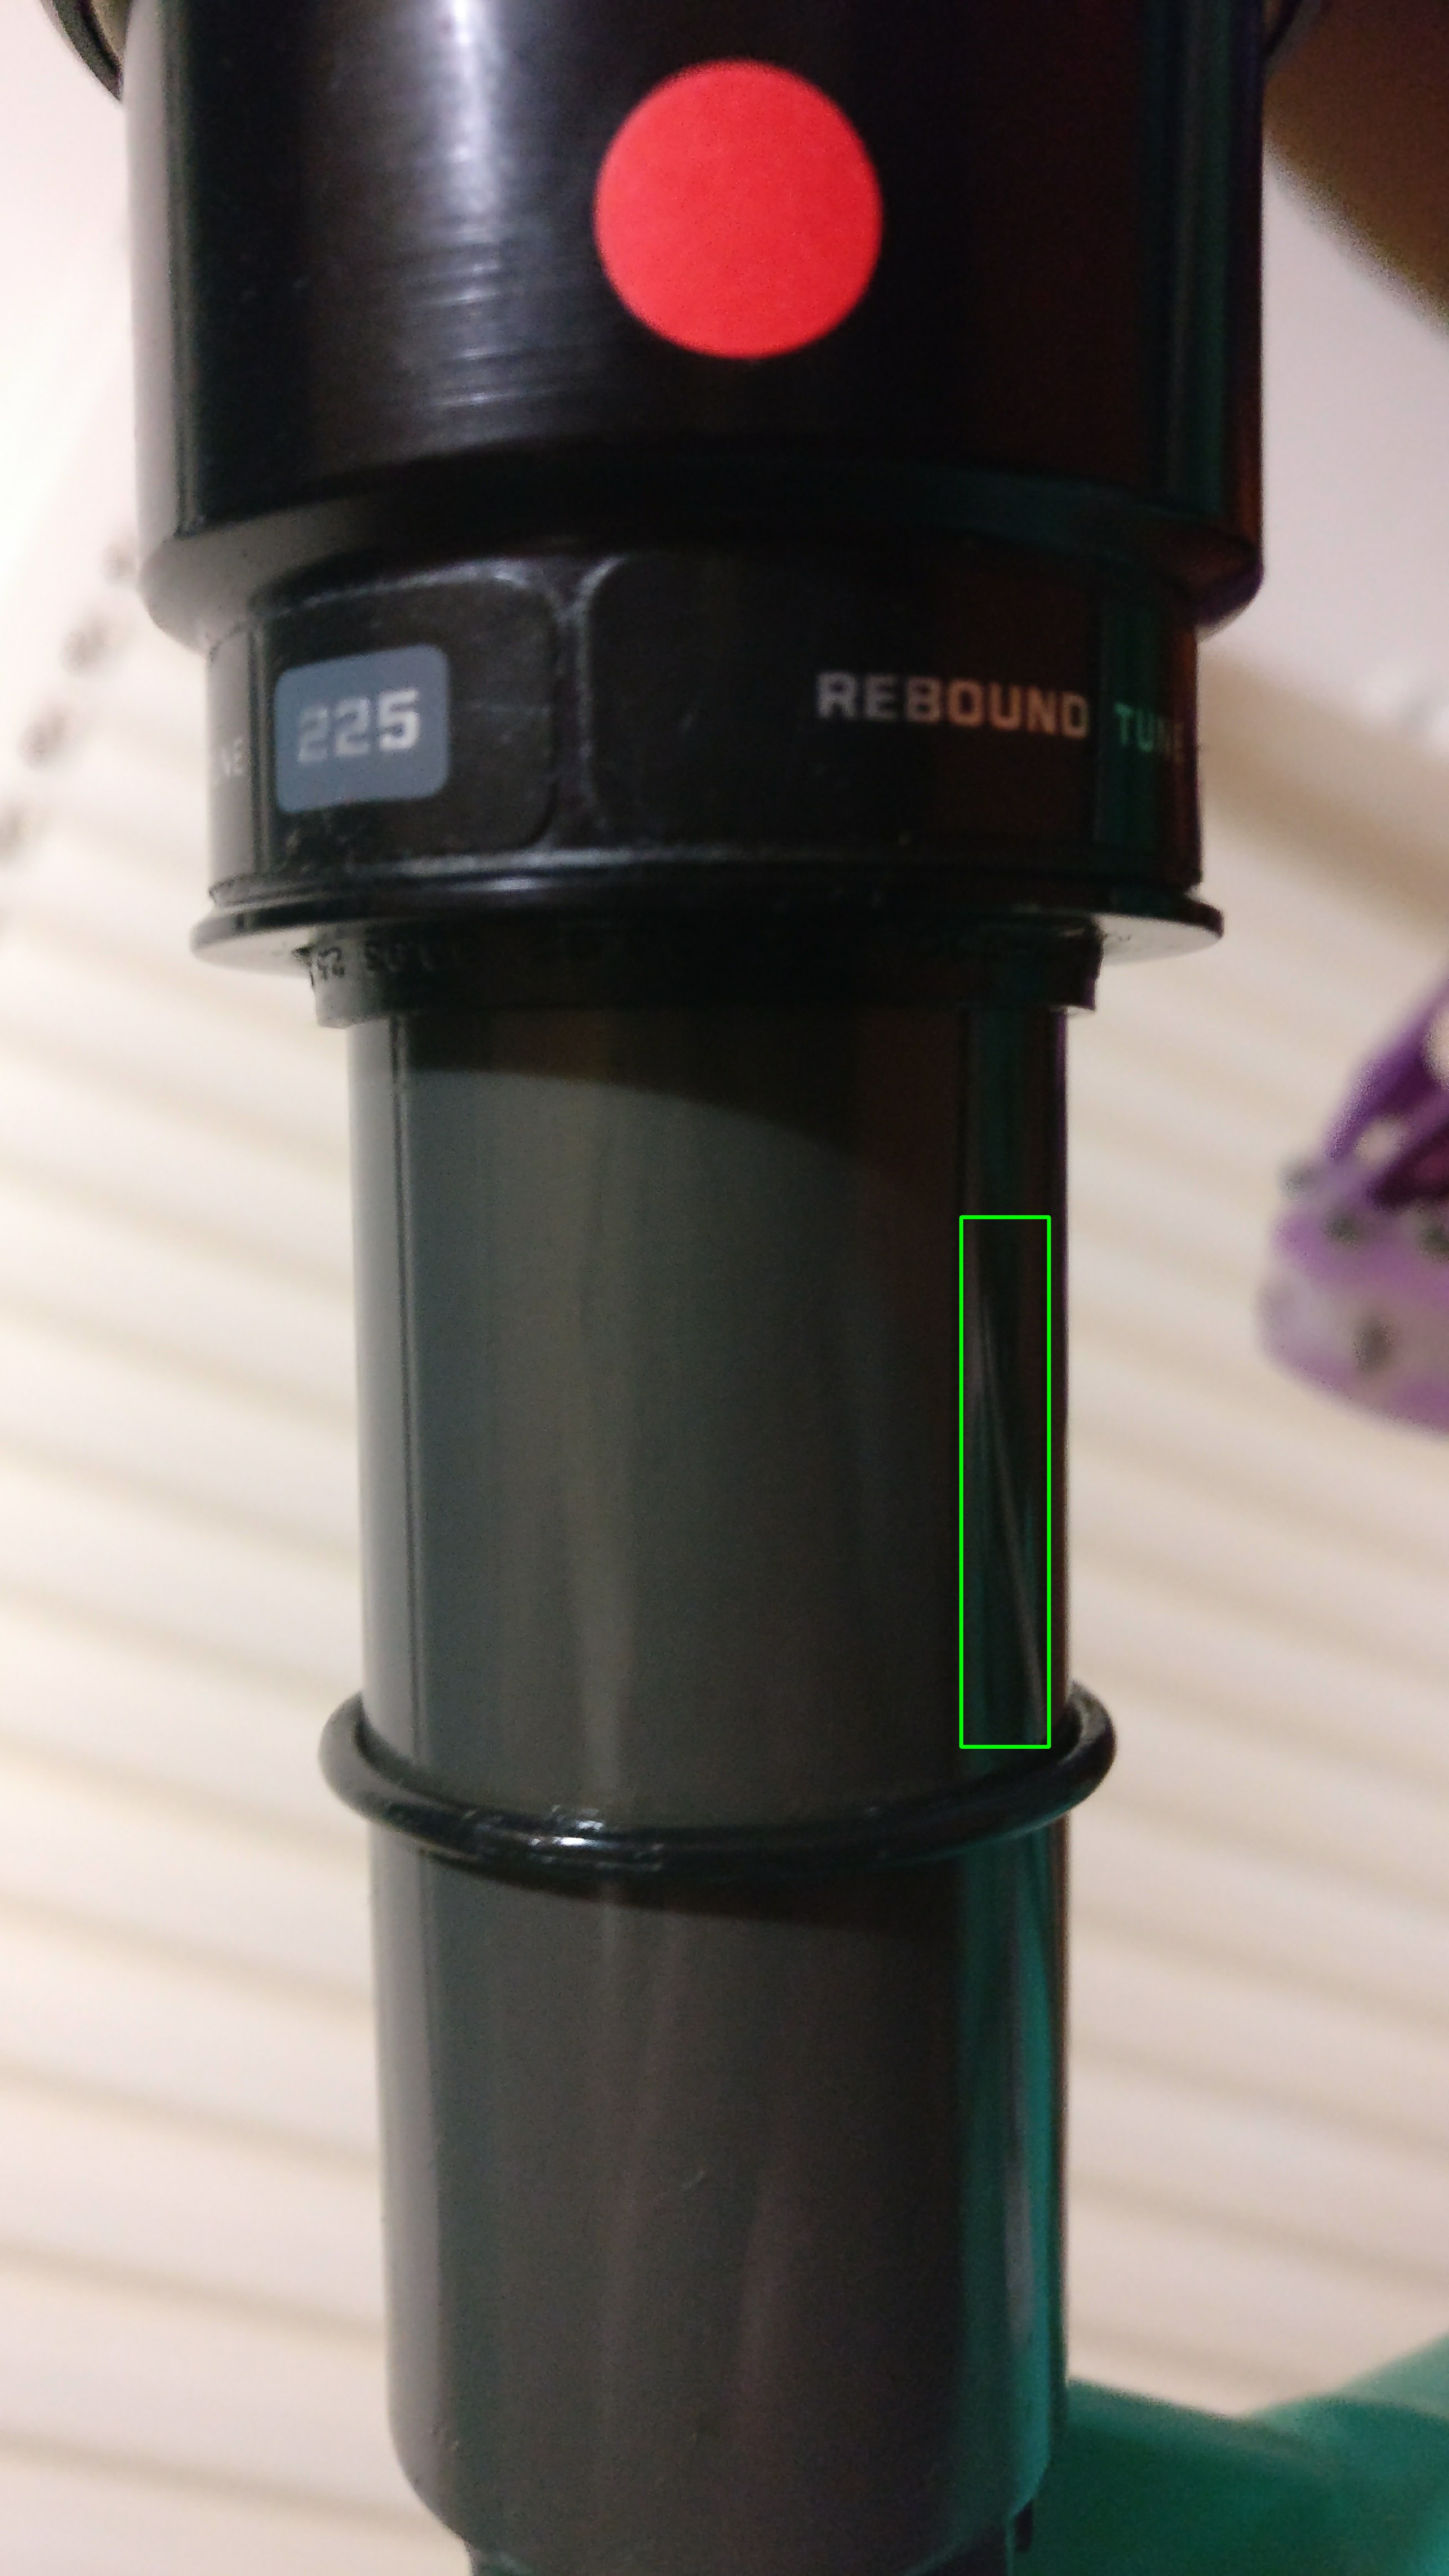
\includegraphics[scale=0.04]{../images/results/fox_oring.jpg}	
					\subcaption{O-ring indicator}
					\label{subfig:fox_oring}
				\end{subfigure}
				\caption{Locating process for black O-ring}
				\label{fig:fox_oring}
			\end{figure}
		\paragraph{Measurement}
			With the pixels per millimetre metric produced and the measurement limit found, the sag under the current pressure is measured. First, edge detection is carried out on the original input image to highlight the lines of the shock, as shown in Figure \ref{subfig:edge_detect}. Hough line transformation is then applied to locate vertical lines between the top of the shock shaft and the measurement limit. The difference in pixel count between the highest and lowest points of these lines represents the current sag measurement in the image and this can be converted to millimetres using the px/mm metric.
			\begin{figure}[h!]
				\centering
				\begin{subfigure}[t]{0.4\textwidth}
					\centering
					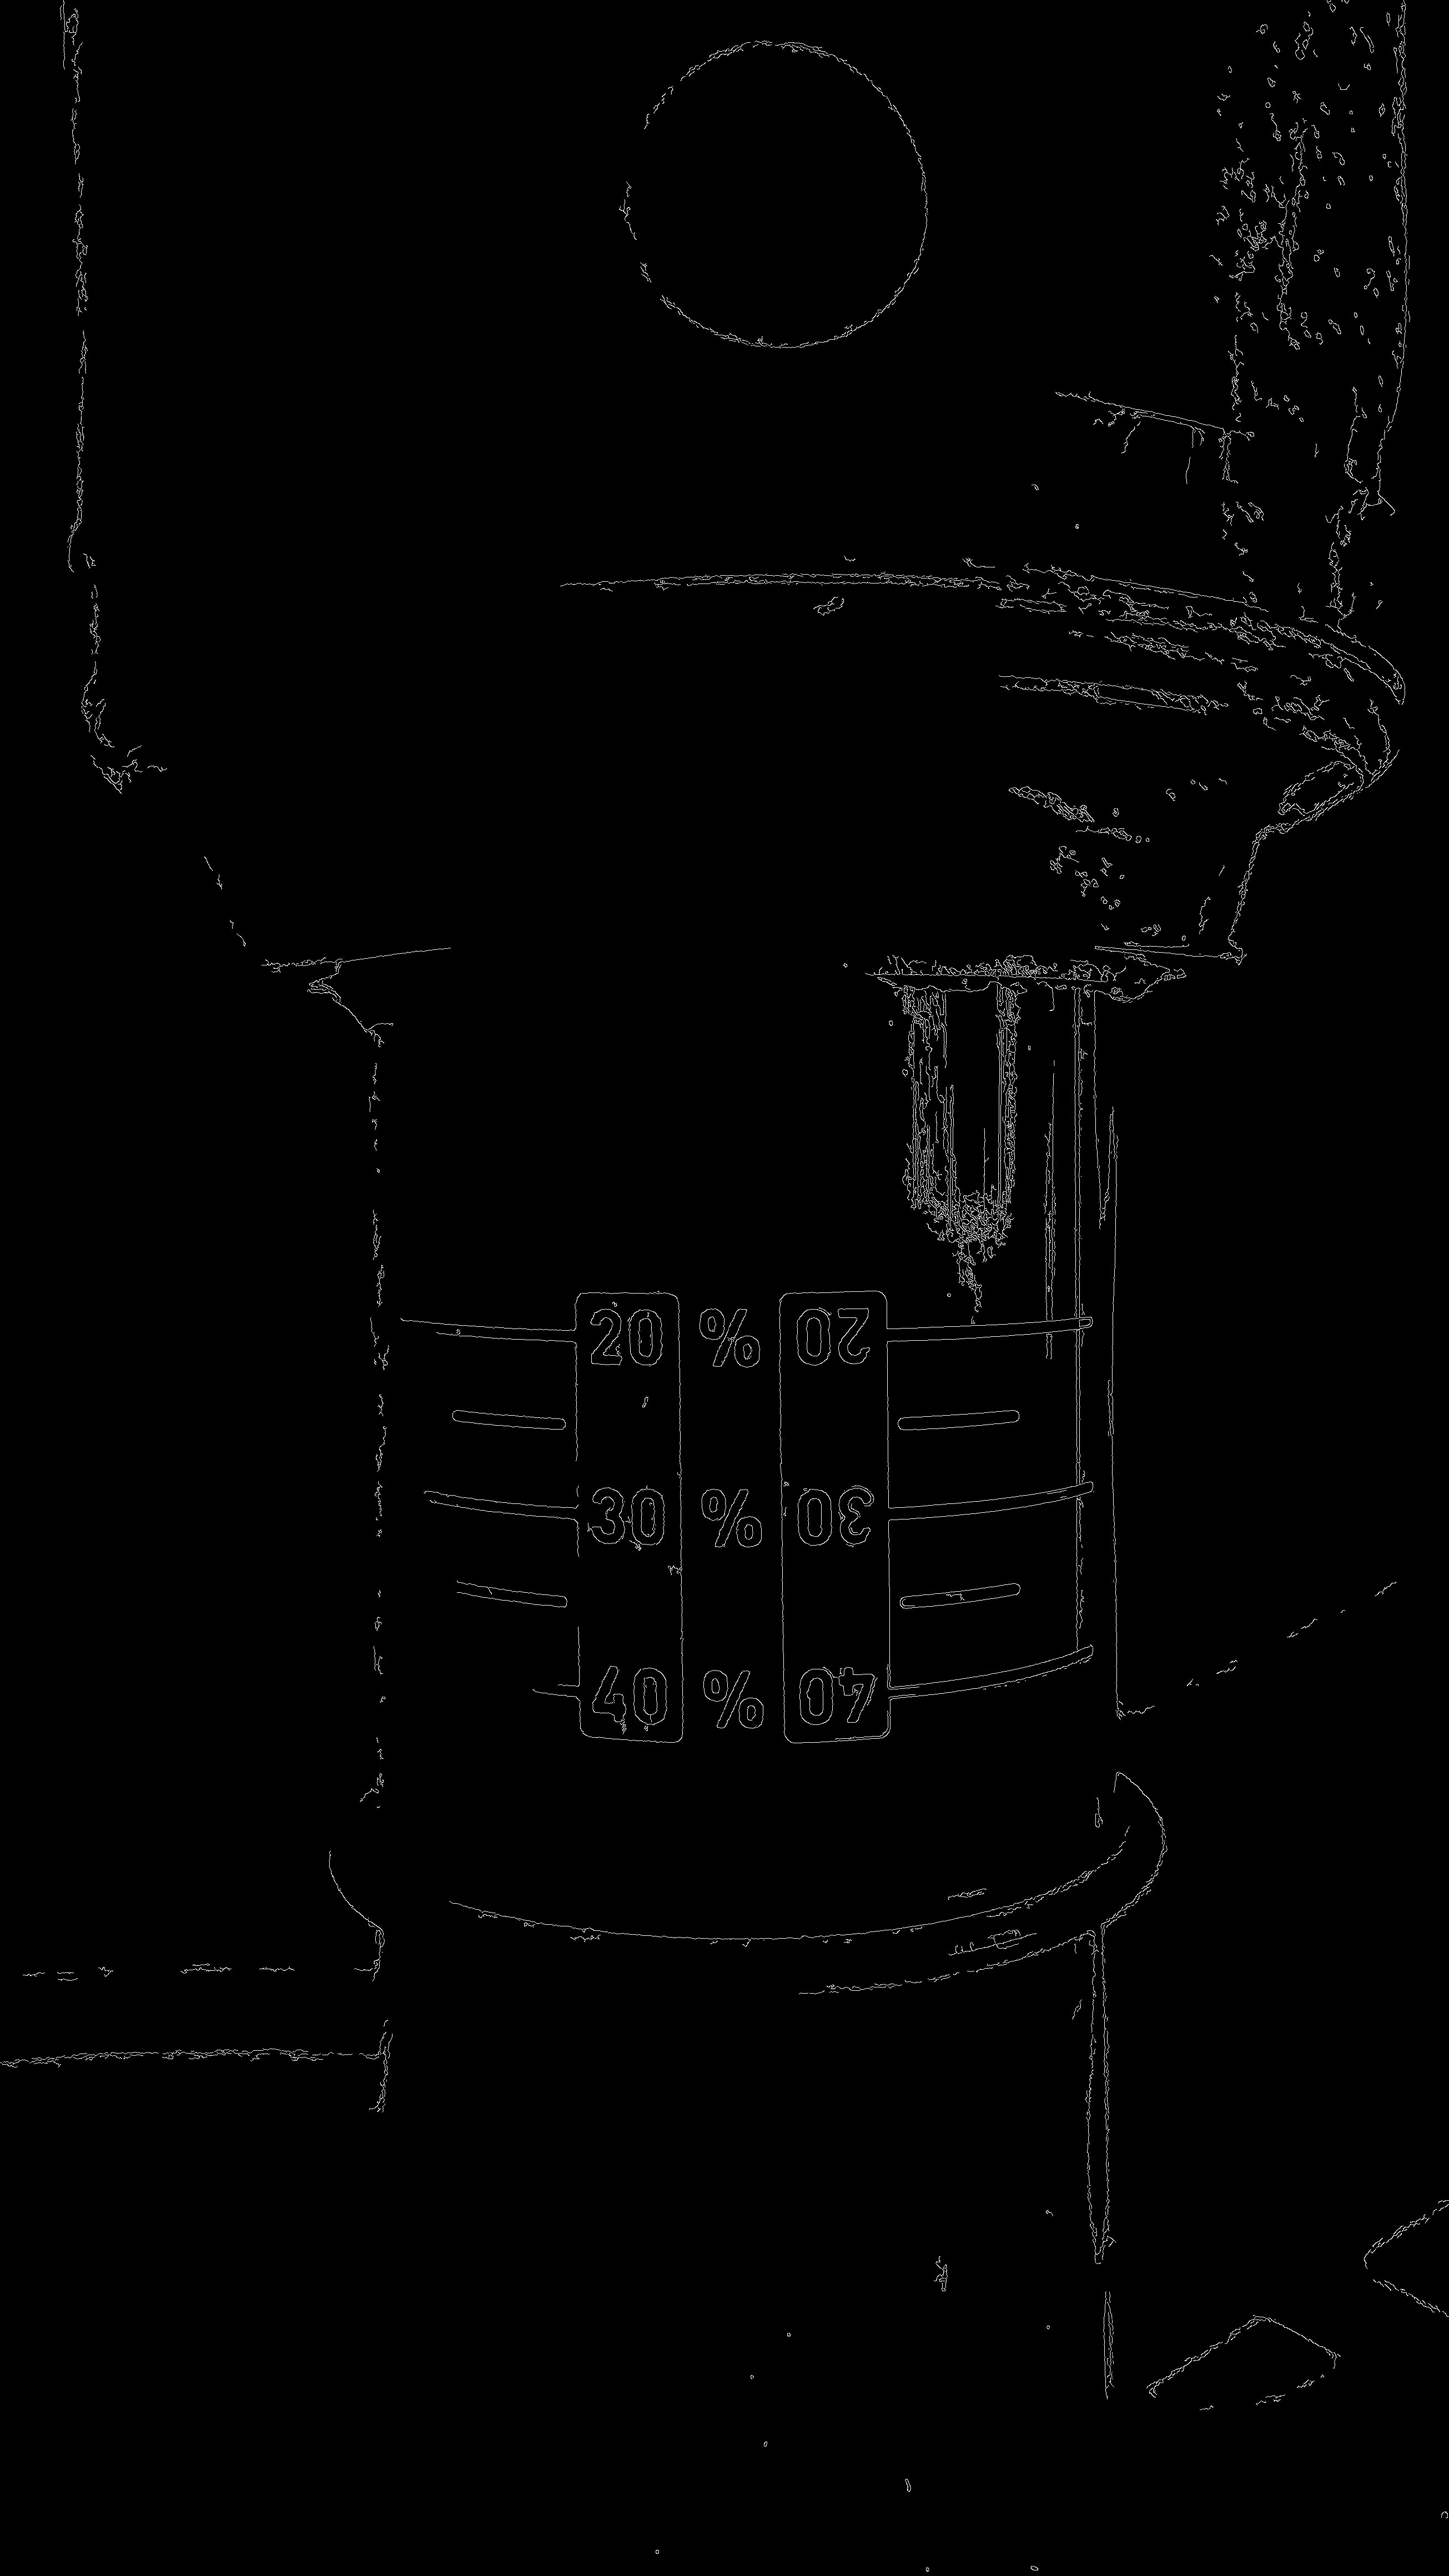
\includegraphics[scale=0.04]{../images/results/edged.jpg}
					\caption{Edge detected image}
					\label{subfig:edge_detect}
				\end{subfigure}
				\begin{subfigure}[t]{0.4\textwidth}
					\centering
					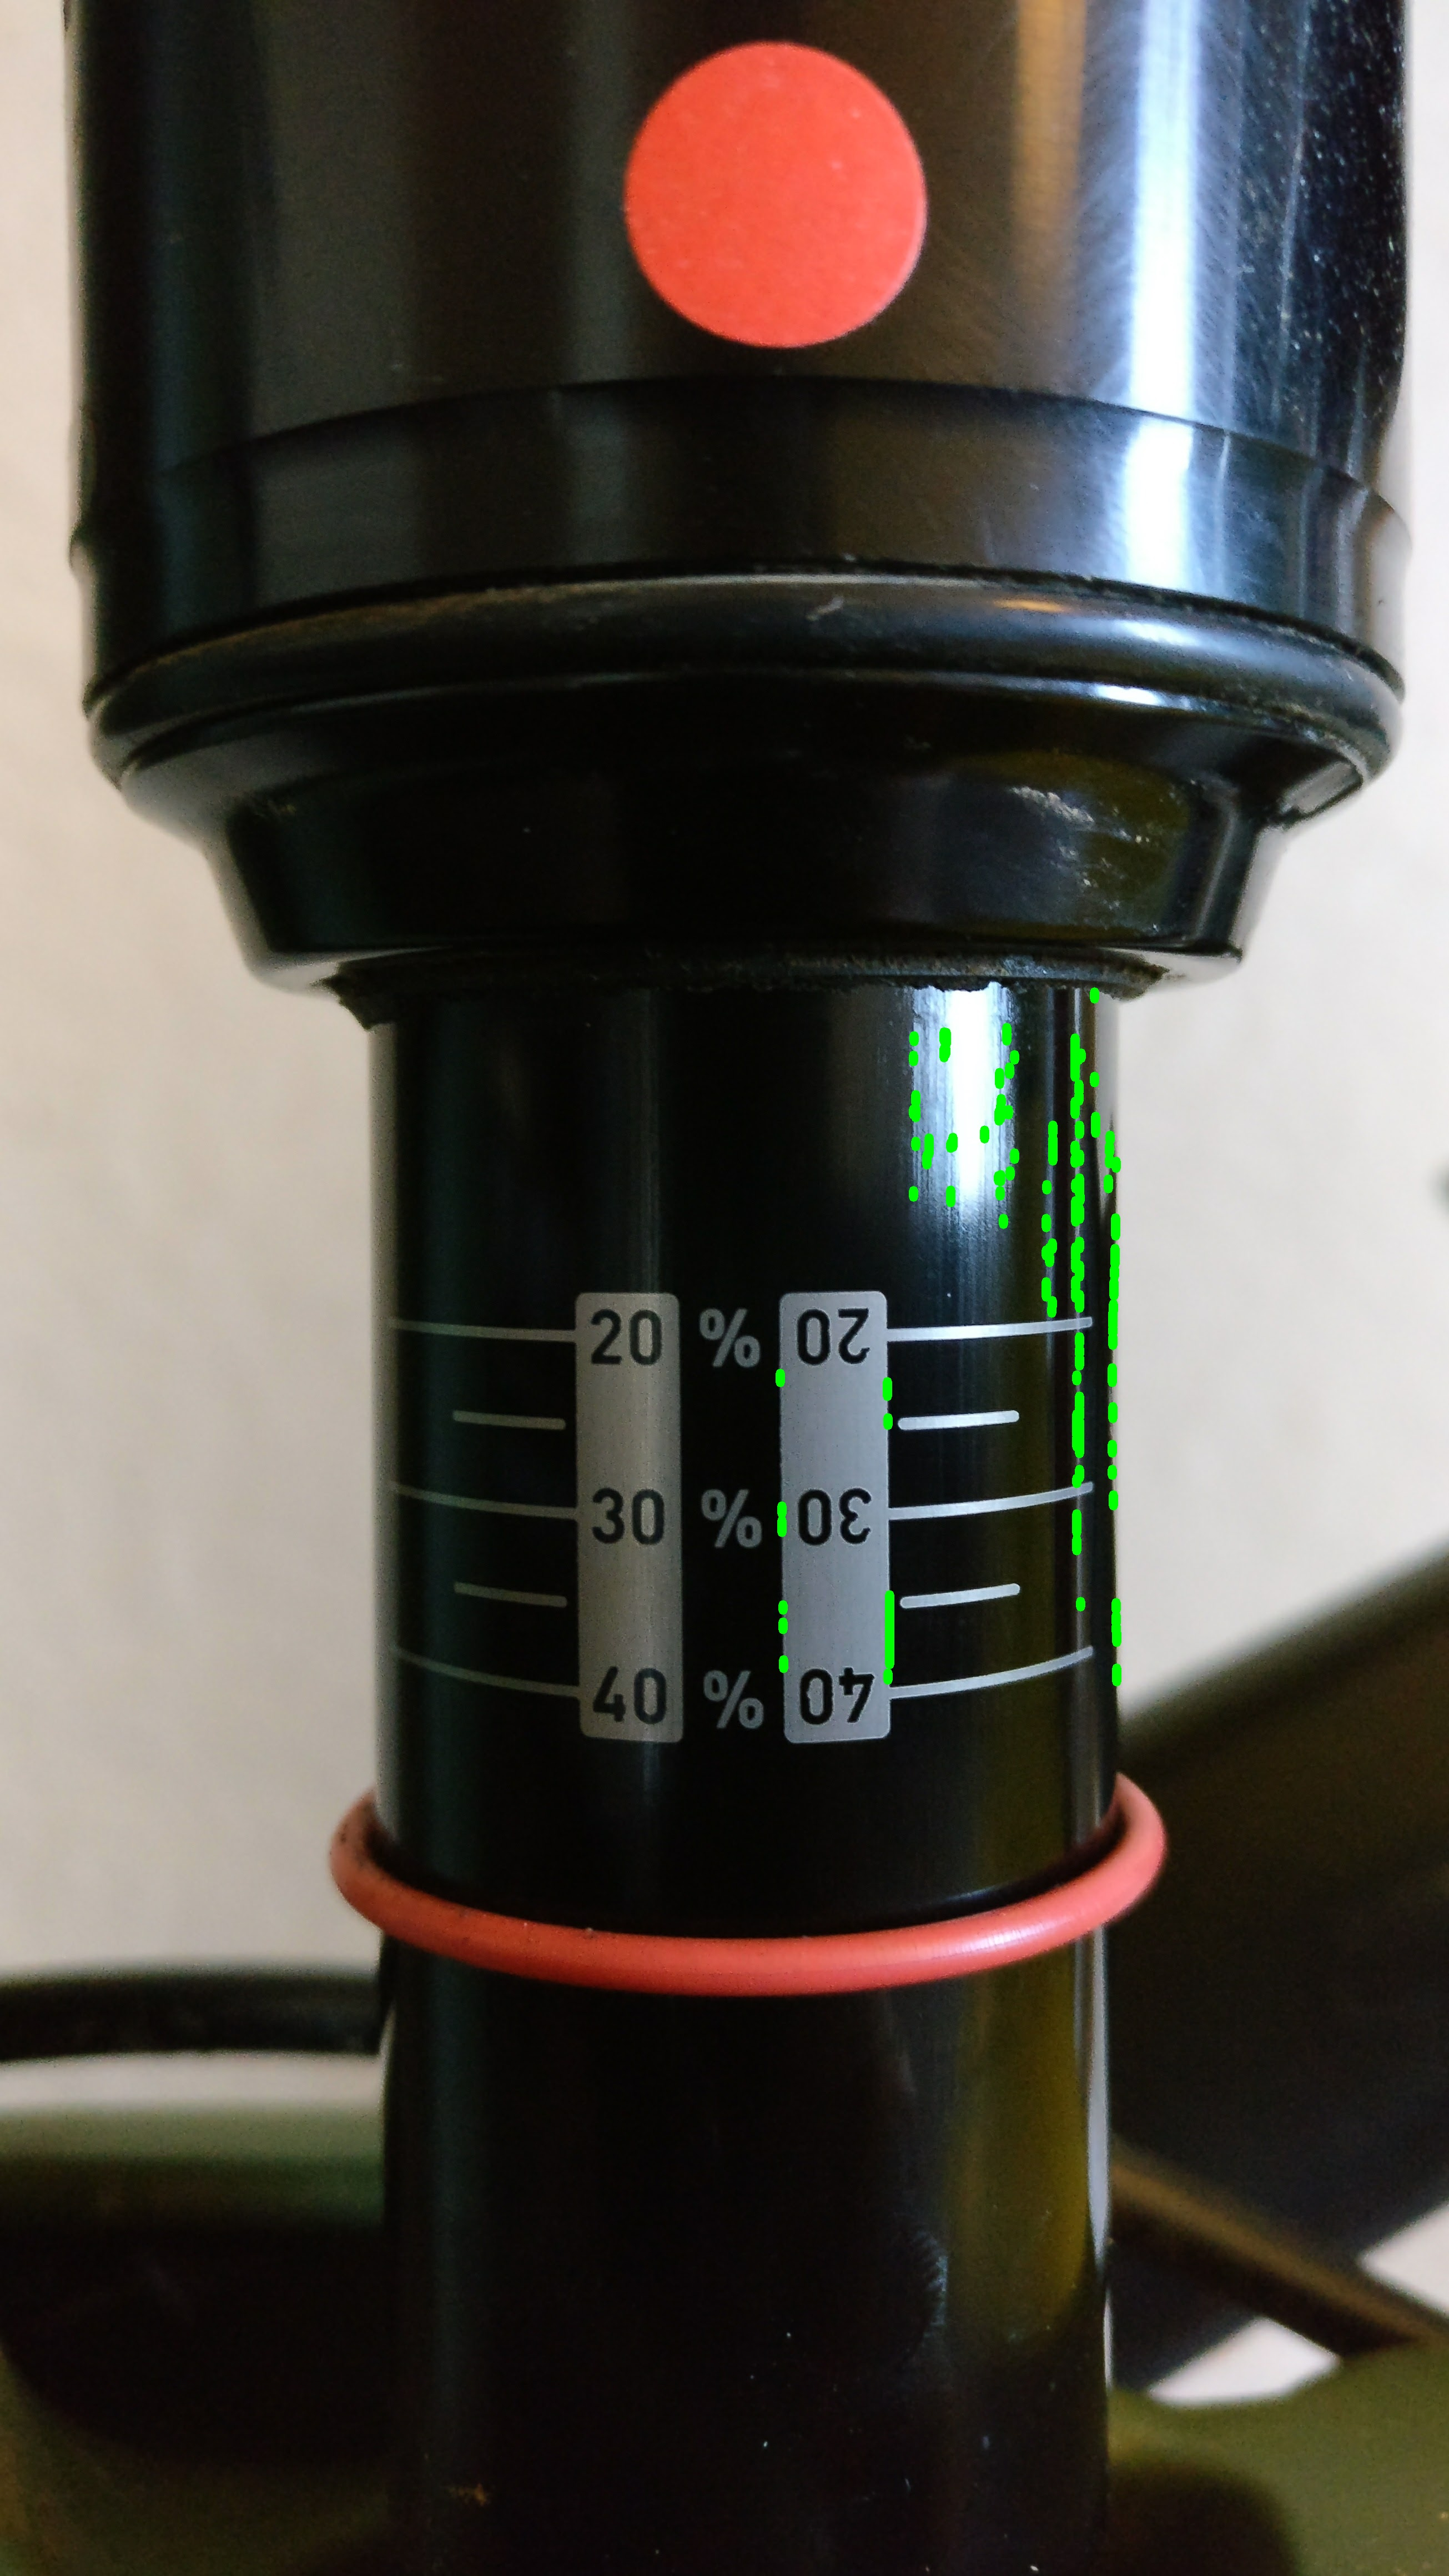
\includegraphics[scale=0.085,
									trim={40cm 35cm 10cm 50cm},
									clip]{../images/results/raw_lines.jpg}
					\caption{Vertical lines in measurement area}
					\label{subfig:lines}
				\end{subfigure}
				\caption{Measurement process using edge detection and Hough lines}
			\end{figure}
		\paragraph{Equation}
			Once the measurements for the shock pressurised to 100 PSI and 150 PSI are produced, they can then be utilised to create a linear equation. This is carried out using Python’s Scipy package and its {\ttfamily linregress} method which accepts two arrays of data and returns the slope and intercept of the linear equation, the code for this can be seen in appendix \ref{app:source_pressure_calculator} lines 32-38. An example equation which is visually described in the chart shown in Figure \ref{fig:equation_plot} is only produced virtually and never output to the user.
			\begin{figure}[h!]
				\centering
				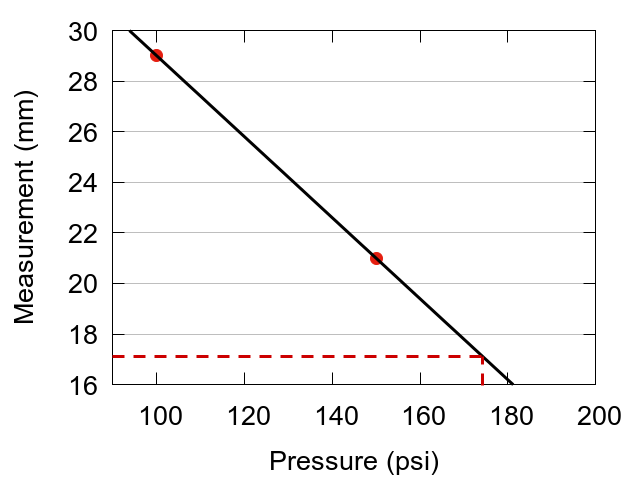
\includegraphics[scale=0.4]{../images/results/scatter_dotted.png}
				\caption{Example of linear equation plot}
				\label{fig:equation_plot}
			\end{figure}
		\paragraph{Produce Setting}
			To produce the final setting the optimal distance that the shock should move to give the desired sag setting is first calculated using data input by the user. For example if the shock stroke is 57mm and the desired sag is 30\% then the desired movement is 17.1mm. This and the equation produced in the previous section are used to calculate the optimal pressure. For example if the equation is $-5:017x+246.426$ then the pressure required to give optimal sag is 161 PSI.
\clearpage
	\subsection{Evaluation}\label{sec:evaluation}
		The following section will describe the results of applying the evaluation techniques outlined in section \ref{sec:methodology_evaluation} to the final prototype application. The outcome of the evaluation gives an indication of how successful the application is at meeting its intended goals and the success of the methods used in the project.
		\subsubsection{Validation}\label{sec:evaluation_validation}
			% Display test results
			% Explain they work and have suitable coverage
			% Explain not full coverage
			Figure \ref{fig:test_results} shows an extract from the testing report produced by the Pycharm \gls{ide}. It includes each unit test for both classes and clearly indicates that the final prototype application successfully passed them all. These included checks to see whether the outputs produced by the application are within an expected range. By doing so this validates not only that the application works but that it also produces results within the anticipated range. The test code can be seen in appendix \ref{app:source}.
			\begin{figure}[h!]
				\centering
				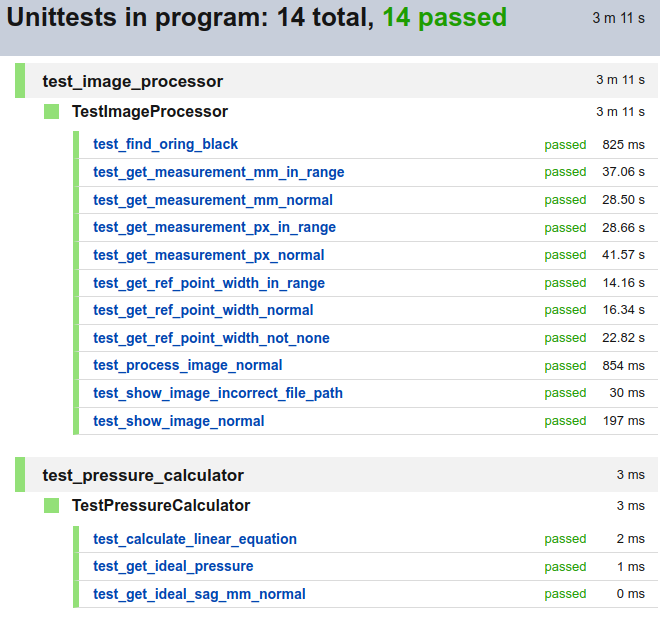
\includegraphics[scale=0.5]{../images/results/test_results.png}
				\caption{Unit test results}
				\label{fig:test_results}
			\end{figure}\\
			Figure \ref{fig:coverage} shows the test coverage report for the application. As stated in section \ref{sec:project_testing_scope} the goal for this project was 100\% test coverage of the application. This has not been achieved but has come close with 97\% of the application being covered. 
			\\\\
			The {\ttfamily main.py} file has no coverage as it is a script as opposed to a testable Class. This is not an issue as it contains the argument parsing and calls to other classes which are not vital to test as the Argparse module is well tested already and the lower level classes have their own testing. The {\ttfamily image\_processor.py} class does not have full coverage as this includes lines which check if outputs provided by OpenCV are valid and close the application if something has gone wrong. The conditions under which these lines are hit could not be recreated due to the irregularity with which problems occur. However testing these lines would not validate the application’s normal functionality.
			\begin{figure}[h!]
				\centering
				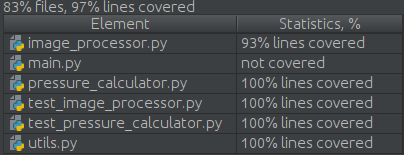
\includegraphics[scale=0.7]{../images/results/coverage.png}
				\caption{Test coverage results}
				\label{fig:coverage}
			\end{figure}
		\subsubsection{Reliability and Accuracy}
		% Describe calculation for two shocks
			% Describe differences between HV and LV
		% Explain why results are good (Working in rounded numbers)
			Table \ref{tab:uncertainty} shows the results of calculating uncertainty for the application under different conditions. The calculations were carried out for two different shocks with two different coloured O-rings, and for two sag settings on each. For the tests the application was run 10 times using the same images and arguments with every output collected, and used in the calculation.
			\rowcolors{2}{white}{white}
			\begin{table}[h!]
				\centering
				\caption{Table of uncertainty calculation results}
				\label{tab:uncertainty}
				\begin{tabular}{|l|r|r|r|r|}
					\hline
					\rowcolor{gray!50}
					&\multicolumn{2}{|l|}{\bfseries High Volume, Red O-Ring}&\multicolumn{2}{|l|}{\bfseries Low Volume, Black O-Ring}\\
					\cline{2-5}&\bfseries 25\%&\bfseries 30\%&\bfseries 25\%&\bfseries 30\%\\
					\hline
					\rowcolor{gray!25}
					\cellcolor{white}&175.02&160.97&133.31&120.54\\
					&174.84&160.52&133.28&120.47\\
					\rowcolor{gray!25}
					\cellcolor{white}&174.95&160.41&133.42&120.48\\
					&174.83&160.65&133.42&120.46\\
					\rowcolor{gray!25}
					\cellcolor{white}{\bfseries Measurements}&174.94&160.75&133.29&120.53\\
					&174.86&160.50&133.38&120.51\\
					\rowcolor{gray!25}
					\cellcolor{white}&175.63&160.48&133.35&120.50\\
					&174.78&160.77&133.36&120.46\\
					\rowcolor{gray!25}
					\cellcolor{white}&175.29&160.57&133.36&120.46\\
					&174.84&160.74&133.42&120.50\\
					\hline
					\rowcolor{gray!25}
					\bfseries Average&175.00&160.64&133.36&120.49\\
					\bfseries Standard Deviation&0.27&0.17&0.05&0.03\\
					\rowcolor{gray!25}
					\bfseries Uncertainty&175 $\pm$ 0.27&160.64 $\pm$ 0.17&133.36 $\pm$ 0.05&120.49 $\pm$ 0.03\\
					\hline
				\end{tabular}
			\end{table}
			\\
			For each test the variances are low, (the highest being $\pm$0.27), which indicates that the application is capable of consistently producing correct sag settings. If these uncertainty measures had been much higher then the settings produced by the application could not have been considered reliable. The calculated setting produced by the application is also rounded to the nearest whole number as increments of less than 1 PSI in a mountain bike shock have negligible effect. Even the most advanced, digital shock pumps do not display fractions of PSI and professional race teams do not make changes of less than 1 PSI. This knowledge further reinforces the capabilities of the application.
			\\\\
			The results for the shock with a red O-ring are slightly higher than those for the black O-ring. This is because the method for finding and applying a boundary to the red O-ring produces a larger variance in results than the method for finding and applying a boundary to the black O-ring. However, the minor difference between the results is insignificant as both colours of O-ring produce accurate results.
		\subsubsection{Comparison to Alternative Methods}\label{sec:alt_methods}
			% Compare results to manual setup
				% Two pressures to put in are known so easy
				% No trial and error, you just do it
			As outlined in section \ref{sec:methodology_manual}, the results generated by the application were compared with the manual, trial and error, method of setting up sag. For this experiment the target sag was 30\% of a 57mm shock stroke equalling a target measurement of 17.1mm. To begin the rider was weighed wearing their normal riding clothing and equipment with the result being approximately 160lbs. Following the manufacturer’s recommended process, the shock was then pressurised to 160 PSI and loaded by the rider. Each of the subsequent steps followed in the trial and error process are shown in Table \ref{tab:manual_process}.
			\rowcolors{2}{gray!25}{white}
			\begin{table}[h!]
				\centering
				\caption{Stages of manual sag setting process}
				\label{tab:manual_process}
				\begin{tabular}{|r|r|l|r|}
					\hline
					\rowcolor{gray!50}
					\bfseries Stage&\bfseries Pressure(PSI)&\bfseries Outcome&\bfseries Action\\
					\hline
					1&160&Too little&+5\\
					2&165&Too little&+20\\
					3&185&Too little&+5\\
					4&190&Too little&+10\\
					5&200&Hit target&N/A\\
					\hline
				\end{tabular}
			\end{table}\\
			To produce the correct sag setting using the manual process required 5 separate adjustments each including pressurisation of the shock, weighting of the bike, and measurement of the marker O-ring. For this particular shock, small changes in pressure made no noticeable difference to the amount of movement so an additional 20 PSI was added in stage 2. Even though there is a chance that the manufacturer’s recommended setting will be correct or very close, the majority of the time a manual set-up needs 4 or more adjustments. Conversely, using the application only involves 3 easy to follow stages and produced reliable results meaning optimal setup can be achieved quicker and with far less effort. The application also removes both the need to weigh the rider and to refer to the manufacturer’s recommended pressure setting which further simplifies the process and saves time. 
			\\\\
			It should be noted that there is disparity between the pressure that results from following the manual process (seen in Table \ref{tab:manual_process}) and that produced by the application (seen in Table \ref{tab:uncertainty}). As the images used during development of the application were of a shock that had not been weighted while the rider was wearing correct clothing and equipment, new images were produced to match the conditions during the manual process and the application retested. This produced a result of 176 PSI which was closer to, but still lower than, the manually produced result. However, when the shock is pressurised to this setting, the sag appears correct. 
			\\\\
			A manual setting was produced for the low volume shock to further investigate this issue. It was found that under these conditions both the manual and application’s results were extremely close at approximately 120 PSI. As high volume shocks require much higher pressures than low volume shocks, it is believed that as the manual pressure of 200 PSI lies above the two pressures which the shock is pressurised to when using the application, this creates inaccurate results. For comparison, the low volume target pressure of 120 PSI lies between the 100 and 150 PSI required by the application. A solution to this will be discussed in section \ref{sec:conclusion_future_work}.
		\subsubsection{Professional Opinion}
			As outlined in section \ref{sec:methodology_professional_opinion}, once the application was complete the Mountain Bike Centre of Scotland were contacted to arrange a meeting with an individual from the industry to demonstrate the application and collect their feedback. The meeting was arranged with Geraint Florida-Jones of the Centre and Mark Ravilious, a mechanical engineer who has ventured into the design and manufacture of his own full suspension frame. Both Mark and Geraint are familiar with the current products that are similar to the application produced by this project such as Shockwiz \citep{quarq2017shockwiz} and the Fox IRD application \citep{foxird}.
			\\\\
			Once Mark and Geraint were familiar with the context of the project and operation of the application, they were asked for their feedback. They both stated that the project had been well executed and the application was simple to operate. Both verified that the setting produced appeared correct for the given shock, bike, and rider’s weight. Furthermore, both agreed that they would recommend the application to the target audience of beginner and intermediate riders though a more professional setup was required for those at the competitive end of the sport.
			\\\\
			Both said that the application produced in this project should be released as a mobile application as this would make it much more user friendly compared to the prototype command line application. Additionally, both stated that more features should be added to provide a more rounded user experience and their suggestions will be explored in section \ref{sec:conclusion_future_work}. Mark questioned the application of a linear equation to a non-linear air shock though once the experiments into linearity, outlined in section \ref{sec:results_pressure_calculation}, were explained he agreed that the shock could be considered linear within the range of its stroke that sag can be adjusted. A written statement from Geraint can be seen in appendix \ref{app:eval_statements}.
			\\\\
			The application was also demonstrated to the staff at Pedals\footnote{\url{http://pedalsbikecare.co.uk/}} bike shop in Edinburgh. Here it received much the same feedback as it got during the meeting with Mark and Geraint; namely that it is a good execution of the concept and with more features would make a mobile application that is entirely suitable for the target demographic. 
			\\\\
			The positive reception that the application received from professionals within the cycling industry demonstrates that it is a suitable prototype which produces correct settings in an easy to use manner. The only issues suggested were the lack of additional features and functionality which is addressed in section \ref{sec:conclusion_future_work}.